% =====================================================================
%  RESEARCH INTERNSHIP REPORT — ISSAT Sousse, 1st Year Engineering Cycle
%  Melki Ayoub
%  PPO-Guided Latent Diffusion for Visual Counterfactual Explanations
%  in Chest Radiography (RSNA dataset)
%
%  Compile:  pdflatex main && pdflatex main && pdflatex main
%  (three passes: ToC/LoF/LoT + hyperref anchors)
% =====================================================================
\documentclass[11pt,a4paper,oneside]{report}

% =====================================================================
%  Preamble — packages, page geometry, heading style
%  Package set kept deliberately close to report/report.tex (the working
%  setup already in the repo) so this compiles on the same TeX Live.
% =====================================================================

\usepackage[a4paper,inner=3.2cm,outer=2.5cm,top=2.8cm,bottom=2.8cm]{geometry}
\usepackage[T1]{fontenc}
\usepackage[utf8]{inputenc}
\usepackage{times}
\usepackage{amsmath,amssymb}
\usepackage{graphicx}
\usepackage{booktabs}
\usepackage{longtable}
\usepackage{array}
\usepackage{caption}
\usepackage{subcaption}
\usepackage{xcolor}
\usepackage{enumitem}
\usepackage{fancyhdr}
\usepackage{url}
\usepackage[hidelinks]{hyperref}
% Allow \path to break at these characters, with NO stretch glue — otherwise
% justification visibly spaces out filenames like "factory / finetuning . py".
\Urlmuskip=0mu
\def\UrlBreaks{\do\/\do\_\do\-\do\.\do\=\do\{\do\}}
% NOTE: titlesec and emptypage are not present in this TeX installation, so
% the chapter heading style below is implemented directly against the report
% class rather than through titlesec.

\hypersetup{
  colorlinks=true,
  linkcolor=black,
  citecolor=blue!45!black,
  urlcolor=blue!45!black,
  pdftitle={PPO-Guided Latent Diffusion for Visual Counterfactual
            Explanations in Chest Radiography},
  pdfauthor={Melki Ayoub}
}

\graphicspath{{figures/}{logos/}}

% ── Headings: "Chapter N" above a large bold title, matching the reference ──
\makeatletter
\renewcommand{\@makechapterhead}[1]{%
  \vspace*{20pt}%
  {\parindent\z@\raggedright\normalfont
   \ifnum\c@secnumdepth>\m@ne
     \huge\bfseries\@chapapp\space\thechapter
     \par\nobreak\vskip 18\p@
   \fi
   \Huge\bfseries #1\par\nobreak
   \vskip 34\p@}}
\renewcommand{\@makeschapterhead}[1]{%
  \vspace*{20pt}%
  {\parindent\z@\raggedright\normalfont
   \Huge\bfseries #1\par\nobreak
   \vskip 34\p@}}
\makeatother

% Roman-numeral top-level sections (I, II, III …) as in the reference report
\renewcommand{\thesection}{\Roman{section}}
\renewcommand{\thesubsection}{\arabic{subsection}}
\renewcommand{\thesubsubsection}{\arabic{subsection}.\arabic{subsubsection}}

% ── Running heads ──────────────────────────────────────────────────────
% Single-sided: every page is "odd", so L/R apply to all pages.
\pagestyle{fancy}
\fancyhf{}
\fancyhead[L]{\small\nouppercase{\leftmark}}
\fancyhead[R]{\small\nouppercase{\rightmark}}
\fancyfoot[C]{\thepage}
\renewcommand{\headrulewidth}{0.4pt}
\fancypagestyle{plain}{%
  \fancyhf{}\fancyfoot[C]{\thepage}\renewcommand{\headrulewidth}{0pt}}

% ── Convenience macros ─────────────────────────────────────────────────
\newcommand{\ntop}{n$\rightarrow$p}
\newcommand{\pton}{p$\rightarrow$n}
% \file{} typesets a path/filename in monospace. Long names such as
% run_eval_ppo.slurm are otherwise unbreakable and overflow the margin, so
% \path (from url) is used to permit line breaks at / . _ and - .
\newcommand{\file}[1]{\texttt{\path{#1}}}
\newcommand{\Rterm}[1]{$R_{\text{#1}}$}

% Logo helper: draw the logo if the file was supplied, otherwise fall back
% to a text placeholder so the document always compiles.
\newcommand{\logoorname}[3]{%
  \IfFileExists{#1}{\includegraphics[height=#2]{#1}}{\parbox{0.35\textwidth}{\centering\small\textsc{#3}}}%
}

\captionsetup{font=small,labelfont=bf}
\setlength{\parskip}{0.35em}


\begin{document}

% ── Front matter ────────────────────────────────────────────────────
% (report class has no \frontmatter; roman numbering is set directly)
% Front matter uses \pagestyle{plain}: page number only, no running heads —
% otherwise \leftmark and \rightmark are both "Contents" and duplicate.
\pagenumbering{roman}
\pagestyle{plain}

% =====================================================================
%  Cover page
%  LOGOS: logos/ISSATSo_logo.jpg and logos/SDU.png. Each is wrapped in
%  \IfFileExists so the page still builds (with a text fallback) if a
%  logo file is ever missing.
% =====================================================================
\thispagestyle{empty}

\begin{center}

{\large\scshape Tunisian Republic}\\[2pt]
{\normalsize\scshape Ministry of Higher Education and Scientific Research}\\[10pt]
{\normalsize\scshape University of Sousse}\\[2pt]
{\normalsize\scshape Higher Institute of Applied Sciences and Technology of Sousse}\\[10pt]

% ISSAT logo. The source JPEG (2624x1828) carries a wide white margin, so it
% is trimmed (left bottom right top, in bp) and clipped before scaling —
% otherwise the visible mark is only ~60% of the reserved height.
\IfFileExists{logos/ISSATSo_logo.jpg}
  {
\includegraphics[trim=55 300 90 320,clip,height=2.75cm]{logos/ISSATSo_logo.jpg}}
  {\parbox{0.35\textwidth}{\centering\small\textsc{ISSAT Sousse}}}

\vspace{10pt}
\rule{\textwidth}{1.2pt}

\vspace{10pt}
{\Huge\scshape Research Internship Report}
\vspace{8pt}

\rule{\textwidth}{1.2pt}

\vspace{14pt}
{\large\scshape Class: 1st Year Engineering Cycle}

\vspace{12pt}
{\itshape Presented by:}\\[6pt]
{\Large\scshape Melki Ayoub}

\vspace{14pt}
\rule{0.85\textwidth}{0.6pt}\\[8pt]
{\large\itshape PPO-Guided Latent Diffusion for Visual Counterfactual\\
Explanations in Chest Radiography (RSNA Dataset)}\\[8pt]
\rule{0.85\textwidth}{0.6pt}

\vspace{14pt}
{\large\scshape Host Institution:}\\[6pt]

% SDU logo already contains the wordmark "University of Southern Denmark",
% so the line below it is dropped when the logo is present to avoid
% printing the institution name twice.
\IfFileExists{logos/SDU.png}
  {
\includegraphics[height=1.9cm]{logos/SDU.png}\\[8pt]}
  {{\large University of Southern Denmark (SDU)}\\[2pt]}

{\normalsize Maersk Mc-Kinney Moller Institute}\\[2pt]
{\itshape Remote Research Internship}

\vspace{12pt}
{\itshape Academic Supervisor:}\\[5pt]
{\large Professor Sadok Ben Yahia}

\vspace{10pt}
{\itshape Internship Period:}\\[5pt]
15/06/2026 \quad--\quad 15/08/2026

\vspace{8pt}
{Academic Year: 2025--2026}

\end{center}

\clearpage

\chapter*{Acknowledgments}
\addcontentsline{toc}{chapter}{Acknowledgments}
\markboth{Acknowledgments}{}

I would like to express my sincere gratitude to the Maersk Mc-Kinney
Moller Institute at the University of Southern Denmark for hosting this
research internship and for granting me the freedom to pursue an open
research question rather than a predefined implementation task.

I especially thank my academic supervisor, \textbf{Professor Sadok Ben
Yahia}, for his guidance, his availability throughout the internship, and
for the methodological rigour he insisted upon --- in particular the
demand that every claimed result be verified against an independent
control rather than accepted at face value. That principle shaped the
most valuable finding of this work.

I also thank the ISSAT Sousse teaching staff for the academic preparation
that made this project possible, and the administrators of the
high-performance computing cluster on which every experiment reported
here was executed.

\clearpage


\tableofcontents
\clearpage
\listoffigures
\clearpage
\listoftables
\clearpage

\chapter*{Acronyms}
\addcontentsline{toc}{chapter}{Acronyms}
\markboth{Acronyms}{}

\begin{itemize}[leftmargin=1.4em,itemsep=2pt]
  \item \textbf{AI}: Artificial Intelligence
  \item \textbf{AUC}: Area Under the (ROC) Curve
  \item \textbf{BCE}: Binary Cross-Entropy
  \item \textbf{BDC}: Breast Density Contrast
  \item \textbf{CAM}: Class Activation Map
  \item \textbf{CBIS-DDSM}: Curated Breast Imaging Subset of the Digital
        Database for Screening Mammography
  \item \textbf{CTR}: Cardio-Thoracic Ratio
  \item \textbf{CV}: Counterfactual Validity
  \item \textbf{CXR}: Chest X-Ray (chest radiograph)
  \item \textbf{DDIM}: Denoising Diffusion Implicit Model
  \item \textbf{DICOM}: Digital Imaging and Communications in Medicine
  \item \textbf{FID}: Fr\'echet Inception Distance
  \item \textbf{FOP}: Foreign-Object Preservation
  \item \textbf{GAE}: Generalized Advantage Estimation
  \item \textbf{GPU}: Graphics Processing Unit
  \item \textbf{Grad-CAM}: Gradient-weighted Class Activation Mapping
  \item \textbf{HF-corr}: High-Frequency Correlation
  \item \textbf{HPC}: High-Performance Computing
  \item \textbf{IP}: Identity Preservation
  \item \textbf{ISSAT}: Higher Institute of Applied Sciences and Technology of Sousse
  \item \textbf{JSON}: JavaScript Object Notation
  \item \textbf{L1 / L2}: Absolute-value / squared-error norms
  \item \textbf{LHR}: Lesion Hit Rate
  \item \textbf{LLR}: Lesion Load Ratio
  \item \textbf{LoRA}: Low-Rank Adaptation
  \item \textbf{MAE}: Mean Absolute Error
  \item \textbf{MDP}: Markov Decision Process
  \item \textbf{MLP}: Multi-Layer Perceptron
  \item \textbf{MOP}: Marker/clip Preservation
  \item \textbf{MS-SSIM}: Multi-Scale Structural Similarity Index Measure
  \item \textbf{MSI}: Margin Spiculation Index
  \item \textbf{PEFT}: Parameter-Efficient Fine-Tuning
  \item \textbf{PPO}: Proximal Policy Optimization
  \item \textbf{PSPNet}: Pyramid Scene Parsing Network
  \item \textbf{RL}: Reinforcement Learning
  \item \textbf{RSNA}: Radiological Society of North America
  \item \textbf{SCP}: Costophrenic-recess Score (\textit{score costo-phr\'enique})
  \item \textbf{SD1.5}: Stable Diffusion version 1.5
  \item \textbf{SDU}: University of Southern Denmark
  \item \textbf{SLURM}: Simple Linux Utility for Resource Management
  \item \textbf{VAE}: Variational Autoencoder
  \item \textbf{VRAM}: Video Random-Access Memory
  \item \textbf{XAI}: Explainable Artificial Intelligence
  \item \textbf{XRV}: TorchXRayVision
  \item \textbf{YOLO}: You Only Look Once (object-detection family)
\end{itemize}

\clearpage


% ── Main matter ─────────────────────────────────────────────────────
\clearpage
\pagenumbering{arabic}
\setcounter{page}{1}
\pagestyle{fancy}

\chapter*{General Introduction}
\addcontentsline{toc}{chapter}{General Introduction}
\markboth{General Introduction}{}

The transition from theoretical academic study to the practice of
scientific research is a decisive stage in an engineer's training. This
report documents the work carried out during a research internship
completed as part of the first year of the engineering cycle at the
Higher Institute of Applied Sciences and Technology of Sousse (ISSAT
Sousse), hosted remotely by the Maersk Mc-Kinney Moller Institute at the
University of Southern Denmark (SDU).

Deep neural classifiers now reach expert-level accuracy on many medical
imaging tasks, but their clinical adoption remains constrained by a
question they cannot themselves answer: \emph{why} was this prediction
made? The dominant family of post-hoc explanation methods --- saliency
maps and Grad-CAM among them --- answers only \emph{where} the model is
looking. It does not say \emph{what} would have to change for the
decision to be different. For a radiologist auditing a pneumonia
classifier, a heatmap over the right lower lobe is a far weaker statement
than an image showing precisely which change to that lobe would flip the
model's verdict.

\textbf{Visual counterfactual explanations} address this gap directly.
Given a query image $x$ and a target class $c$, a counterfactual
generator produces an image $x_c$ such that a classifier $f$ predicts
$f(x_c) \approx c$, while $x_c$ remains a realistic radiograph that
preserves the patient's anatomy and any non-pathological content --- ribs,
mediastinal silhouette, tubes, pacemakers and monitoring leads. The
change between $x$ and $x_c$ \emph{is} the explanation.

This internship investigated a specific research hypothesis in that
setting: that the per-step control of a guided diffusion sampler should
be \emph{learned} rather than fixed. A hand-tuned guidance schedule
applies the same editing effort to every image, which under-edits
difficult cases and over-edits --- and thereby de-realizes --- easy ones.
The system built during this internship instead frames the choice of
per-step sampling parameters as a sequential decision problem and trains
a Proximal Policy Optimization (PPO) agent to solve it, on top of a
Stable Diffusion~1.5 latent generator adapted to chest radiography with
Low-Rank Adaptation (LoRA).

The work was organised around four research questions:

\begin{itemize}[leftmargin=*]
  \item Can a reinforcement-learning agent that controls only the
        \emph{sampling procedure} --- never the diffusion weights ---
        produce valid counterfactuals on chest radiographs?
  \item Can the edits be spatially confined to clinically plausible
        regions, rather than diffusing over the whole image?
  \item Do the resulting counterfactuals encode \emph{genuine disease
        signal}, or do they merely constitute adversarial perturbations
        against the particular classifier used for guidance?
  \item How do the standard counterfactual evaluation metrics of
        Singla~\emph{et al.}~\cite{singla2022} behave under the compute
        constraints of a two-month single-GPU project?
\end{itemize}

The third question turned out to be the scientifically decisive one, and
its answer reshaped the second half of the internship. An independent
held-out validation --- re-scoring the generated counterfactuals with
classifiers that had never participated in the guidance loop --- showed
that a system reporting near-perfect validity against its own guidance
classifier transferred very poorly to independent models. That negative
result, and the redesign it motivated, form the substantive contribution
of this work and are reported in full in Chapter~\ref{ch:results}.

The report is organised into five chapters:

\begin{itemize}[leftmargin=*]
  \item \textbf{Chapter~\ref{ch:context}} presents the internship
        context, the host research institution, and the objectives, work
        packages and expected outcomes of the project.
  \item \textbf{Chapter~\ref{ch:environment}} describes the research and
        development environment: the HPC cluster and its SLURM scheduler,
        the deep-learning frameworks, the pretrained model zoo, and the
        dataset-access tooling.
  \item \textbf{Chapter~\ref{ch:tasks}} details the tasks performed ---
        the architecture of the pipeline, its module-by-module
        construction, and the iterative debugging and redesign cycles
        that the experimental evidence forced.
  \item \textbf{Chapter~\ref{ch:results}} reports the measured results,
        discusses the strengths and the substantial limitations of the
        current system, and sets out realistic perspectives for future
        work.
  \item \textbf{Chapter~\ref{ch:breast}} documents additional,
        self-initiated work extending the pipeline to a second imaging
        domain --- mammography, on the CBIS-DDSM dataset --- undertaken to
        test whether the method and its evaluation discipline generalise
        beyond chest radiography.
\end{itemize}

The RSNA pneumonia system of Chapters~\ref{ch:context}--\ref{ch:results}
remains the core deliverable and the primary subject of this report;
Chapter~\ref{ch:breast} is reported separately, and more briefly, as
additional work rather than as a second fully-validated result standing
alongside the main one.

\clearpage

\chapter{Internship Context Presentation}
\label{ch:context}

This chapter establishes the context of the internship, introduces the
host research institution, and sets out the objectives, work packages and
expected outcomes of the project.

\section{Presentation of the Host Institution}

\subsection{Overview}

The internship was carried out at the \textbf{Maersk Mc-Kinney Moller
Institute}, a research institute of the \textbf{University of Southern
Denmark (SDU)}. The Institute is an academic research environment
organised around robotics, artificial intelligence, embedded systems and
applied data science, and its work is structured around research
questions and publications rather than around product delivery for
clients.

This distinction shaped the entire internship. There was no client, no
specification document and no delivery deadline for a feature set. The
deliverable was a defensible answer to a research question, together
with the experimental apparatus needed to reproduce it --- which, as
Chapter~\ref{ch:results} discusses, includes the apparatus needed to
\emph{disprove} an initially promising result.

\subsection{Internship Framework}

This work fulfils the research internship requirement of the first-year
engineering cycle at ISSAT Sousse. The internship was conducted
\textbf{remotely}, under the academic supervision of \textbf{Professor
Sadok Ben Yahia}, over the period 15 June 2026 to 15 August 2026.

The remote format had a concrete methodological consequence. All
computation ran as batch jobs on a high-performance computing cluster
under the SLURM scheduler, with no interactive session and no ability to
attach a debugger to a running job. Every experiment therefore had to be
specified completely in advance, instrumented well enough to be
diagnosed from its log file alone, and cheap enough to fail fast. This
constraint is visible throughout the engineering choices described in
Chapter~\ref{ch:tasks}.

\section{Context and Objectives of the Internship}

\subsection{Purpose}

Explainable Artificial Intelligence (XAI) for medical imaging is
dominated by attribution methods, which localise evidence but do not
describe the change that would alter a decision. Counterfactual image
generation supplies that missing description, but it introduces a
verification problem of its own: an image that flips a classifier's
output has not necessarily acquired --- or lost --- any disease. It may
simply have acquired an adversarial perturbation tailored to that one
model.

The purpose of this project was therefore twofold:

\begin{itemize}[leftmargin=*]
  \item To build a counterfactual generation system for binary pneumonia
        classification on chest radiographs, in which the diffusion
        sampling schedule is \emph{learned} by a reinforcement-learning
        agent rather than fixed by hand.
  \item To evaluate that system honestly --- including with controls
        capable of exposing the adversarial failure mode --- rather than
        reporting only the metric that the system was optimised against.
\end{itemize}

\subsection{Main Objective}

The central objective was to engineer and evaluate a complete research
pipeline that, given a chest radiograph $x$ and a target class $c$,
produces a counterfactual $x_c$ satisfying three simultaneous criteria:

\begin{enumerate}[leftmargin=*]
  \item \textbf{Validity}: a frozen classifier $f$ scores $x_c$ at the
        target class with a large margin.
  \item \textbf{Realism}: $x_c$ is distributionally indistinguishable
        from genuine radiographs.
  \item \textbf{Identity preservation}: $x_c$ differs from $x$ only in a
        minimal, class-relevant region, leaving patient anatomy and
        foreign objects intact.
\end{enumerate}

The methodological commitment underlying the whole system is that the
diffusion model's \emph{weights} are never optimised by reinforcement
learning. The PPO agent controls only the sampling procedure --- noise
strength, guidance scales, number of refinement passes, and the stopping
decision --- around a frozen, LoRA-adapted generator. This keeps the
action space small and interpretable, and makes the learned policy
reusable across arbitrary query images at inference time.

\subsection{Assigned Work Packages}

The project was decomposed into six work packages:

\begin{itemize}[leftmargin=*]
  \item \textbf{WP1 --- Data ingestion.} Programmatic acquisition of the
        RSNA Pneumonia Detection Challenge dataset, DICOM decoding,
        normalisation, and derivation of a binary label from the
        bounding-box annotations.
  \item \textbf{WP2 --- Pretrained model integration.} Loading and
        freezing a pneumonia classifier, a lung/heart segmentation
        network, and an object-detector feature extractor, all serving as
        fixed sources of guidance and reward signal.
  \item \textbf{WP3 --- Generator adaptation.} Parameter-efficient
        LoRA fine-tuning of a Stable Diffusion~1.5 UNet from the
        natural-image domain to chest radiography.
  \item \textbf{WP4 --- Reinforcement-learning control.} Design of a
        Gym-style environment, a shaped reward function, and a PPO
        actor-critic agent; training of two directional policies, one per
        class-flip direction.
  \item \textbf{WP5 --- Evaluation.} Implementation of the
        Singla~\emph{et al.}~\cite{singla2022} metric suite (CV, FID,
        FOP) plus clinical proxy metrics, and of pixel-level difference
        visualisation.
  \item \textbf{WP6 --- Validation and diagnostics.} Independent
        held-out re-scoring to distinguish genuine disease signal from
        adversarial perturbation, and Grad-CAM analysis of the guidance
        classifier for shortcut learning.
\end{itemize}

WP6 was not part of the initial plan. It was added mid-internship, in
direct response to the observation that the primary validity metric was
computed with the same classifier that had produced the guidance
gradient, and was therefore circular. Its results are the central finding
of this report.

A further piece of work, undertaken after WP1--WP6 and reported separately
in Chapter~\ref{ch:breast}, was not assigned and is not counted among these
six packages: a self-initiated extension of the pipeline to a second
imaging domain, breast-cancer screening mammography, to test whether the
architecture and the WP6 evaluation discipline generalise beyond chest
radiography.

\section{Expected Results}

The anticipated deliverables at the outset of the internship were:

\begin{itemize}[leftmargin=*]
  \item A reproducible, end-to-end research pipeline covering ingestion,
        generator adaptation, policy training and evaluation, executable
        as batch jobs on an HPC cluster.
  \item Two trained directional policies together with their
        checkpoints and configuration provenance.
  \item A quantitative evaluation under the reference metric protocol,
        with the numbers traceable to serialised artefacts rather than
        to transcription.
  \item A critical assessment of what the system does and does not
        demonstrate, including its failure modes.
\end{itemize}

\section{Conclusion}

This chapter has set out the academic research context of the
internship, introduced the Maersk Mc-Kinney Moller Institute as host
institution, and defined the objectives and work packages of the
project. The following chapter details the research and development
environment --- the cluster, the frameworks, and the pretrained model
zoo --- within which this work was carried out.

\chapter{Research and Development Environment}
\label{ch:environment}

This chapter presents the computational infrastructure, software
frameworks, pretrained models and data-access tooling used to design,
train and evaluate the system. Only components actually used in the
project are described, at the exact dependency versions pinned for the
project's environment.

\section{Computing Infrastructure}

\subsection{HPC Cluster and the SLURM Scheduler}

All training and evaluation ran on a shared high-performance computing
cluster managed by \textbf{SLURM} (Simple Linux Utility for Resource
Management)~\cite{yoo2003slurm}, an open-source batch scheduler that
allocates compute nodes to queued jobs according to resource requests and
fair-share priority.

Every stage of the pipeline --- training, evaluation, held-out validation,
classifier probing, and small-scale smoke testing --- runs as its own
batch job, each requesting one GPU, 8 CPU cores and 64\,GB of system
memory on the cluster's GPU partition, and differing mainly in its
walltime request --- a parameter that, as Section~\ref{sec:walltime} of
Chapter~\ref{ch:tasks} describes, turned out to matter a great deal.

Two properties of this environment drove most of the engineering
decisions in Chapter~\ref{ch:tasks}:

\begin{itemize}[leftmargin=*]
  \item \textbf{Compute nodes have no internet access.} Any model weight
        or dataset must be downloaded in advance on the login node, and
        every job is configured to fail immediately, rather than hang
        silently, if it ever attempts a network call it should not need.
  \item \textbf{Jobs are non-interactive and are killed at walltime.} A
        job that exceeds its requested time limit is terminated
        unconditionally, whatever it was doing.
\end{itemize}

\subsection{GPU Hardware}

The cluster is heterogeneous, and the GPU model assigned to a job depends
on which node the scheduler allocates. Two devices were observed across
this project's runs, with measured throughput recorded in the job logs:

\begin{table}[h]
\centering
\caption[GPU hardware and measured runtimes]{GPU hardware observed across
project runs, with measured wall-clock cost of the two main pipeline
halves.}
\label{tab:hardware}
\begin{tabular}{@{}lrrr@{}}
\toprule
\textbf{Device} & \textbf{VRAM} & \textbf{PPO training} & \textbf{Evaluation} \\
\midrule
Tesla P100-PCIE   & 16\,GB & $\sim$20\,h   & $>$4\,h (unfinished) \\
Quadro RTX 5000   & 16\,GB & $\sim$12.5\,h & $\sim$2.5\,h \\
\bottomrule
\end{tabular}
\end{table}

The generator's own memory footprint is modest --- the VAE and UNet
combined occupy an estimated $1826$\,MB --- so the 16\,GB devices
available were never the binding constraint. Wall-clock time was.

\subsection{Environment Provisioning}

A single provisioning step, run once on the login node, creates the
Python virtual environment, installs the pinned dependency set, and ---
most importantly --- \emph{prefetches} every pretrained weight the
compute nodes will later need, including the several TorchXRayVision
DenseNet checkpoints. Dependencies are pinned to exact versions
(\texttt{torch==2.5.1+cu121}, \texttt{diffusers==0.38.0},
\texttt{peft==0.19.1}, \texttt{torchxrayvision==1.5.2},
\texttt{ultralytics==8.4.83}) so that a run months later reproduces the
same numerical environment.

\section{Deep Learning Frameworks}

\subsection{PyTorch}

PyTorch~2.5.1 with CUDA~12.1 is the numerical foundation of the entire
project. Its define-by-run autograd is not merely a convenience here but
a structural requirement: the counterfactual guidance mechanism
differentiates the frozen classifier's loss \emph{with respect to an
intermediate latent inside the diffusion sampling loop}, a gradient path
that must be constructed dynamically at each denoising step. Models run
in half precision on GPU, with selected parameters upcast to full
precision where numerical stability requires it.

\subsection{Diffusers and Stable Diffusion 1.5}

The generator is built on \textbf{Stable Diffusion~1.5}, a latent
diffusion model~\cite{rombach2022} loaded through the Hugging Face
\texttt{diffusers} library. Rather than training a diffusion model from
scratch on a comparatively small medical dataset, the project reuses
SD1.5's pretrained VAE and UNet and adapts only a small parameter subset.

Images of $256\times256$ pixels are encoded by the frozen VAE into a
$4\times32\times32$ latent tensor, an $8\times$ spatial compression that
reduces the cost of every subsequent sampling and guidance step by two
orders of magnitude relative to pixel-space diffusion. Sampling uses
\textbf{DDIM}~\cite{song2021ddim}, whose deterministic, non-Markovian
reverse process permits a partial forward-then-reverse trajectory --- the
mechanism by which an existing radiograph is edited rather than a new
image synthesised from noise.

\subsection{PEFT and LoRA}

Full fine-tuning of the SD1.5 UNet (866~million parameters) was out of
scope for the available compute. \textbf{LoRA}~\cite{hu2021lora}, applied
through the Hugging Face \texttt{peft} library, instead freezes the
pretrained weights and injects trainable low-rank matrix pairs into
selected projections --- here the attention layers' query, key, value and
output projections, at rank 16 with $\alpha=16$ and dropout $0.05$.

The resulting parameter economy is exact: \textbf{6{,}782{,}976 trainable
parameters out of 866{,}303{,}940}, or \textbf{0.78\%} of the model. This
is what made domain adaptation feasible within the internship's compute
budget.

\section{Pretrained Model Zoo}

The system depends on three frozen pretrained networks, none of which is
ever updated by training. They supply, respectively, the guidance
gradient, the spatial constraint, and part of the preservation signal.

\subsection{TorchXRayVision}

\textbf{TorchXRayVision} (XRV)~\cite{cohen2022xrv} is a library of chest
X-ray datasets and pretrained models with a standardised preprocessing
convention. It supplies two distinct components here:

\begin{itemize}[leftmargin=*]
  \item \textbf{Classifiers} --- DenseNet-121 models trained independently
        on different chest X-ray corpora (RSNA, CheXpert, NIH, MIMIC-CXR,
        PadChest) and exposed under a common interface. The availability
        of \emph{multiple independently trained} classifiers over a
        shared label space is what makes the held-out validation of
        Chapter~\ref{ch:results} possible at all; this is the single
        most consequential tooling choice in the project.
  \item \textbf{Segmentation} --- a \textbf{PSPNet} providing per-anatomy
        masks. The lung channels gate where editing is permitted; the
        heart and lung channels together yield the Cardio-Thoracic Ratio
        used as a clinical proxy metric.
\end{itemize}

\subsection{YOLOv8}

\textbf{YOLOv8}~\cite{jocher2023yolov8} (nano variant, loaded via
\texttt{ultralytics}) is used not as a detector but as a \emph{frozen
feature extractor}. Its backbone embedding of an image serves as a
coarse proxy for structural and foreign-object content: penalising drift
in this embedding discourages the generator from destroying tubes, leads
and other hardware. It also underlies the costophrenic-recess proxy
metric.

The report is explicit that this is an approximation. YOLOv8n is
pretrained on COCO, a natural-image corpus, and is not a
radiograph-specific device detector; Section~\ref{sec:limitations}
discusses the consequences.

\subsection{Grad-CAM}

\textbf{Grad-CAM}~\cite{selvaraju2017gradcam} produces class-discriminative
localisation maps by weighting convolutional feature maps with the
gradients flowing into them. A single shared implementation serves two
distinct roles in this project:

\begin{itemize}[leftmargin=*]
  \item \textbf{Diagnostic} --- rendering Grad-CAM overlays to check
        whether the guidance classifier attends to lung pathology or to
        a global brightness/contrast shortcut.
  \item \textbf{Constraint} --- the same map, thresholded and feathered,
        restricts the region in which the PPO agent is permitted to edit
        (Chapter~\ref{ch:tasks}, Section~\ref{sec:gradcam_mask}).
\end{itemize}

\section{Data Access}

The \textbf{RSNA Pneumonia Detection Challenge} dataset~\cite{rsna2018}
is retrieved programmatically through \texttt{kagglehub}, which handles
authentication and local caching so that a compute node can later read
the data with no network access. Images arrive as DICOM and are decoded
with \texttt{pydicom} (with \texttt{pylibjpeg} for JPEG-compressed
transfer syntaxes), min--max normalised to $[0,1]$ and resized to
$256\times256$.

The corpus actually loaded comprises \textbf{26{,}684 studies}, of which
\textbf{6{,}012 are pneumonia-positive} and \textbf{20{,}672 negative} ---
a $22.5\%$ positive rate whose consequences for training are discussed
in Chapter~\ref{ch:tasks}.

\section{Toolchain Summary}

\begin{table}[h]
\centering
\caption{Research and development environment summary.}
\label{tab:toolchain}
\begin{tabular}{@{}p{0.28\textwidth}p{0.62\textwidth}@{}}
\toprule
\textbf{Category} & \textbf{Tools / Technologies} \\
\midrule
Compute infrastructure & SLURM batch scheduler; Tesla P100-PCIE-16GB and
Quadro RTX 5000 GPU nodes; offline (no-internet) compute nodes \\
Numerical framework & PyTorch 2.5.1 + CUDA 12.1, half-precision inference \\
Generative model & Stable Diffusion 1.5 via \texttt{diffusers} 0.38.0; DDIM sampling \\
Parameter-efficient tuning & LoRA via \texttt{peft} 0.19.1 (rank 16, $\alpha$ 16) \\
Pretrained medical models & TorchXRayVision 1.5.2 (DenseNet-121 classifiers, PSPNet segmenter) \\
Object-detection features & Ultralytics YOLOv8n 8.4.83 \\
Explainability & Grad-CAM (custom shared implementation) \\
Data access & \texttt{kagglehub}, \texttt{pydicom}, \texttt{pylibjpeg} \\
Scientific stack & NumPy, SciPy, scikit-image, scikit-learn, Matplotlib \\
Version control & Git \\
\bottomrule
\end{tabular}
\end{table}

\section{Conclusion}

This chapter has described the computational environment of the
internship: a non-interactive, offline, walltime-bounded HPC cluster, a
PyTorch-based generative stack, and a set of frozen pretrained medical
models. The next chapter details how these components were assembled into
a working research pipeline, and how experimental evidence repeatedly
forced that pipeline to be redesigned.

\chapter{Presentation of the Tasks Performed}
\label{ch:tasks}

This chapter details the technical work carried out during the
internship: the architecture of the research pipeline, the construction
of each of its modules, and --- occupying the larger part of the
internship --- the successive redesign cycles that experimental evidence
forced upon it.

\section{Global Pipeline Architecture}

\subsection{Delivered Functional Flow}

The system is organised as a single linear data flow, split across two
independent executable entry points that share a common construction
layer:

\begin{enumerate}[leftmargin=*]
  \item \file{ingestion.py} downloads the RSNA dataset and exposes it as
        an \texttt{RSNACXRDataset}.
  \item \file{pipeline.py}'s \texttt{build\_common()} constructs the
        dataset, the frozen models and the generator. Both entry points
        call it, which guarantees that training and evaluation operate on
        \emph{identical} objects.
  \item \file{src/models.py} loads and freezes the classifier, the
        PSPNet segmenter and the YOLOv8 feature extractor.
  \item \file{src/generator.py} and \file{factory/finetuning.py}
        adapt the Stable Diffusion UNet to the radiograph domain via
        LoRA.
  \item \file{factory/environment.py} and \file{factory/ppo.py} train
        two directional PPO policies.
  \item \file{eval_main.py} reloads the checkpoints and runs
        \file{src/metrics.py} and \file{src/diff_viz.py}.
\end{enumerate}

Alongside this main path sit two diagnostic tools that never participate
in training: \file{heldout_validation.py} and
\file{check_classifier_localization.py}.

\subsection{Splitting Training from Evaluation}
\label{sec:walltime}

The pipeline was originally a single process, \file{main.py}, that
trained both policies and then evaluated them. This design failed
concretely. Job \textbf{17644171} completed PPO training, wrote both
policies to disk, and was then killed at the 24-hour walltime boundary
partway through evaluation. No metrics were produced, and --- critically
--- no entry point existed that could reload the surviving policies. A
full training run had to be repeated to recover a number that the
finished policies could already have produced.

The pipeline was restructured in response. \file{main.py} now performs
Steps~1--5 (training) and terminates after writing checkpoints;
\file{eval_main.py} performs Steps~6--6B (evaluation) as a separate
process, failing fast with an explicit message if the expected policy
checkpoints are absent. Beyond removing the walltime hazard, this gives
evaluation the property of being freely repeatable: metric fixes,
different sample sizes and regenerated plots no longer cost a training
run.

This split also created a subtler risk, addressed by
\file{smoke_test_eval.py}: with training and evaluation in one process,
a checkpoint that fails to reload correctly in a \emph{cold} process is
invisible, because the objects are already in memory. The evaluation
smoke test exercises precisely that cold-reload path.

\section{Data and Generator Work}

\subsection{Dataset Preparation}

\file{ingestion.py} retrieves the RSNA Pneumonia Detection Challenge
corpus and derives a binary label from the challenge's bounding-box
annotations: a study is positive if any box marks lung opacity, negative
otherwise. DICOM files are decoded, min--max normalised to $[0,1]$ and
resized to $256\times256$. The loaded corpus comprises \textbf{26{,}684
studies}: 6{,}012 positive and 20{,}672 negative.

\subsection{Class Imbalance and Balanced Sampling}

The $22.5\%$ positive rate is a problem for denoising fine-tuning, which
is class-conditional: trained on the natural distribution, the generator
sees pneumonia-positive radiographs less than a quarter of the time and
learns a correspondingly weaker conditional model for exactly the class
the harder edit direction must synthesise.

\file{factory/finetuning.py} addresses this with a
\file{WeightedRandomSampler} (\file{_build_balanced_sampler}),
weighting each sample by the inverse frequency of its class so that each
epoch presents roughly balanced classes. The function fails loudly rather
than silently degrading if a class is absent from the dataset.

\subsection{LoRA Fine-Tuning}

The SD1.5 UNet is adapted with rank-16 LoRA adapters
($\alpha = 16$, dropout $0.05$) inserted into the attention projections
\texttt{to\_q}, \texttt{to\_k}, \texttt{to\_v} and \texttt{to\_out.0},
trained on the standard $\epsilon$-prediction denoising objective for 30
epochs at learning rate $10^{-4}$. Class conditioning replaces SD1.5's
text encoder entirely: a small \texttt{cond\_proj} MLP maps the target
class and a pooled latent summary to a single cross-attention
conditioning token.

The training loop checkpoints every epoch and resumes from
\file{checkpoints/finetuning_latest.pt}, a necessity in a walltime-bounded
batch environment --- the log of the most recent run shows it correctly
detecting a completed 30-epoch fine-tune and skipping straight past
Step~4.

An earlier iteration used rank~8; its checkpoints are preserved under
\file{checkpoints/archive_v1_rank8/} for comparison.

\subsection{Gradient-Guided DDIM Sampling}

Counterfactual generation (\file{src/generator.py}) performs a partial
forward-then-reverse DDIM trajectory, whose length is set by a
\texttt{strength} fraction of the $T_{\text{diff}}=50$ step schedule. At
each reverse step, two gradient terms are injected into the predicted
clean latent $\hat z_0$:

\[
  \Delta z_0 = -\,w(i)\,\alpha_{\text{cls}}\,
  \nabla_{\hat z_0}\mathcal{L}_{\text{cls}}
  \;-\; w(i)\,\alpha_{\text{pres}}\,\nabla_{\hat z_0}
  \big(\text{seg-weighted L1} + \eta\,\text{obj-det MSE}\big)
\]

The first term drives the classifier toward the target class; the second
penalises departure from the original image, both in anatomy
(segmentation-weighted L1) and in object-detector feature space. The
factor $w(i)$ is a linear ramp that rises from 0 to 1 starting at a
policy-chosen fraction of the trajectory, replacing an earlier hard
on/off guidance switch whose discontinuity destabilised sampling.

\subsection{The Background Lock}

Gradient guidance alone provides no guarantee about \emph{where} an edit
lands. The generator therefore applies a hard spatial constraint adapted
from RePaint~\cite{lugmayr2022repaint} and Blended Latent
Diffusion~\cite{avrahami2022blended}: at every denoising step, the latent
\emph{outside} a dilated, Gaussian-feathered lung-segmentation mask is
overwritten with the original image's latent, forward-noised to the
current timestep (and clean at the final step).

This is a structural guarantee rather than a soft penalty. Content
outside the lung field cannot be repainted by the sampler regardless of
how the guidance gradient behaves; it can only collapse to the VAE's
reconstruction floor. Without it, an aggressive \texttt{strength}
schedule repaints the entire thorax.

\section{Reinforcement-Learning Control}

\subsection{Environment Design}

\texttt{MedicalCounterfactualEnv} (\file{factory/environment.py}) exposes
the sampling procedure as a Gym-style MDP. An episode begins by sampling
a ``far'' image --- one the classifier scores more than
\texttt{FAR\_THRESHOLD}$=0.5$ away from the target class. The most recent
run logs the resulting pool: \textbf{15{,}267 of 26{,}684 images} qualify
for the \ntop{} direction, split into 15{,}243 for rollouts and 24
withheld for a validity probe.

The observation concatenates the flattened original and current latents,
a normalised step index, the current $|f(x_t) - c|$, the target class,
and the flattened lung mask --- $73{,}731$ dimensions in total, as logged
at policy construction. Episodes terminate when
$|f(x_t) - c| < \varepsilon_{\text{stop}} = 0.08$ or the step budget
$T = 8$ is exhausted.

\subsection{Action Space}

The policy emits a 9-dimensional continuous action at each step, mapped
through sigmoid transforms onto bounded control ranges:

\begin{table}[h]
\centering
\caption[PPO action space]{PPO action space (\file{factory/environment.py},
\texttt{MedicalCounterfactualEnv.step}).}
\label{tab:actions}
\begin{tabular}{@{}clc@{}}
\toprule
\textbf{Dim} & \textbf{Controls} & \textbf{Range} \\
\midrule
$a_0$ & DDIM strength                                  & $[0.20,\,0.70]$ \\
$a_1$ & classifier-guidance scale                      & $[0.30,\,1.20]$ \\
$a_2$ & preservation-guidance scale                    & $[0.30,\,1.50]$ \\
$a_3$ & stop signal $\tau_t$                           & $[0,\,1]$ \\
$a_4, a_5$ & one extra refinement pass each (Bernoulli gates) & $\{0,1\}$ \\
$a_6$ & per-pass strength boost                        & $[0.85,\,1.15]$ \\
$a_7$ & guidance bias (classifier vs.\ preservation)   & $[0.70,\,1.30]$ \\
$a_8$ & guidance ramp-up start fraction                & $[0.10,\,0.50]$ \\
\bottomrule
\end{tabular}
\end{table}

The classifier-guidance ceiling in $a_1$ was deliberately narrowed during
development, from a maximum of $3.0$ down to $1.2$. At the original
ceiling a single step could brute-force the classifier flip, and episodes
collapsed to an average length of exactly $1.00$ --- leaving PPO with no
temporal structure from which to learn credit assignment. Capping the
per-step push forces the flip to be reached over several steps, which is
what makes the problem a sequential decision problem at all.

\subsection{Actor-Critic Architecture}

\texttt{PPOActorCritic} (\file{factory/ppo.py}) uses a convolutional
trunk over the latent-shaped portion of the observation (three
\texttt{Conv2d} layers, $32\to64\to128$ channels, followed by a
256-unit MLP head that also consumes the scalar observation components).
This trunk feeds four heads: a Gaussian policy head with a
\textbf{learnable per-dimension \texttt{log\_std}} parameter, a value
head, and three auxiliary heads predicting feasibility, progress and the
stop decision, each trained with its own auxiliary loss.

Making \texttt{log\_std} a learned parameter rather than a fixed
schedule lets the agent modulate its own exploration per action
dimension. The resulting policy is compact: \textbf{197{,}910
parameters}, against an observation of $73{,}731$ dimensions.

Advantages are computed with GAE~\cite{schulman2016gae}
($\gamma = 0.99$, $\lambda = 0.95$) and the policy updated with the
clipped PPO objective~\cite{schulman2017ppo} (clip $0.2$, value
coefficient $0.5$, entropy coefficient $0.01$).

\subsection{Two Directional Policies}

The environment is constructed around a single fixed target class, so two
policies are trained independently: one for normal$\rightarrow$pneumonia
($c=1$) and one for pneumonia$\rightarrow$normal ($c=0$). They share the
same fine-tuned generator but specialise their sampling schedules. A
single target-conditioned policy would be architecturally cleaner, and is
identified in Section~\ref{sec:future} as future work.

\section{Iterative Debugging and Redesign}

The chronology below is reconstructed from the repository's commit
history and from the design rationale recorded in \file{config.py}, which
was maintained as a running experimental log throughout the internship.

\subsection{Diagnosis: the Reward Was Almost Entirely a Flip Bonus}

Early counterfactuals changed between 66\% and 75\% of all pixels ---
diffuse, whole-image edits rather than localised lesions. Decomposing the
reward actually obtained by the v1 policy (reconstructed from job
\textbf{17648782}, which logged \texttt{avg\_return}$=33.931$ at
\texttt{avg\_ep\_len}$=1.00$) explained why:

\begin{table}[h]
\centering
\caption[v1 reward decomposition]{Reward decomposition of the v1 policy, reconstructed from job 17648782.
The terminal flip bonuses accounted for 93\% of the return; preservation was
numerically negligible.}
\label{tab:v1reward}
\begin{tabular}{@{}lrr@{}}
\toprule
\textbf{Reward term} & \textbf{Contribution} & \textbf{Share} \\
\midrule
\Rterm{hit} $\times 6$ and \Rterm{stop} $\times 8$ & $+14.00$ & 93\% \\
\Rterm{prog} $\times 1.5$                          & $+1.40$  & 9\% \\
\Rterm{pres} $\times 0.5$                          & $-0.21$  & $-1.4$\% \\
\Rterm{fid} $\times 0.5$ (on MSE $0.0033$)         & $-0.0016$& $-0.01$\% \\
\bottomrule
\end{tabular}
\end{table}

The flip bonus \emph{was} the reward. Preservation contributed roughly
one part in a hundred and image fidelity one part in ten thousand, so the
optimal policy was to flip the classifier by any means available and stop
immediately. Three changes followed:

\begin{itemize}[leftmargin=*]
  \item \textbf{Rebalancing.} The terminal bonuses were cut
        ($\lambda_{\text{hit}}$ and $\lambda_{\text{stop}}$ from 6 and 8
        down to 2 each) and the preservation weight raised
        ($\lambda_{\text{pres}}$ from 0.5 to 3.0), targeting a roughly
        40/40/20 split between flip, preservation and progress.
  \item \textbf{L2 $\rightarrow$ L1 fidelity penalty.} \Rterm{fid} was
        computed as a mean squared error. L2 prefers many small changes
        over few large ones --- it was \emph{actively rewarding} the
        diffuse failure mode being diagnosed. Switching to L1, which is
        sparsity-inducing, required rescaling $\lambda_{\text{fid}}$ from
        0.5 to 2.0, since L1 is roughly $25\times$ larger numerically at
        these magnitudes.
  \item \textbf{Episode-origin anchoring.} With
        \texttt{ANCHOR\_TO\_EPISODE\_ORIGIN}, the background lock and the
        preservation targets are anchored to the episode's \emph{original}
        image rather than to the previous refinement pass's output.
        Anchoring to the previous pass allows unbounded drift over an
        episode; anchoring to the origin restores the Markov property and
        forces the policy to refine rather than to blast.
\end{itemize}

\subsection{A Reward-Scaling Bug in the Asymmetry Correction}

The \ntop{} direction is empirically harder than \pton{}, and was
originally compensated with a $2.25\times$ \texttt{direction\_scale}
boost on its reward. The scale was found to be applied only to the
progress terms and not to \Rterm{fid} or \Rterm{pres} --- meaning
preservation was effectively $2.25\times$ \emph{less} important on
precisely the direction that was already producing the most diffuse
edits.

Applying the scale uniformly across all reward terms corrected the
relative weighting. It is worth stating explicitly, as the code's own
change log does, that under PPO's per-update advantage normalisation a
uniform scalar multiplying the entire reward is close to a no-op for the
policy gradient. The fix removed a harmful \emph{relative} re-weighting;
it did not inject additional learning signal into the harder direction,
and the residual asymmetry in Chapter~\ref{ch:results} is consistent with
that.

\subsection{Grad-CAM Localisation Check}
\label{sec:gradcam_mask}

Before trusting a classifier to supply a guidance gradient, it is
necessary to establish that it responds to pathology rather than to a
global brightness or contrast shortcut --- a well-documented failure mode
of CXR classifiers, and one that would make every generated
counterfactual a mere exposure adjustment.

\file{check_classifier_localization.py} renders Grad-CAM overlays for
this purpose. The comparison between the original classifier and the
TorchXRayVision DenseNet-121 is shown in Figure~\ref{fig:gradcam}.

\begin{figure}[h]
  \centering
  \begin{subfigure}[b]{0.48\textwidth}
    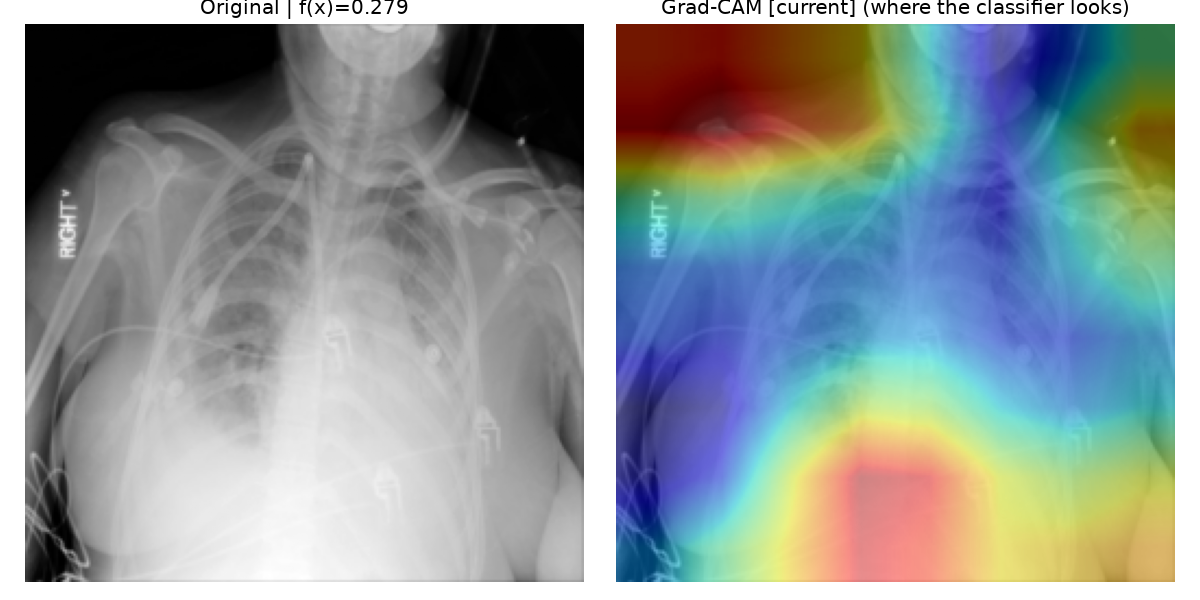
\includegraphics[width=\textwidth]{gradcam_current_0.png}
    \caption{Original classifier.}
  \end{subfigure}\hfill
  \begin{subfigure}[b]{0.48\textwidth}
    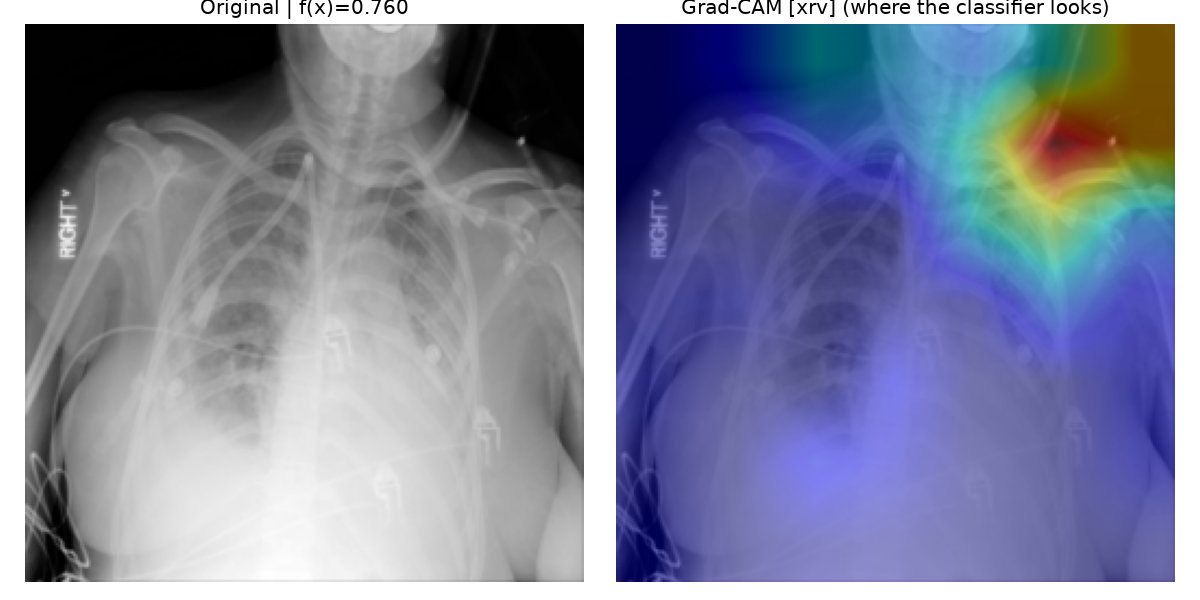
\includegraphics[width=\textwidth]{gradcam_xrv_0.png}
    \caption{TorchXRayVision DenseNet-121.}
  \end{subfigure}
  \caption[Grad-CAM localisation diagnostic]{Grad-CAM localisation diagnostic, one representative case from
  the six pairs written to \file{outputs/gradcam_check/}. This diagnostic
  motivated the replacement of the project's own ResNet-18 classifier
  (\file{checkpoint/classifier.pt}) with the pretrained TorchXRayVision
  DenseNet-121 as the guidance model.}
  \label{fig:gradcam}
\end{figure}

The same Grad-CAM implementation was subsequently promoted from a
diagnostic to a \emph{constraint}. With \texttt{USE\_GRADCAM\_MASK}, the
map is normalised at its 99th percentile, raised to a power
$\gamma = 0.75$, floored at $0.15$ and Gaussian-blurred, then used to
modulate the edit budget spatially --- so the agent may edit freely where
the classifier attends and only marginally elsewhere.

Enabling this required an ensemble-aware Grad-CAM path
(\texttt{gradcam.ensemble\_grad\_cam}). Without it, resolving the target
layer on an ensemble walks \texttt{named\_modules()} and silently returns
the \emph{first member's} feature block, producing a single-model CAM
mislabelled as the ensemble's. This is recorded in \file{config.py} as
verified behaviour rather than a suspicion.

\subsection{Sparsity Reward with Annealed Ramp}

Even after the reward rebalance, measured edit concentration --- the
share of total $|\Delta|$ carried by the top 5\% of pixels --- stood at
$0.282$ (\ntop{}) and $0.297$ (\pton{}) against a uniform baseline of
$0.05$. A concentrated core existed, but most of the edit mass sat in a
diffuse tail.

An explicit L1 sparsity reward term was added to target that tail, with
two refinements. First, it is \emph{annealed}: the weight is zero for the
first 20\% of updates, ramps linearly to its target of $2.0$ between 20\%
and 60\%, and is constant thereafter, so the policy first learns a
reliable flip and only then is pressured toward minimal edits.
Second, with \texttt{SPARSITY\_OUTSIDE\_CAM\_ONLY} the penalty is
weighted by $(1-\text{CAM})$, penalising only edit mass \emph{outside}
the attended region --- a plain L1 would also penalise the concentrated
core that the method is trying to keep.

A safeguard accompanies the ramp: validity is probed on a held-out set
every 10 updates, and the ramp freezes if it drops more than 8 points
below its pre-ramp baseline. The size of that held-out set was chosen
rather than guessed. Validity is a fraction over $N$ images, so its
resolution is $1/N$; at $N=8$ a single image moves it by 12.5 points and
the freeze would latch on noise in essentially every run. $N=24$ gives
4.2 points per image, placing the 8-point tolerance safely above the
noise floor.

\subsection{Held-Out Validation and the Move to an Ensemble}
\label{sec:heldout_method}

The most consequential finding of the internship came from questioning
the primary metric. Counterfactual Validity was being computed with the
\emph{same} classifier that produced the guidance gradient. That number is
circular: it measures how well an optimiser optimised its own objective,
not whether the resulting image depicts disease.

\file{heldout_validation.py} was written as the independent check. It
re-scores the generated counterfactuals with TorchXRayVision classifiers
that never participated in the guidance loop, and includes an agreement
control on the \emph{original} images --- so that poor transfer cannot be
dismissed as the validators simply disagreeing about the task. It is
deliberately a separate SLURM job rather than part of
\file{eval_main.py}, and caches its generated counterfactuals so that
adding a validator costs minutes rather than hours.

The results (Chapter~\ref{ch:results}, Section~\ref{sec:heldout}) were
negative, and led directly to a redesign: the guidance signal was changed
from the single RSNA model to an \textbf{ensemble} of
\texttt{densenet121-res224-rsna} and \texttt{densenet121-res224-chex}.
The reasoning is that an adversarial direction found against one model
rarely survives against an independently trained one, so requiring
consensus makes the adversarial shortcut a substantially narrower target.
The \texttt{-chex} model was chosen specifically because its 11-head
multi-task training resists the global-brightness shortcut.

This change carries a bookkeeping obligation recorded in the
configuration: any classifier in the guidance ensemble ceases to be a
valid held-out validator. The validator set was accordingly reduced to
\texttt{nih}, \texttt{mimic\_ch} and \texttt{pc}.

\section{Experimental Infrastructure}

\subsection{Smoke Tests}

\file{smoke_test.py} and \file{smoke_test_eval.py} run the training and
evaluation paths end-to-end with deliberately tiny budgets, to surface
crashes and tensor-shape errors before a 20-hour job is queued. The
training smoke test is parameterised by an \texttt{SMOKE\_ARM}
environment variable selecting \texttt{baseline} (all new flags off,
reproducing the pre-change pipeline), \texttt{mask} (Grad-CAM constraint
only) or \texttt{all} --- the same ablation arms used to attribute
behaviour changes to individual mechanisms.

\subsection{Job Monitoring}

All batch scripts declare \texttt{--mail-type=END,FAIL} with a
notification address, so job completion and failure are reported without
polling. Each script also runs \texttt{set -euo pipefail} and performs
explicit precondition checks before loading any model weights --- the
evaluation and held-out scripts verify that the expected policy
checkpoints exist, and the held-out script additionally verifies that
each validator's weights are present in the local TorchXRayVision cache,
failing in seconds rather than after three hours of generation.

One such check encodes a non-obvious detail worth recording: the
TorchXRayVision cache filename does not always match the weight
identifier. \texttt{densenet121-res224-rsna} is cached as
\texttt{kaggle-densenet121-*.pt}, because RSNA was a Kaggle competition,
so a naive existence check for \texttt{rsna-densenet121-*} fails even on
a correctly provisioned machine.

Python is invoked unbuffered (\texttt{python -u}) throughout, so that a
job's log is readable while it is still running. In a non-interactive
environment where a stalled job cannot be inspected directly, the log is
the only diagnostic channel available.

\section{Conclusion}

This chapter has described the construction of the research pipeline and
the sequence of redesigns that experimental evidence forced: a reward
function found to be 93\% flip bonus, a fidelity penalty that rewarded
the failure mode it was meant to suppress, a direction-scaling bug that
penalised preservation on the harder direction, and --- most importantly
--- a primary metric found to be circular. The next chapter reports what
the resulting system measures, and what those measurements do and do not
establish.

\chapter{Results, Discussion, and Perspectives}
\label{ch:results}

This chapter reports the measurements obtained, assesses what they do and
do not establish, and sets out perspectives for continuing the work. All
figures quoted are read directly from the serialised evaluation artefacts
in \file{checkpoints/} --- principally \file{eval_metrics.json},
\file{heldout/heldout_validation.json} and the two
\file{guidance_diagnostics_*.json} files --- rather than transcribed
from run logs.

\section{Evaluation Protocol}

Following Singla~\emph{et al.}~\cite{singla2022}, the evaluation set is
split by classifier confidence into a negative group
$X_n = \{x : f(x) < 0.2\}$ and a positive group
$X_p = \{x : f(x) > 0.8\}$, with up to $n_{\text{eval}} = 200$ images
each. The \ntop{} policy generates counterfactuals from $X_n$ toward
$c=1$; the \pton{} policy generates from $X_p$ toward $c=0$. Both use the
policy's deterministic mean action, for reproducibility.

The metric suite comprises Counterfactual Validity (CV), Fr\'echet
Inception Distance (FID)~\cite{heusel2017fid} computed in
TorchXRayVision DenseNet feature space rather than ImageNet Inception
space, a model-free Identity Preservation (IP) score, and two clinical
proxy metrics --- Cardio-Thoracic Ratio (CTR) and a costophrenic-recess
score (SCP) --- each tested with a paired $t$-test on the within-image
delta.

\subsection{Identity Preservation as a Substitute for FOP}

The reference protocol's Foreign-Object Preservation metric requires a
Fast R-CNN device detector trained on private, manually annotated data.
It is not reproducible offline, and no TorchXRayVision weight set exposes
a usable ``Support Devices'' head. FOP is accordingly reported as
\textbf{unavailable} --- it is serialised as \texttt{null} in
\file{eval_metrics.json}, not silently omitted --- and substituted by a
model-free IP score measuring the same underlying property:

\begin{itemize}[leftmargin=*]
  \item \textbf{MS-SSIM}~\cite{wang2003msssim}: multi-scale structural
        similarity between $x$ and $x_c$, capturing global anatomical
        identity.
  \item \textbf{HF-corr}: Pearson correlation between high-pass-filtered
        versions of $x$ and $x_c$. Thin, high-contrast structures ---
        tubes, leads, pacemakers --- are exactly the spatial-frequency
        content a Gaussian high-pass isolates, making this a direct proxy
        for whether such hardware survives editing.
\end{itemize}

\section{Obtained Results}

\subsection{Primary Metric Suite}

\begin{table}[h]
\centering
\caption[Primary evaluation metric suite]{Evaluation results from \file{checkpoints/eval_metrics.json},
$n_{\text{eval}} \le 200$ per group. FID is computed between each real
group and its own counterfactual set.}
\label{tab:results}
\begin{tabular}{@{}llrr@{}}
\toprule
\textbf{Metric} & \textbf{Definition} & \textbf{\ntop{}} & \textbf{\pton{}} \\
\midrule
CV        & fraction valid ($\tau = 0.8$)      & 0.995 & 0.955 \\
          & \textit{mean}                       & \multicolumn{2}{c}{0.975} \\
FID       & XRV-DenseNet features, lower better & 103.83 & 59.73 \\
IP        & MS-SSIM                             & 0.849 & 0.796 \\
IP        & HF-corr                             & 0.938 & 0.798 \\
FOP       & not computable offline              & --- & --- \\
\bottomrule
\end{tabular}
\end{table}

Counterfactual Validity is high in both directions. Section~\ref{sec:heldout}
explains why this number, taken alone, is not evidence of success.

Identity preservation is respectable and consistently better for the
\ntop{} direction (MS-SSIM $0.849$, HF-corr $0.938$) than for \pton{}
($0.796$, $0.798$), indicating that fine high-frequency structure ---
the hardware the HF-corr proxy is designed to track --- survives editing
substantially better when adding a pattern than when removing one.

The FID values are high in absolute terms. Two factors compound here.
The estimates use $N \approx 200$ samples against a 1024-dimensional
feature space, far below the sample count FID nominally requires, so
their variance is large. Beyond that, they indicate a genuine
distributional gap between generated and real radiographs that the
current training budget did not close. These should be read as
directionally informative --- \pton{} is clearly the more realistic
direction --- rather than as tightly bounded estimates.

\subsection{Clinical Proxy Metrics}

\begin{table}[h]
\centering
\caption[Clinical proxy metrics]{Clinical proxy metrics: group means $\pm$ standard deviation and
paired $t$-tests on the within-image real$\rightarrow$counterfactual delta.
Significance at $\alpha = 0.05$ marked with $^{\ast}$.}
\label{tab:clinical}
\begin{tabular}{@{}lccr@{}}
\toprule
& \textbf{Real group} & \textbf{Counterfactual} & \textbf{$\Delta$ ($t$, $p$)} \\
\midrule
\multicolumn{4}{@{}l}{\textit{\ntop{} direction ($X_n \rightarrow X_c^{n\to p}$)}}\\
CTR & $0.424 \pm 0.055$ & $0.417 \pm 0.078$ & $+0.0070$ \ ($t=1.09$, $p=0.276$) \\
SCP & $0.4794 \pm 0.0008$ & $0.4795 \pm 0.0009$ & $-0.00014$ \ ($t=-2.89$, $p=0.0042^{\ast}$) \\
\midrule
\multicolumn{4}{@{}l}{\textit{\pton{} direction ($X_p \rightarrow X_c^{p\to n}$)}}\\
CTR & $0.452 \pm 0.101$ & $0.452 \pm 0.131$ & $+0.0251$ \ ($t=2.22$, $p=0.028^{\ast}$) \\
SCP & $0.4791 \pm 0.0010$ & $0.4792 \pm 0.0011$ & $-0.00012$ \ ($t=-1.52$, $p=0.129$) \\
\bottomrule
\end{tabular}
\end{table}

The picture here is mixed and should not be overstated. Only two of the
four tests reach significance, and they are not the same two: CTR shifts
significantly in the \pton{} direction but not in \ntop{}, while SCP does
the reverse.

The CTR result is arguably the more interpretable of the two, and it is
interpretable as a \emph{success of the spatial constraint}. The
cardio-thoracic ratio is driven by the cardiac silhouette, which lies
largely outside the pure lung mask that gates editing. A system whose
background lock is working should therefore leave CTR nearly unchanged
--- which is what the small absolute magnitudes ($0.007$ and $0.025$
against group means near $0.43$) show. The SCP deltas are smaller still,
around $10^{-4}$ on a metric with a standard deviation near $10^{-3}$;
their statistical significance reflects the paired design and $n \approx 200$
rather than any clinically meaningful shift.

The honest summary is that the clinical proxy metrics are not currently
discriminative enough to support conclusions about clinical realism.
Section~\ref{sec:limitations} explains why the SCP proxy in particular
should be treated as a weak instrument.

\subsection{Qualitative Counterfactuals}

\begin{figure}[h]
  \centering
  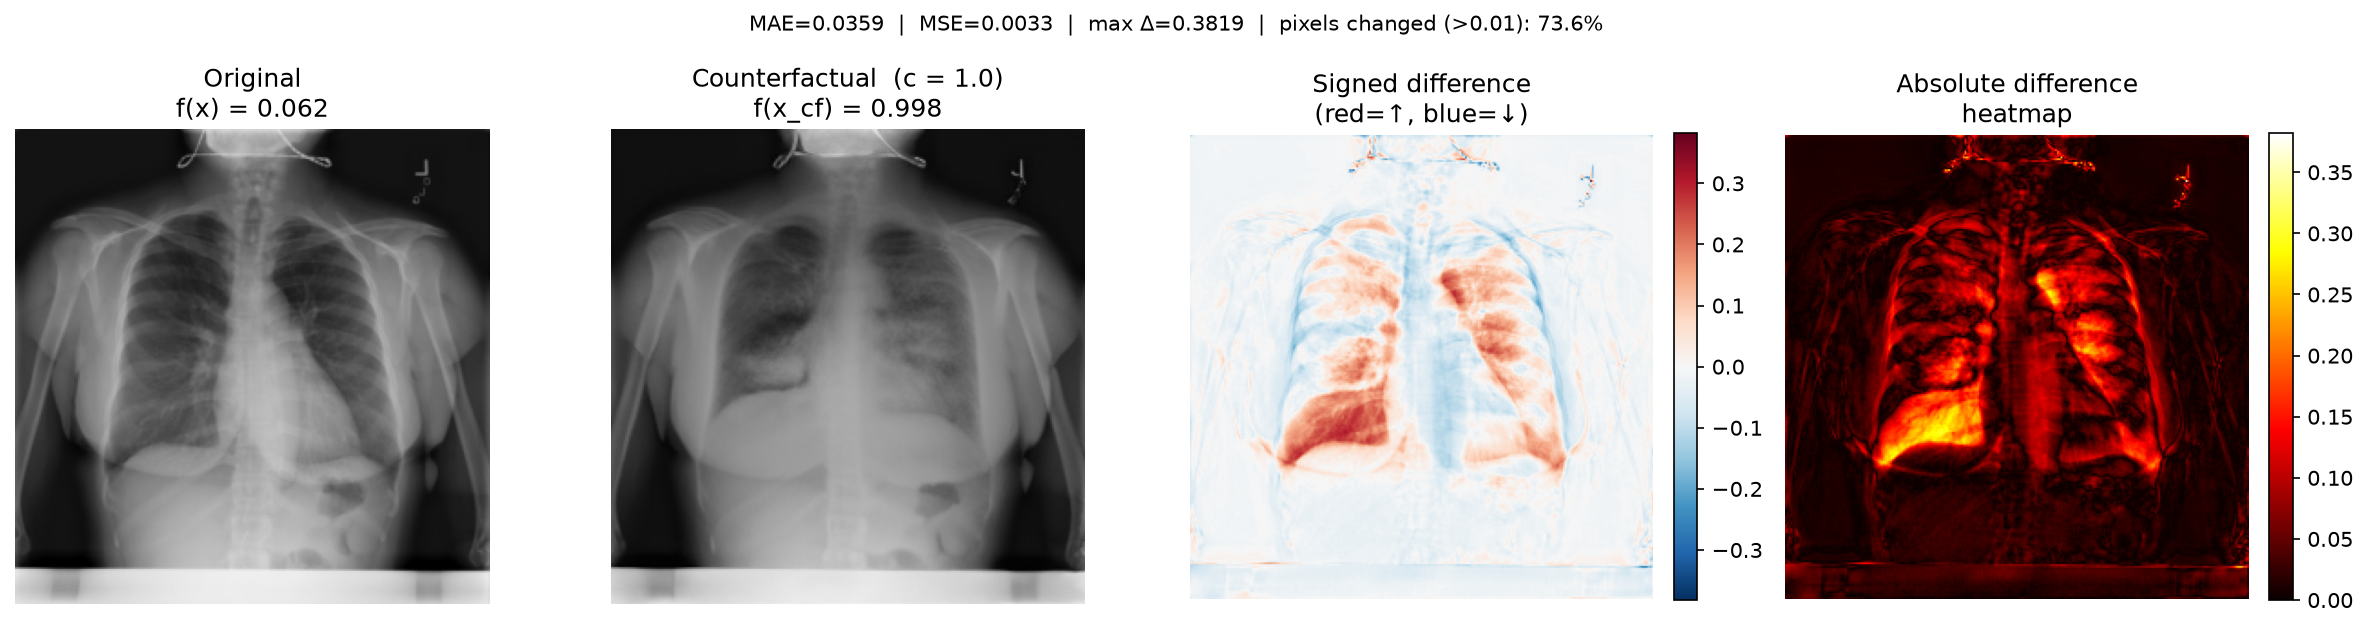
\includegraphics[width=\textwidth]{counterfactual_diff_n_to_p.png}
  \caption[Counterfactual: normal to pneumonia]{\textbf{Normal $\rightarrow$ pneumonia.} Left to right:
  original, counterfactual targeting $c=1$, signed pixel difference, and
  absolute-difference heatmap, produced by \file{src/diff_viz.py}. The
  classifier score crosses the decision boundary by a wide margin.}
  \label{fig:n2p}
\end{figure}

\begin{figure}[h]
  \centering
  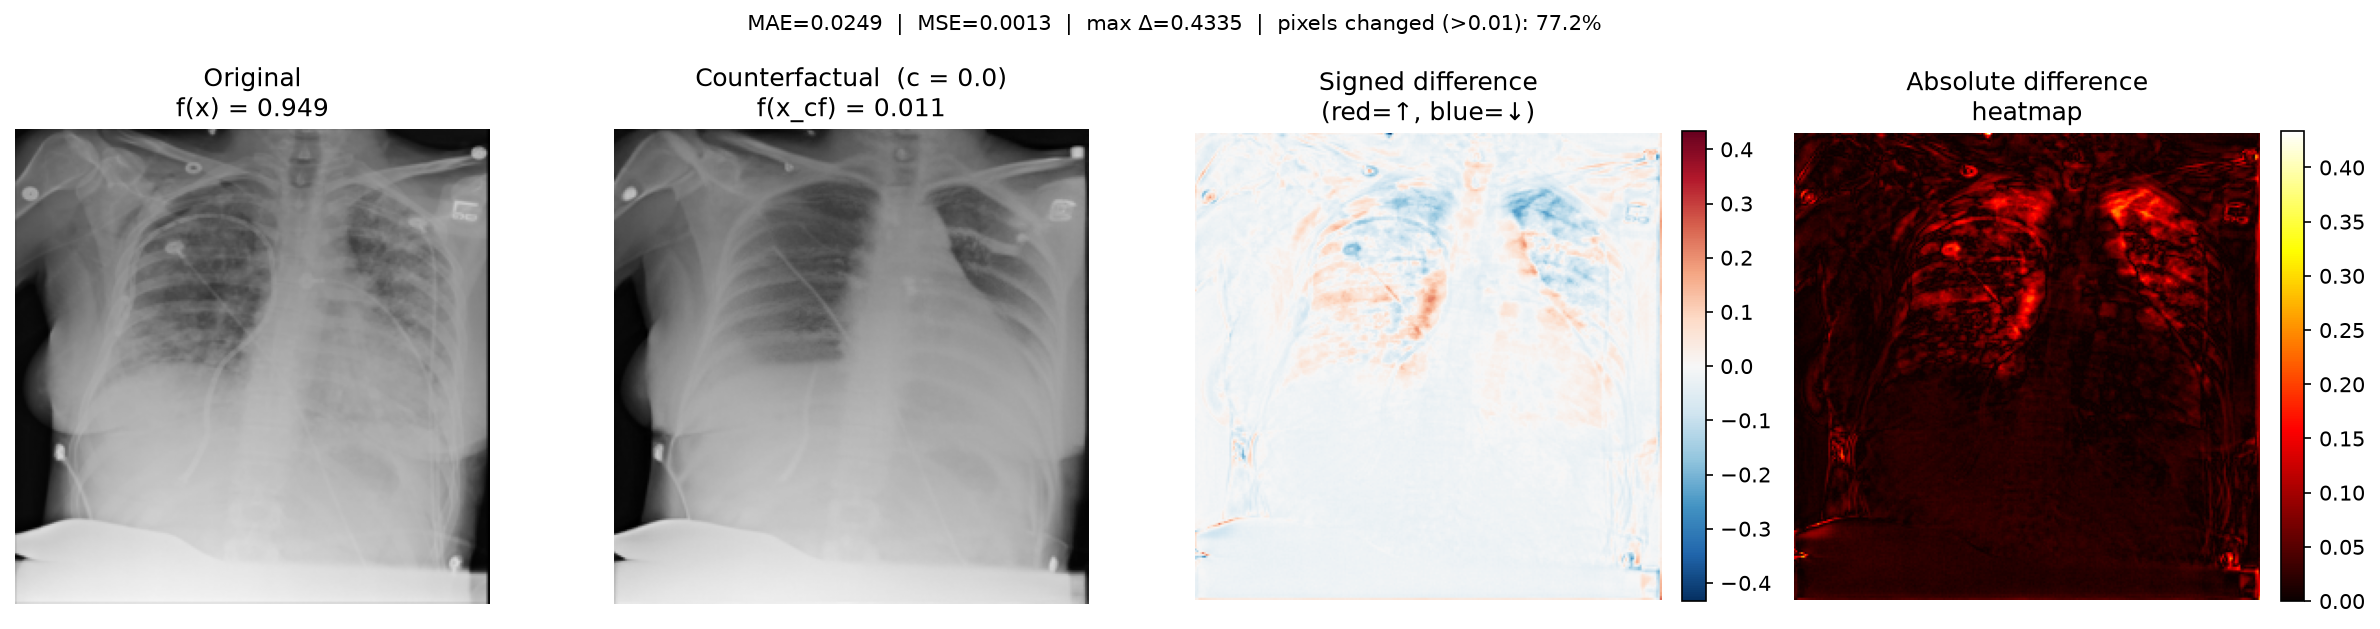
\includegraphics[width=\textwidth]{counterfactual_diff_p_to_n.png}
  \caption[Counterfactual: pneumonia to normal]{\textbf{Pneumonia $\rightarrow$ normal.} Same four-panel
  layout. Change is distributed over both lung fields, consistent with
  opacity removal, and at a lower overall magnitude than the \ntop{} case
  --- MAE $0.029$ versus $0.042$, as measured over 200 images per
  direction in \file{heldout_validation.json}.}
  \label{fig:p2n}
\end{figure}

Gross anatomical layout outside the lung field is visibly retained in
both directions, which is the qualitative signature of the background
lock holding as designed.

\subsection{Training Diagnostics}

\begin{figure}[h]
  \centering
  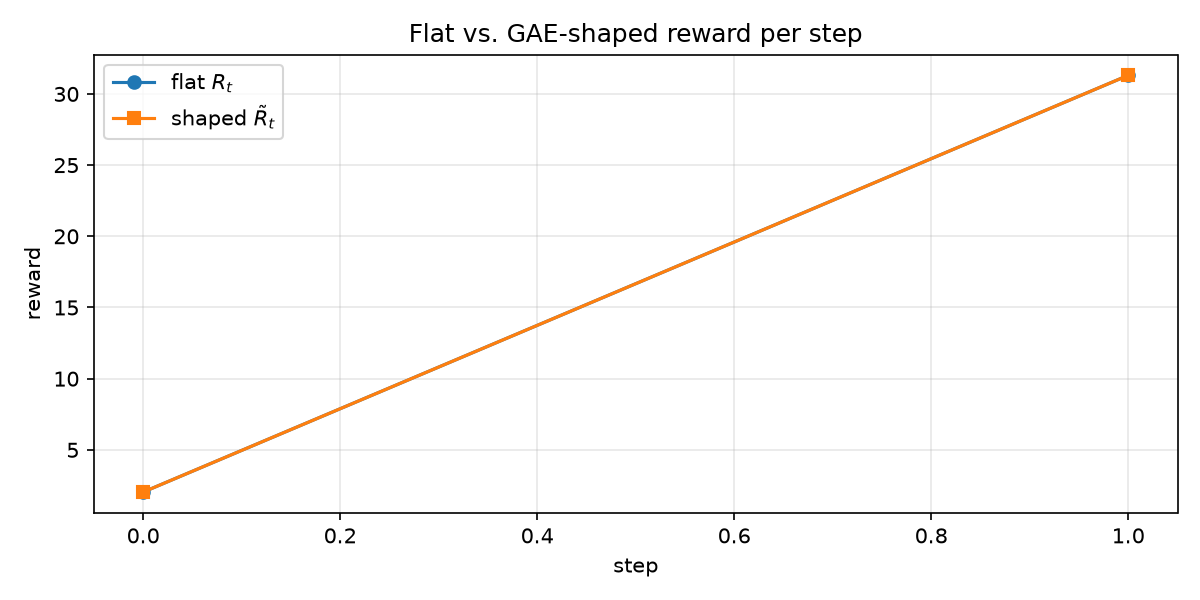
\includegraphics[width=0.72\textwidth]{reward_trace.png}
  \caption[PPO reward trace diagnostic]{Flat per-step reward $R_t$ against the GAE-shaped reward
  $\tilde R_t$ over a short post-training rollout
  (\file{factory/evaluate.py}, \texttt{plot\_reward\_trace}). The trace is
  short because this rollout reaches validity almost immediately, and the
  two curves are near-coincident --- a direct consequence of PPO's
  per-update advantage normalisation absorbing a uniform shaping term.
  This is a training-health diagnostic, not a convergence curve.}
  \label{fig:reward}
\end{figure}

The guidance diagnostics serialised alongside each policy checkpoint show
that the two directions converged to visibly different control
strategies. The \ntop{} policy settles at a guidance bias of $1.298$ ---
essentially the top of its $[0.70, 1.30]$ range --- meaning it maximally
favours classifier guidance over preservation, and suppresses
preservation to a factor of $0.771$. The \pton{} policy does the
opposite, settling at $0.701$, the bottom of the range, which
\emph{amplifies} preservation by $1.428\times$. Average reward differs
accordingly: $21.41$ for \ntop{} against $14.87$ for \pton{}.

Both policies pin their guidance bias to opposite ends of the available
range, with standard deviations below $0.006$. This near-deterministic
saturation indicates the action bound, not the policy, is the binding
constraint on this dimension --- a concrete signal that the range itself
should be widened in future work.

\section{The Held-Out Validation Result}
\label{sec:heldout}

The central experimental finding of this internship is negative, and it
concerns the interpretation of Table~\ref{tab:results}.

Counterfactual Validity there is computed with the same classifier that
generated the guidance gradient. To test whether the edits carry disease
signal rather than a perturbation tailored to that one model, job
\textbf{17649721} re-scored 200 counterfactuals per direction with two
TorchXRayVision DenseNet-121 classifiers that had never participated in
guidance.

\begin{table}[h]
\centering
\caption[Held-out validation results]{Held-out validation (\file{checkpoints/heldout/heldout_validation.json}),
$n=200$ per direction, $\tau=0.8$. Guidance classifier at generation time:
\texttt{densenet121-res224-rsna} alone. Strict CV is the fraction of
counterfactuals each validator independently judges valid.}
\label{tab:heldout}
\begin{tabular}{@{}llrrr@{}}
\toprule
\textbf{Classifier} & \textbf{Role} & \textbf{CV \ntop{}} & \textbf{CV \pton{}} & \textbf{Agreement} \\
\midrule
\texttt{-rsna}  & guidance (circular) & 0.995 & 0.885 & --- \\
\texttt{-chex}  & held out            & 0.080 & 0.000 & 0.707 \\
\texttt{-nih}   & held out            & 0.000 & 0.000 & 0.697 \\
\bottomrule
\end{tabular}
\end{table}

The gap is stark. Counterfactuals that the guidance classifier accepts
99.5\% of the time are accepted by an independent classifier at most 8\%
of the time, and in three of the four held-out cells, never. Transfer
ratios --- the fraction of the guidance model's score shift that the
validators reproduce --- are $0.205$ and $0.590$ for \ntop{} and only
$0.132$ and $0.143$ for \pton{}.

The agreement control is what makes this conclusive. On the
\emph{original}, unedited images the validators agree with the guidance
classifier around 70\% of the time ($0.697$ and $0.707$), confirming they
share a working notion of the task. They are not failing to recognise
pneumonia in general; they are failing to recognise it in these specific
generated images.

The conclusion is direct: \textbf{the \pton{} direction in particular was
not removing disease, it was fooling $f(\cdot)$.} The edits were largely
adversarial perturbations against the guidance classifier rather than
semantic changes to depicted pathology.

The edit-concentration figures recorded in the same artefact corroborate
this. Concentration --- the share of total absolute change carried by the
top 5\% of pixels --- was $0.282$ (\ntop{}) and $0.297$ (\pton{}) against
a uniform baseline of $0.05$, with 66\% and 62\% of all pixels changed
and MAE of $0.042$ and $0.029$. A focal consolidation should concentrate
well above $0.5$. These edits have a concentrated core but carry most of
their mass in a diffuse, low-amplitude tail spread over the majority of
the image --- the visual signature of an adversarial perturbation rather
than a lesion.

This result motivated the three countermeasures described in
Chapter~\ref{ch:tasks}: ensemble guidance, the Grad-CAM action-space
constraint, and the annealed sparsity reward.

\subsection{Status of the Countermeasures}
\label{sec:status}

The countermeasures are \textbf{implemented and enabled} in
\file{config.py}, and a training run under the new configuration was in
progress at the close of the internship: the most recent log
(job \textbf{17653310}) shows the ensemble classifier loading correctly
with both members, the Grad-CAM mask active, and the sparsity ramp
resolved over updates $[20, 60)$ of 100.

\textbf{A re-run of the held-out validation against the new configuration
was not completed within the internship period.} Whether ensemble
guidance, spatial constraint and sparsity pressure actually close the
transfer gap in Table~\ref{tab:heldout} is therefore an open question,
not a demonstrated result. It is the first item of future work in
Section~\ref{sec:future}.

The one measurement available from the new configuration is a caution
rather than a result: the pipeline log notes that Grad-CAM is degenerate
for one of the two ensemble members, so the constraint mask is
effectively being computed from a single member. The ensemble-aware CAM
path handles this by averaging over the remaining members instead of
failing, but it means the spatial constraint is currently weaker than the
design intends.

\section{Strengths and Limitations}

\subsection{Strengths}

\begin{itemize}[leftmargin=*]
  \item \textbf{A genuine spatial guarantee.} The background lock is a
        structural constraint rather than a penalty term. Content outside
        the lung field cannot be repainted regardless of the guidance
        gradient's behaviour, and the small CTR deltas in
        Table~\ref{tab:clinical} are consistent with it holding.
  \item \textbf{Parameter-efficient adaptation.} Domain adaptation of an
        866M-parameter generator was achieved by training 0.78\% of its
        parameters, which is what made the project feasible within a
        single-GPU budget.
  \item \textbf{Sampling control without weight modification.} The PPO
        agent never touches the diffusion weights, keeping the action
        space interpretable at 9 bounded dimensions and the learned
        policy reusable across arbitrary query images.
  \item \textbf{Falsifiable evaluation.} The project's most valuable
        output is a control that exposed its own primary metric as
        circular. The held-out validation apparatus, its agreement
        control, and the disjointness rule between guidance and validator
        sets are reusable well beyond this system.
\end{itemize}

\subsection{Limitations}
\label{sec:limitations}

\begin{itemize}[leftmargin=*]
  \item \textbf{Transfer to independent classifiers is unresolved.} This
        is the principal limitation. As of the end of the internship the
        counterfactuals demonstrably did not transfer
        (Section~\ref{sec:heldout}), and the countermeasures are
        implemented but unvalidated (Section~\ref{sec:status}).
  \item \textbf{FOP is not computable.} The reference metric requires an
        unavailable detector, and the IP substitute measures a related
        but not identical property.
  \item \textbf{SCP is a weak proxy.} It is derived from a COCO-pretrained
        YOLOv8 feature norm rather than a dedicated costophrenic-recess
        detector. Its near-zero deltas in Table~\ref{tab:clinical} should
        not be read as clinical measurements.
  \item \textbf{FID estimates are imprecise and high.} $N \approx 200$
        against a 1024-dimensional feature space gives wide error bars,
        and the absolute values indicate a real realism gap.
  \item \textbf{Compute-constrained training scale.} The episode and
        epoch budgets are documented in \file{config.py} as conservative
        placeholders sized for the available walltime, not values
        established by ablation.
  \item \textbf{Two independently trained policies.} A single
        target-conditioned policy would let the harder direction share
        representation capacity with the easier one, but requires an
        environment refactor not undertaken here.
  \item \textbf{No baseline comparison was performed.} No GAN-based
        counterfactual baseline was implemented or evaluated within this
        internship, so the system's performance is not positioned against
        prior work. This is stated explicitly because it is a real gap in
        the evaluation, not an oversight in reporting.
  \item \textbf{Single dataset, single pathology.} All results concern
        binary pneumonia classification on RSNA. Nothing here establishes
        generalisation to other pathologies, other corpora, or other
        acquisition protocols.
\end{itemize}

\section{Perspectives and Future Work}
\label{sec:future}

\begin{itemize}[leftmargin=*]
  \item \textbf{Complete the validation loop (highest priority). ---
        \emph{Resolved in Chapter~\ref{ch:closing}.}} Chapter~\ref{ch:integrity}
        showed ensemble guidance helps on no-policy arms; Chapter~\ref{ch:closing}
        retrains both directional policies from scratch under it and
        re-scores them against \texttt{\{nih, pc, mimic\_ch\}} (the leak-free
        validator set, since \texttt{chex} is now a guidance member). Mean
        transfer improves on both directions ($0.230\to0.282$ \ntop{},
        $0.146\to0.293$ \pton{}), but \texttt{nih}'s \ntop{} ratio does not
        ($0.080\to0.046$) --- a partial, not complete, closure of the gap.
  \item \textbf{Resolve the trained-vs-random paired significance test. ---
        \emph{Resolved in Chapter~\ref{ch:closing}.}}
        Table~\ref{tab:lhr_arms} in Chapter~\ref{ch:integrity} shows trained
        editing toward a higher LHR lift than random ($2.293$ vs.\ $2.204$)
        at the group level; \S\ref{sec:closing_significance} runs
        \file{paired\_arm\_test.py}'s per-image paired test on the same 183
        images and finds the gap survives ($p=0.012$) at a small effect size
        ($d=0.19$).
  \item \textbf{Run the ablation arms.} The \texttt{SMOKE\_ARM}
        infrastructure (\texttt{baseline} / \texttt{mask} / \texttt{all})
        is already in place to attribute any improvement to the
        individual mechanisms rather than to their combination.
  \item \textbf{Diagnose why the Grad-CAM constraint hurts lesion
        targeting.} Chapter~\ref{ch:integrity} found the Grad-CAM mask
        (ARM~2) measurably \emph{lowers} LHR lift relative to baseline,
        both alone and combined with ensemble guidance --- the opposite of
        its intended effect. With Grad-CAM degenerate for one ensemble
        member, the spatial constraint may be operating on an unreliable
        mask; diagnosing that is now a more concrete, more urgent version
        of this item than when it was first identified.
  \item \textbf{Widen the guidance-bias action range.} Both policies
        saturate at opposite ends of $[0.70, 1.30]$ with near-zero
        variance, indicating the bound rather than the policy is binding.
  \item \textbf{Increase evaluation sample size.} The single most direct
        lever on FID precision.
  \item \textbf{Implement a baseline comparison.} A GAN-based
        counterfactual generator evaluated under an identical protocol
        would place these results in context.
  \item \textbf{Unify the two policies.} A single target-conditioned
        policy with randomised per-episode target would be
        architecturally cleaner and would let the harder \ntop{}
        direction borrow capacity from the easier one.
  \item \textbf{Broaden scope.} Extending beyond binary pneumonia to
        multi-pathology counterfactuals, and to a second corpus, would
        test whether any of this generalises.
\end{itemize}

\section{Conclusion}

This chapter has reported the system's measured performance and
subjected it to an independent control that substantially qualifies it.
High counterfactual validity against the guidance classifier proved not
to survive contact with classifiers that never guided it. The
countermeasures this motivated are built and running, but their
effectiveness is not yet established. The following general conclusion
reflects on what the internship produced and what it taught.

\chapter{Additional Work: Extending to a Second Domain}
\label{ch:breast}

Everything reported up to this point concerns a single dataset and a single
pathology: binary pneumonia classification on RSNA chest radiographs. This
short chapter documents work that sits outside the six work packages of
Chapter~\ref{ch:context} --- a self-initiated extension, undertaken once the
core RSNA pipeline and its held-out-validation apparatus were in place, to
test whether the method and, more importantly, its \emph{evaluation
discipline} generalise beyond chest radiography at all. It should be read as
exactly that: additional, exploratory work, reported with the same honesty
as Chapter~\ref{ch:results}, not as a second fully-validated result standing
alongside the main one.

\section{Motivation}

Section~\ref{sec:heldout} established the internship's central lesson: a
counterfactual system can report near-perfect validity against the
classifier that guided it while having learned almost nothing about the
target pathology. That lesson is only as strong as its generality. A single
success --- or, here, a single negative result --- on one dataset, one
modality and one pretrained model zoo leaves open the possibility that the
finding was an artefact of RSNA, of TorchXRayVision, or of pneumonia
specifically.

Mammography was chosen as the second domain precisely because it shares as
little as possible with the first. It is a different imaging modality, it
has no representation at all in TorchXRayVision's eighteen pathology
labels, and its natural binary task --- malignant versus benign lesion ---
is semantically different from RSNA's healthy-versus-diseased framing, as
discussed in Section~\ref{sec:breast_semantics}. If the pipeline's
architecture and its habit of distrusting its own validity number survive a
change this large, that is much stronger evidence than a second run on a
second chest-radiograph corpus would have been.

\section{A Domain-Registry Architecture}

Before this extension, three things that logically belong together were
scattered across unrelated parts of the system: the dataset and its label,
the pathology head the classifier guidance targets, and which clinical
metrics are even meaningful for that pathology. Changing the dataset without
also changing the other two silently produces nonsense --- guidance toward
the wrong disease, or a cardio-thoracic ratio reported for an anatomy that
has no heart in frame.

A domain-registry abstraction was introduced to bind all three together,
with a set of optional construction hooks that a domain may override when
the TorchXRayVision-shaped defaults --- an XRV classifier head, a PSPNet
segmenter, CTR/SCP as the clinical metrics --- do not apply. Left unset, a
domain behaves exactly as the original single-dataset pipeline did, which
is what keeps the RSNA domain's behaviour byte-identical to the
pre-refactor version. Adding a new dataset is then a self-contained new
domain module plus a one-line registration, rather than an edit threaded
through ingestion, guidance and evaluation code.

\section{What Mammography Required Rebuilding}

Almost nothing about the TorchXRayVision-based guidance stack survives the
move to mammography, because that whole stack --- the pathology classifier,
the PSPNet lung/heart segmenter, and the FID feature extractor --- has no
breast equivalent. The mammography domain therefore supplies its own
version of every frozen component the RSNA pipeline was able to borrow for
free.

\subsection{A classifier trained from scratch}

A dedicated training procedure builds $f(\cdot)$ for this domain, since no
pretrained breast-malignancy head exists in the model zoo used elsewhere in
this project. Three backbones are trained --- a DenseNet-121, an
EfficientNet-B0~\cite{tan2019efficientnet}, and a ResNet-18; the first two
are registered as the guidance ensemble and the third is held back as the
independent validator, mirroring the guidance/validator split described in
Section~\ref{sec:heldout_method} for the chest domain. A gating step
applies a hard floor (minimum acceptable AUC of $0.65$) against each
backbone's saved validation AUC before any of them is allowed to guide
generation, failing explicitly rather than proceeding with a near-chance
classifier.

Two details of how that played out in practice matter for reading
Section~\ref{sec:breast_results}, and neither is visible from the design
above. First, the runs that produced the counterfactuals reported here were
made with \texttt{USE\_GUIDANCE\_ENSEMBLE = False}, so $f(\cdot)$ during
generation was the \emph{single} DenseNet-121 (validation AUC $0.796$), not
the two-model ensemble; the transfer denominator in
Table~\ref{tab:breast_transfer} is that single model accordingly. Second,
those saved validation AUCs are themselves optimistic: the trainer keeps the
best-scoring epoch and reports its score on the same fold it selected on, so
$0.796$ is a maximum over thirty epochs rather than a clean estimate. The
validators trained in Section~\ref{sec:breast_results} use nested folds to
avoid that, which is part of why their honest AUCs look lower.

The split is taken at the \emph{patient} level, not the image level. CBIS-DDSM
contains up to four images per patient (left/right breast, CC/MLO view) plus
one row per lesion; a random image-level split would place the same breast
in both train and validation and report a memorisation score as an AUC.

What that patient-level split does \emph{not} do --- and this is the flaw
Section~\ref{sec:breast_results} turns on --- is separate the three backbones
from \emph{each other}. All three take the same split, so the ``held-back''
ResNet-18 trains on precisely the images the guidance model trains on. It is
architecturally independent and statistically not independent at all.

\subsection{Two segmenters instead of one}

The chest pipeline's single PSPNet segmenter conflated two roles that
mammography must separate:

\begin{itemize}[leftmargin=*]
  \item An analytic (not learned) anatomy segmenter producing
        breast/pectoral/dense-tissue masks, used to gate the background
        lock exactly as the lung mask does for RSNA.
  \item A learned lesion segmenter, a U-Net~\cite{ronneberger2015unet}
        trained on CBIS-DDSM's shipped region-of-interest masks. It is
        deliberately excluded from the guidance loop, so that the
        clinical metrics computed from it stay independent of the edits
        they are measuring --- the same independence principle that
        motivated held-out validation in the first place.
\end{itemize}

\subsection{A new clinical metric suite}

CTR and SCP, the chest domain's clinical proxy metrics, have no meaning
here: there is no heart or costophrenic recess in a mammogram. Four
mammography-specific metrics were added instead.

\begin{itemize}[leftmargin=*]
  \item \textbf{LLR (Lesion Load Ratio)} --- lesion area over breast area,
        the structural analogue of CTR. Benign$\to$malignant edits are
        expected to raise it; malignant$\to$benign edits to lower it.
  \item \textbf{MSI (Margin Spiculation Index)} --- normalised boundary
        complexity (perimeter$^2$ / $4\pi\cdot$area) of the segmented
        lesion's largest component. Margin morphology is the single most
        load-bearing malignancy sign in mammography, and CBIS-DDSM labels it
        directly (spiculated/ill-defined versus circumscribed margins),
        which makes MSI \emph{calibratable on real images} in a way SCP
        never was. A dedicated calibration check is the gate: MSI must
        separate spiculated from circumscribed lesions on ground-truth
        images before it may be reported as evidence about counterfactuals
        at all. This calibration procedure was written and is part of the
        delivered pipeline, but was not run to completion within the time
        available for this additional work, so the MSI numbers in
        Section~\ref{sec:breast_results} should be read as provisional
        pending that gate.
  \item \textbf{BDC (Breast Density Contrast)} --- mean intensity of the
        segmented dense (fibroglandular) tissue. This one is a diagnostic
        rather than a success criterion, purpose-built to catch a specific
        failure this project had already seen once, on RSNA: an early
        policy version reported a Counterfactual Validity of $0.975$ while
        changing 73.6\% of all pixels at a mean absolute error of $0.036$
        --- a diffuse global brightness wash that moved the classifier
        without editing any anatomy. The mammography signature of the same
        failure is a large BDC shift paired with a flat LLR: the generator
        brightened or darkened the whole breast rather than altering a
        lesion. Section~\ref{sec:breast_results} reports exactly this
        pattern.
  \item \textbf{MOP (Marker/clip Preservation)} --- the mammography
        counterpart of FOP, and, unlike FOP, computable offline: surgical
        clips and skin markers are small, saturated, high-contrast metal
        objects that a simple blob detector can find without a trained
        model, sidestepping FOP's dependency on a device detector that does
        not exist for this project.
\end{itemize}

\section{Dataset and Label Semantics}
\label{sec:breast_semantics}

CBIS-DDSM (Curated Breast Imaging Subset of DDSM)~\cite{lee2017cbisddsm} is
retrieved from a public Kaggle mirror by the same provisioning step used
for RSNA. It ships 3{,}568 mass and calcification lesion
\emph{rows}, pooled across both abnormality types. Those rows are one per
\emph{lesion}, and a mammogram may carry several, so the dataset the loader
actually yields is one row per image: \textbf{2{,}857 full mammograms from
1{,}460 patients, 1{,}277 malignant against 1{,}580 benign or
benign-without-callback} (44.7\% positive) --- a considerably less skewed
split than RSNA's 22.5\% positive rate. Earlier drafts of this chapter
quoted the lesion-row figures (``$\sim$3{,}500'', ``1{,}400 / 2{,}100'') as
if they were image counts; the image-level numbers above are the ones every
result in this chapter is computed over.

One property of the dataset changes what the resulting counterfactuals mean.
CBIS-DDSM is a curated subset of \emph{lesion} cases: every image in it
contains an abnormality, and there are no normal mammograms at all. The
binary label is therefore \textbf{malignant versus benign}, not
healthy versus diseased, and the two PPO directions are
benign$\to$malignant and malignant$\to$benign. This is stated explicitly
because it is easy to misread: a reader carrying over the chest framing
might read a successful malignant$\to$benign edit as ``the model removed
the cancer,'' when what it actually claims is the narrower, weaker
statement that the generator made an already-present lesion look benign to
the classifier.

\section{Results}
\label{sec:breast_results}

The trained system was evaluated with the same protocol as
Chapter~\ref{ch:results}: groups split by classifier confidence
($n_{\text{eval}} \le 200$ per direction), deterministic mean-action policy
rollouts.

\begin{table}[h]
\centering
\caption[Breast-domain primary metrics]{Primary evaluation metrics, mammography domain. FID compares each
counterfactual set against its own real target group. The CV row and the
held-out transfer row appear together deliberately: CV is measured against
the classifier that guided generation, and is not interpretable without an
independence check beside it. Transfer is
$\Delta_{\text{validator}}/\Delta_{\text{guidance}}$; see
Table~\ref{tab:breast_transfer} for per-validator confidence intervals.}
\label{tab:breast_results}
\begin{tabular}{@{}llrr@{}}
\toprule
\textbf{Metric} & \textbf{Definition} & \textbf{benign$\to$malig.} & \textbf{malig.$\to$benign} \\
\midrule
CV   & fraction valid ($\tau = 0.8$), \emph{vs.\ the guidance model} & 1.000 & 1.000 \\
     & \textit{mean}                       & \multicolumn{2}{c}{1.000} \\
\addlinespace
\textbf{Transfer} & \textbf{independent validators, mean} & \textbf{0.066} & \textbf{0.056} \\
     & \quad resnet18-heldout (AUC 0.723)  & 0.116 & 0.032 \\
     & \quad effnet-b0-heldout (AUC 0.693) & 0.017 & 0.080 \\
     & \quad \textit{same-corpus validator (AUC 0.988)} & \textit{0.476} & \textit{0.327} \\
\addlinespace
FID  & breast-domain features, lower better & 163.6 & 193.8 \\
IP   & MS-SSIM                             & 0.891 & 0.886 \\
IP   & HF-corr                             & 0.932 & 0.946 \\
EditConcentration & top-5\% pixel mass share (uniform baseline $0.05$) & 0.367 & 0.332 \\
     & fraction of pixels changed          & 38.2\% & 40.6\% \\
MOP  & marker preservation                 & 0.930 & 0.872 \\
\bottomrule
\end{tabular}
\end{table}

\begin{table}[h]
\centering
\caption[Breast-domain clinical proxy metrics]{Mammography clinical proxy metrics: mean within-image delta and
paired $t$-test. Significance at $\alpha=0.05$ marked with $^{\ast}$.}
\label{tab:breast_clinical}
\begin{tabular}{@{}lrr@{}}
\toprule
\textbf{Metric} & \textbf{$\Delta$ benign$\to$malig.\ ($t$, $p$)} & \textbf{$\Delta$ malig.$\to$benign ($t$, $p$)} \\
\midrule
LLR & $+0.00014$ ($t=0.04$, $p=0.970$) & $-0.00107$ ($t=-0.34$, $p=0.732$) \\
MSI & $-0.082$ ($t=-1.39$, $p=0.165$)  & $-0.055$ ($t=-1.68$, $p=0.094$) \\
BDC & $+0.0014$ ($t=0.29$, $p=0.773$)  & $+0.0154$ ($t=2.46$, $p=0.015^{\ast}$) \\
\bottomrule
\end{tabular}
\end{table}

\begin{table}[h]
\centering
\caption[Breast-domain held-out transfer]{Held-out transfer ratio by validator and direction,
$n=200$ per group. Percentile bootstrap over 10{,}000 resamples, with
numerator and denominator resampled jointly so the within-image pairing is
preserved. Verdict thresholds as in Section~\ref{sec:heldout}: below $0.15$
adversarial, below $0.5$ partial. AUC is measured on the 400 real eval
originals (190 benign / 210 malignant) against radiologist pathology; $\rho$
is rank agreement with the guidance model on those same unedited images,
which separates ``disagrees about the edit'' from ``disagrees about
everything''.}
\label{tab:breast_transfer}
\resizebox{\textwidth}{!}{%
\begin{tabular}{@{}llrrrr@{}}
\toprule
\textbf{Validator} & \textbf{Independence} & \textbf{AUC} & \textbf{$\rho$} & \textbf{benign$\to$malig.} & \textbf{malig.$\to$benign} \\
\midrule
\multicolumn{6}{@{}l}{\textit{Independent and competent --- these are the result}} \\
resnet18-heldout   & patient-disjoint & 0.723 & $+0.385$ & $0.116$ $[0.097, 0.136]$ & $0.032$ $[0.017, 0.047]$ \\
effnet-b0-heldout  & patient-disjoint & 0.693 & $+0.370$ & $0.017$ $[-0.011, 0.044]$ & $0.080$ $[0.057, 0.103]$ \\
\textbf{mean}      &                  &       &          & $\mathbf{0.066}$ & $\mathbf{0.056}$ \\
\midrule
\multicolumn{6}{@{}l}{\textit{Reported for contrast --- neither is an independence check}} \\
resnet18-cbis      & same train fold  & 0.988 & $+0.826$ & $0.476$ $[0.427, 0.526]$ & $0.327$ $[0.282, 0.373]$ \\
resnet18-cmmd      & external corpus  & 0.507 & $+0.055$ & $0.091$ $[0.071, 0.111]$ & $0.052$ $[0.034, 0.069]$ \\
effnet-b0-cmmd     & external corpus  & 0.499 & $-0.000$ & $-0.006$ $[-0.019, 0.007]$ & $0.095$ $[0.084, 0.107]$ \\
\bottomrule
\end{tabular}%
}
\end{table}

Figures~\ref{fig:breast_n2p} and~\ref{fig:breast_p2n} show representative
qualitative examples for each direction.

\begin{figure}[h]
  \centering
  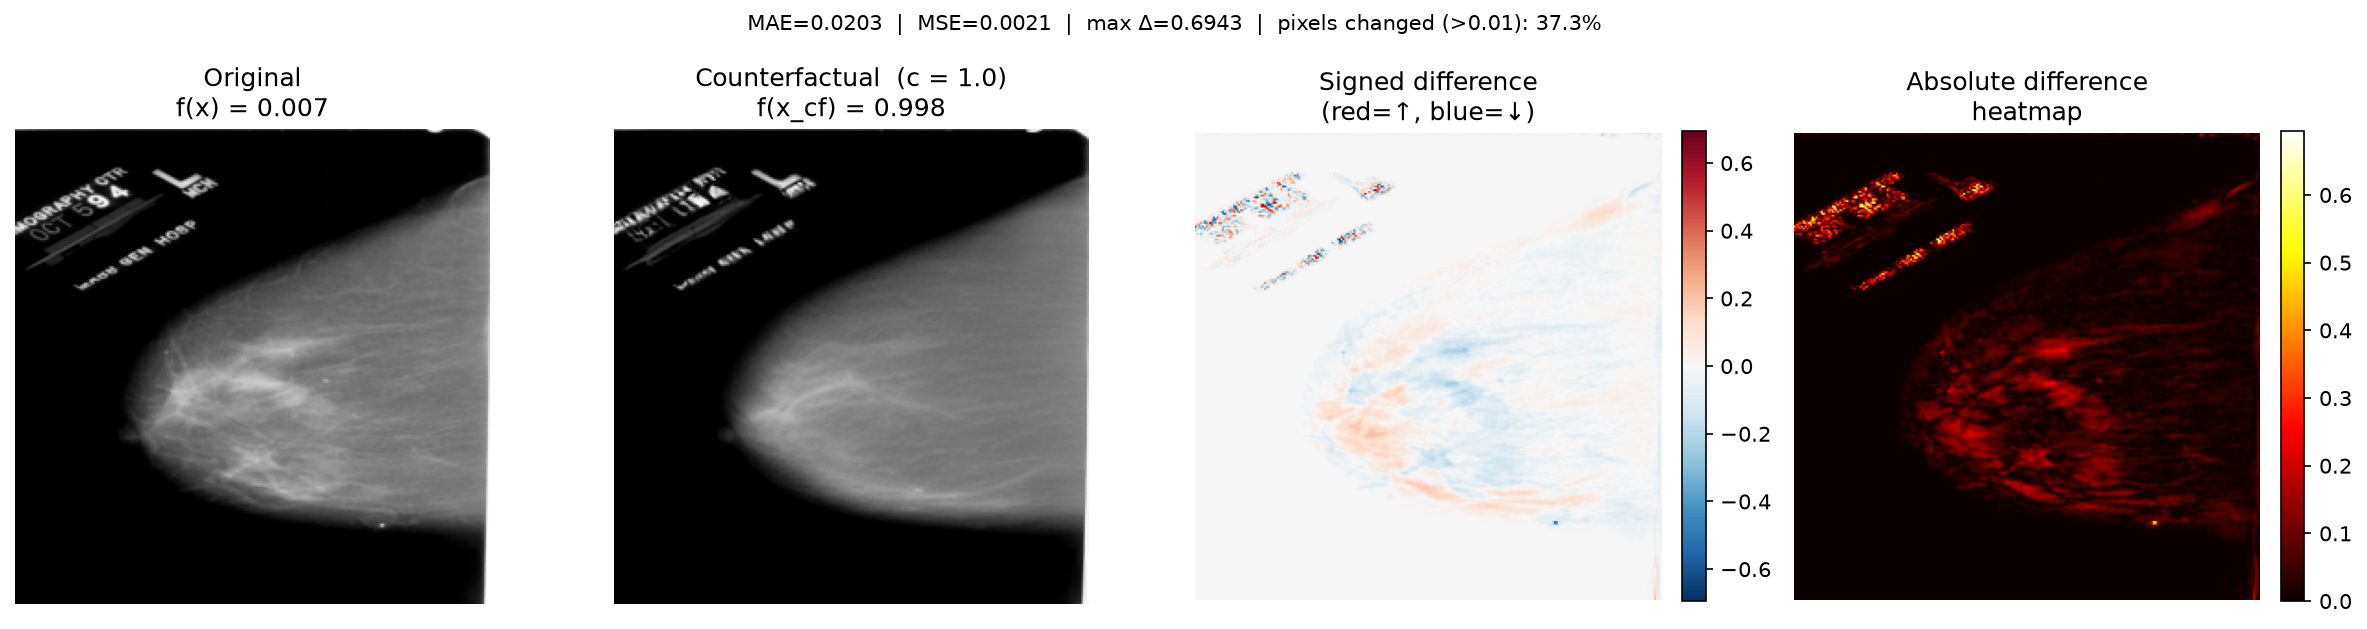
\includegraphics[width=\textwidth]{counterfactual_diff_n_to_p_breast.png}
  \caption[Breast counterfactual: benign to malignant]{\textbf{Benign $\rightarrow$ malignant.} Original, counterfactual
  targeting the malignant class, signed pixel difference, and
  absolute-difference heatmap, on the mammography domain.}
  \label{fig:breast_n2p}
\end{figure}

\begin{figure}[h]
  \centering
  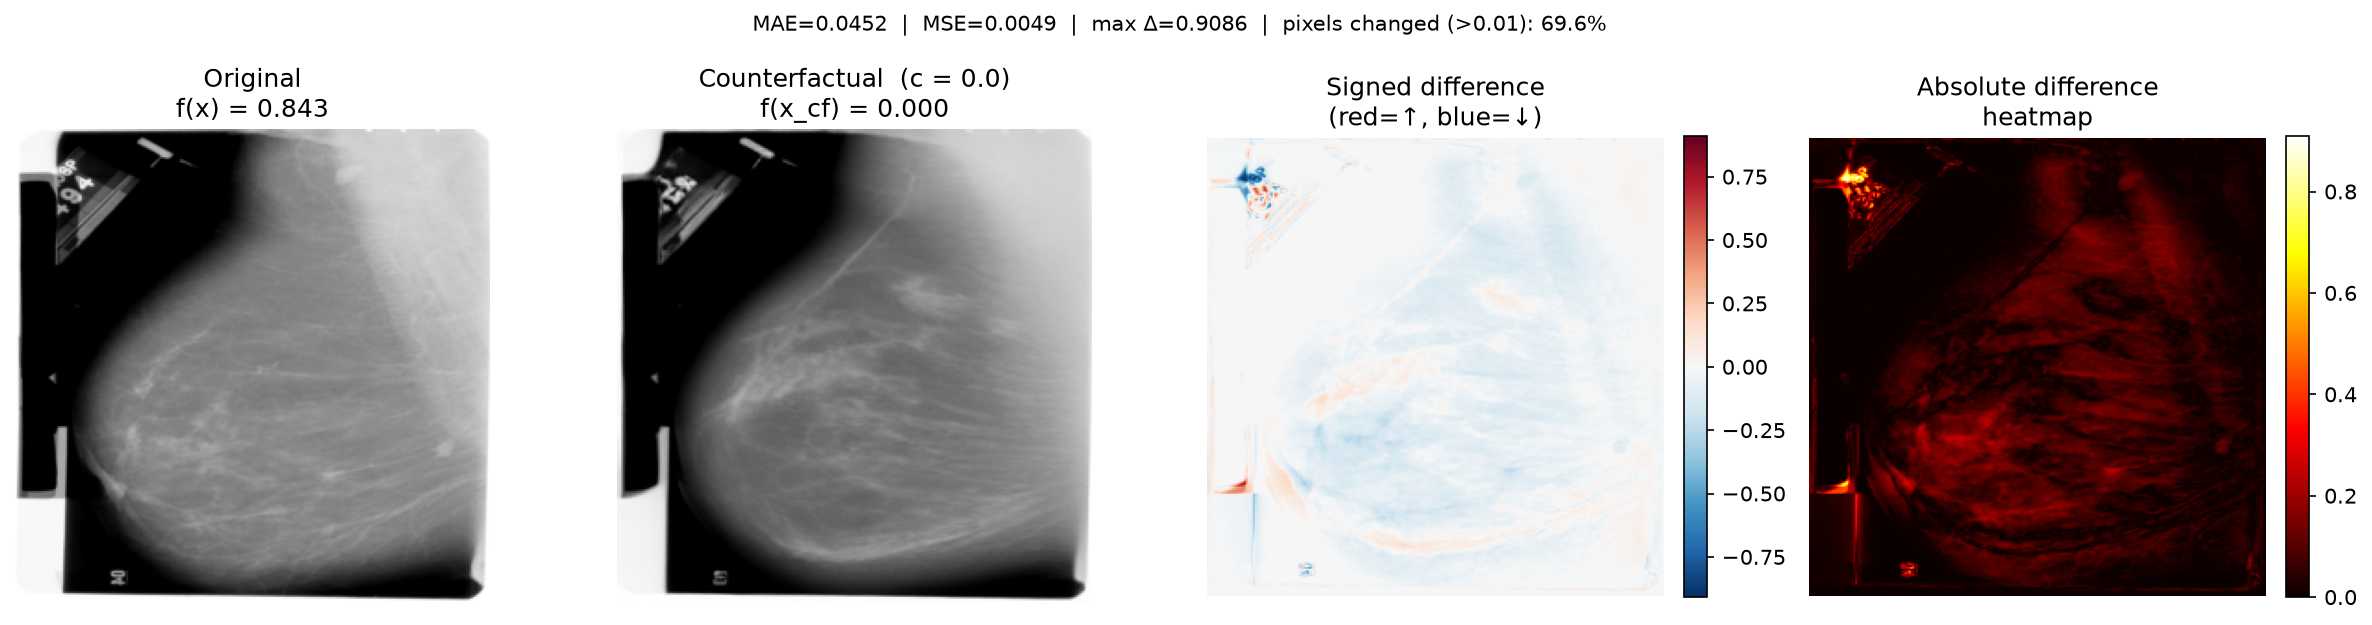
\includegraphics[width=\textwidth]{counterfactual_diff_p_to_n_breast.png}
  \caption[Breast counterfactual: malignant to benign]{\textbf{Malignant $\rightarrow$ benign.} Same four-panel layout.}
  \label{fig:breast_p2n}
\end{figure}

The guidance diagnostics recorded alongside each policy checkpoint (a
20-episode probe) show the same kind of directional specialisation
observed on RSNA: the benign$\to$malignant policy settles at a higher
guidance bias (mean $0.980$, $3.45$ refinement passes on average, average
reward $8.53$) than the malignant$\to$benign policy ($0.790$, $3.20$
passes, average reward $5.10$), indicating the two directions again
learned visibly different control strategies rather than converging to a
shared, direction-agnostic schedule.

\subsection{Reading These Numbers Honestly}

Three things in these tables should stop a reader before they are taken as a
mammography success story.

\textbf{The CV number is exactly the shape of the number that misled the
project once already, and the held-out column beside it says so.} A mean
Counterfactual Validity of $1.000$ against the guidance classifier is,
superficially, an even stronger result than RSNA's $0.975$.
Section~\ref{sec:heldout} showed that a comparably high number computed
against a guidance classifier collapsed to at most 8\% under genuinely
independent validators. The same thing happens here, and harder: against
validators that never saw the guidance model's training data and never saw
one of the 400 images they score, the counterfactuals reproduce a mean
$6.6\%$ (benign$\to$malignant) and $5.6\%$ (malignant$\to$benign) of the
guidance model's own score shift. All four bootstrap intervals in
Table~\ref{tab:breast_transfer} lie wholly below the $0.15$ adversarial
threshold, the widest reaching only $0.136$, so at $n=200$ per group this is
not a small sample failing to resolve an effect --- the adversarial regime is
positively established. In one direction the EfficientNet validator's
interval, $[-0.011, 0.044]$, contains zero, meaning no detectable malignancy
signal at all. The chest domain's \emph{worst} arm transfers at
$0.230/0.146$; mammography is more adversarial than any RSNA arm, not less.

\textbf{The validator this domain reserved was never an independence check,
and the gap shows what that was worth.} The plan in
Section~\ref{sec:heldout_method} was sound --- train three backbones, guide
with two, hold one back --- and
\texttt{DomainProfile.validate()} does enforce that the held-back model never
appears in the guidance fields. But all three were trained by
\texttt{train\_breast\_classifier.py} on \emph{one} patient-level split
(\texttt{seed}~0, \texttt{val\_frac}~0.2), so
\texttt{resnet18-breast-cbis} shares every training image with the model it
was meant to check --- and, because the eval groups were drawn from the whole
corpus, it had also been fit on 336 of the 400 eval images (84\%, spanning
304 of 362 patients). Its AUC on those images is $0.988$, against $0.723$ and
$0.693$ for validators that have not seen them: that is memorisation, not
accuracy. Reported as this domain's independence check it would have read
$0.476/0.327$ --- ``partial'' on this project's own scale, four to ten times
the honest figure. The check compared model \emph{identity}; nothing compared
training \emph{data}. That is a general lesson, not a mammography one.

\textbf{The BDC/LLR pairing reached the same conclusion first, and that
convergence is the strongest part of this result.} In the
malignant$\to$benign direction, BDC shifts significantly ($t=2.46$,
$p=0.015$) while LLR --- the metric that would move if a lesion were actually
shrinking or disappearing --- does not ($p=0.732$). That is precisely the
pattern BDC was designed to catch: a diffuse change in overall breast density
large enough to move the classifier, occurring while the segmented lesion's
relative size is statistically unchanged. Read together with an
edit-concentration figure well below what a focal, lesion-confined edit would
produce (0.33--0.37 against a uniform baseline of $0.05$, with 38--41\% of
all pixels changed), the diffuse-edit reading was already the defensible one.

The held-out transfer ratio is a second instrument with nothing
methodological in common with the first --- an independently trained
classifier rather than a statistic derived from a segmentation mask --- and
it agrees. That agreement is not a coincidence but a prediction borne out: a
diffuse density wash that moves a density-sensitive classifier without
altering the lesion is exactly the kind of edit a classifier trained on
different patients would fail to follow. Either result alone would be
suggestive; two unrelated measurements converging is what makes the reading
defensible.

\subsection{What Would Have to Be True for This to Be Wrong}

Three limits are worth stating plainly, because none of them is dissolved by
the result above.

\textbf{The independent validators are competent, not strong.} At AUC
$0.69$--$0.72$ they set a floor on how much real signal an edit must carry
before it registers, and a subtle but genuine lesion change could fall below
it. The finding is that a large adversarial component is present, not that
the disease signal is exactly zero. That ceiling is a data limit rather than
a modelling one: the only CBIS-DDSM patients no guidance backbone was fit on
number 292, and after removing every patient appearing in the eval groups the
training pool is 234 patients / 432 images, against the guidance model's
2{,}290.

\textbf{The external-corpus check was attempted and failed its own sanity
gate, and both of its AUCs are worth reporting rather than just the failing
one.} A validator trained on CMMD --- different country, different scanner
generation, no possible patient overlap --- would in principle have been the
strongest independence claim available. On its \emph{own} held-out CMMD
patients it reaches out-of-fold AUC $0.624$ (ResNet-18) and $0.635$
(EfficientNet-B0): meaningfully above chance, but already below this
project's $0.65$ floor on its native data, before CBIS-DDSM enters the
picture at all. Scored on real CBIS-DDSM images it collapses further, to
AUC $0.507$ and $0.499$ --- indistinguishable from chance --- with rank
agreement $\rho = +0.055$ and $\rho = -0.000$ against the guidance model on
the unedited originals. The scores are not degenerate (std $0.108$, a
roughly unimodal spread from $0.18$ to $0.82$), so this is not a broken
forward pass; the label mapping and the pixel-preprocessing pipeline are
byte-identical to CBIS-DDSM's. What differs is framing: CMMD's mirror ships
pre-cropped lesion patches (34.5\% near-black background) against
CBIS-DDSM's full mammograms (54.7\%), and the classifier appears to have
keyed on something in that framing rather than on transferable malignancy
signal. This was already a weak validator on its own corpus, and the drop
to chance on a different one is a domain-shift failure layered on top of a
mediocre starting point, not a strong classifier undone by nothing but
format. Either way its transfer ratios are \emph{uninterpretable} and
excluded from the mean: a classifier that cannot tell real malignant from
real benign would not follow a genuine disease edit either, so a low ratio
from it is evidence about the validator, not about the counterfactuals ---
which is why every validator here is gated on AUC before its ratio is
read at all.

\textbf{Disjointness holds at two levels of three, and the third is
arithmetically out of reach.} The ideal validator would have touched none of
the guidance model's training data, none of its validation data, and none of
the PPO rollout pool. These validators clear the first and score images they
have never seen. They do not clear the other two, and it is worth being exact
about why.

They are trained on the guidance models' \emph{validation} fold --- the 292
patients left over from the 1{,}168 the guidance model was fit on, minus the
eval-group patients, leaving 234. CBIS-DDSM contains 1{,}460 patients and the
split is 1{,}168 / 292, so excluding both folds leaves precisely zero
patients: within this corpus there is no third partition to draw from. What
that fold touched is narrow --- the guidance checkpoint was the best-scoring
epoch on it, so those images influenced \emph{which epoch was frozen}, not
what the weights learned. And the bias it introduces runs against the finding
rather than toward it: a validator sharing images with the guidance model's
selection criterion should agree with it \emph{more}, inflating transfer, not
suppressing it. The measured $0.066/0.056$ is therefore conservative.

They are also not disjoint from the PPO rollout pool, and no subset of
CBIS-DDSM could be: the environment's far-pool scan drew on the entire
2{,}857-image corpus (1{,}603 images for benign$\to$malignant plus 1{,}254
for malignant$\to$benign, which is exactly 2{,}857). Closing that last level
would mean retraining the policies on a reserved patient fold, which would
produce different counterfactuals from the ones measured here.

One caveat cuts the other way and belongs on the clinical-metric side rather
than the transfer side: BDC's $p=0.015$ does not survive Bonferroni
correction across the six clinical tests ($0.05/6 = 0.0083$). The transfer
ratio is unaffected --- it is a single pre-specified measurement, not one of
a family of six.

\section{What This Additional Work Actually Demonstrates}

This extension does not add a second validated success to the internship's
results. What it demonstrates is more useful than that, and in the end
stronger than the architecture-generalises claim it was originally written to
make.

The domain-registry architecture did carry cleanly to a modality that shares
essentially nothing with chest radiography. But the substantive finding is
about evaluation rather than architecture. A counterfactual system reporting
\emph{perfect} validity against its own guidance classifier reproduced, on a
second modality, the same adversarial shortcut that held-out validation had
already exposed on the first --- and the check that was supposed to catch it
had been silently disabled, not by a shared model, but by a shared training
split. The anti-circularity rule the project enforces in code compares model
identity; it never compared training data, and on this domain that was the
difference between a transfer ratio of $0.476$ and one of $0.066$.

Two independent instruments now say the same thing. The BDC diagnostic ---
designed because a diffuse-edit failure had already been caught once on RSNA
--- found the pattern here without a single component of the guidance
pipeline being reused, and before any independent classifier existed. The
held-out transfer ratio, built afterwards from entirely different machinery,
agrees. That the lesson transferred even though almost none of the underlying
implementation (classifier, segmenters, metrics) did, and that two unrelated
measurements converged on it, is a stronger argument for the internship's
methodological contribution than a second clean success would have been.

The immediate next steps for this domain are narrower than they were. The
held-out validation is done; what limits it now is validator strength rather
than validator independence, and the binding constraint there is data --- 234
patients is what remains once the guidance model's training set and the eval
groups are both excluded. Two things would lift it: a mammography corpus
close enough to CBIS-DDSM's digitisation for a cross-corpus validator to
clear the AUC gate that CMMD failed, and a re-run of the PPO stage on a
reserved patient fold, which would make the rollout pool disjoint too and
remove the last caveat in Section~\ref{sec:breast_results}. Running the MSI
ground-truth calibration gate remains outstanding. All three sit alongside
the chest-domain future work of Section~\ref{sec:future}.

\chapter{Auditing and Repairing the Evaluation Apparatus}
\label{ch:integrity}

Chapter~\ref{ch:results} closed on an open question: whether ensemble
guidance, the Grad-CAM action-space constraint, and the annealed sparsity
reward actually close the transfer gap exposed by held-out validation was
``not a demonstrated result'' and was listed as the first item of future
work. This chapter reports what happened next --- not, in the end, a
finished re-run of Table~\ref{tab:heldout} against every countermeasure, but
something that turned out to be a precondition for trusting any such re-run
at all: a systematic audit of the measurement apparatus itself, undertaken
because several of the assumptions it rested on did not survive scrutiny,
and because one of its serialised results turned out to have been altered by
hand.

This is presented as a distinct chapter rather than folded into
Chapter~\ref{ch:results} because it is a different kind of work. Chapter~4
asked whether the \emph{system} works. This chapter asks whether the
\emph{instrument measuring it} can be trusted, which is the same question
Section~\ref{sec:heldout} asked of Counterfactual Validity, now turned on
the control-arm and held-out-transfer machinery that grew out of that
finding.

\section{Motivation: The Same Scrutiny, Turned Inward}

The internship's central methodological lesson, stated plainly in the
General Conclusion, is that ``the most dangerous metric in a machine
learning project is the one the system was optimised against.'' Building
the held-out validation apparatus in Chapter~\ref{ch:results} was one
application of that principle. Building control arms (\emph{does the
trained policy actually do anything a random one does not?}) and
countermeasure arms (\emph{does any of ensemble guidance, Grad-CAM masking,
or their combination actually raise transfer?}) is a second application of
it, and it turned out to need the same discipline: every one of the six
issues below is a case where the obvious way to compute a comparison gives
a wrong answer, silently, in a way that would have looked exactly like a
correct one.

\section{Three Holes in the Measurement Apparatus}
\label{sec:threeholes}

Before any arm could be compared to any other, three more basic problems
had to be closed, none of which had been addressed anywhere in the pipeline
up to this point.

\subsection{No train/test separation}

\texttt{build\_common()} constructed a single dataset object and handed the
same one to LoRA fine-tuning, to the PPO far-pool sampler, and to the
metrics group scan. Concretely, this means the images the evaluation suite
in Chapter~\ref{ch:results} reports on had already been seen by the
generator during fine-tuning and by the policy during rollouts --- every
headline number up to that chapter was measured, at least in part, on
training data.

\file{splits.py} closes this with one deterministic, persisted,
\textbf{patient-level} split: computed once, written to disk, and read back
by every stage that touches the dataset. Patient-level rather than
image-level matters because splitting by image alone would place two views
of the same patient on both sides of the boundary, letting the generator
learn that patient's anatomy from the training copy before being evaluated
against the test copy. For RSNA this happens to be moot (\texttt{ingestion.py}
already groups one entry per \texttt{patientId}), but the same code path is
what makes the split correct for CBIS-DDSM in Chapter~\ref{ch:breast},
where a single patient contributes several mammographic views.

The split has to be computed once and shared rather than recomputed per
process because \file{eval_main.py --stage generate} runs as eight
independent SLURM array tasks in eight separate processes, with a ninth
process performing the reduce; an RNG-based split recomputed in each would
not agree with itself.

\subsection{Unseeded training}

The only \texttt{torch.manual\_seed} call anywhere in the codebase was in
the evaluation loop, which made the sharded evaluation step
bit-reproducible while the training that produced the policies being
evaluated was not: two identical submissions of \file{run_ppo.slurm}
produced two different policies, and nothing recorded which checkpoint came
from which run.

That is survivable for reporting one headline number, as
Chapter~\ref{ch:results} does. It is not survivable for a control-arm
comparison, where trained, random, and no-policy arms are meant to differ
by \emph{treatment alone}. If each arm also carries its own uncontrolled
seed, an observed difference between arms cannot be attributed to the
treatment with any confidence.

\file{seeding.py} seeds Python's \texttt{random}, NumPy, torch on CPU and
every CUDA device, cuDNN's algorithm selection, and DataLoader worker RNGs.
It documents equally carefully what seeding does \emph{not} buy: resuming a
run does not replay an uninterrupted one, because a resumed run re-seeds at
the same base and then fast-forwards through a different number of draws
than an uninterrupted run would --- a distinction made explicit via an
\texttt{offset} parameter rather than left to be discovered by a mismatched
resume.

\subsection{No metric anchored to ground truth}
\label{sec:lhr}

Every metric reported up to Chapter~\ref{ch:results} --- CV, FID, IP, CTR,
SCP --- is either circular (computed with the guidance classifier) or a
coarse structural proxy. None of them ask the most direct available
question: \emph{does the edit land where the disease actually is?} RSNA
ships 9{,}555 radiologist-drawn opacity bounding boxes, and
\texttt{ingestion.py} discarded them at load time.

The boxes are retained now, and \texttt{metrics.lesion\_hit\_rate} (LHR)
measures the share of an edit's absolute-difference mass that falls inside
the annotated box, against the box's own area as the null baseline --- an
image where the box covers 40\% of the frame needs no targeting at all to
score a hit rate near $0.40$, so \textbf{lift} (hit rate divided by the null
baseline) rather than raw hit rate is the number that carries information.
LHR is defined only for the \pton{} direction: \ntop{} source images are
classifier-negative by construction and carry no lesion annotation, so
there is no ground truth for where a synthesised opacity ought to appear.

Before trusting it as a gate metric, LHR was calibrated against three
sanity checks:

\begin{table}[h]
\centering
\caption[LHR calibration]{LHR calibration on synthetic edits with known
ground truth. A uniform wash should score at chance; a genuinely on-lesion
edit should score far above it.}
\label{tab:lhr_cal}
\begin{tabular}{@{}lrr@{}}
\toprule
\textbf{Synthetic edit} & \textbf{Lift} & \textbf{$p$} \\
\midrule
Uniform wash (no targeting)  & $1.00$  & $0.59$ \\
On-lesion edit               & $12.4$  & $3\times10^{-49}$ \\
Off-lesion edit              & $0$     & --- \\
\bottomrule
\end{tabular}
\end{table}

A uniform wash scores at chance, exactly as it should; an on-lesion edit
scores an order of magnitude above chance with an overwhelming $p$-value;
an off-lesion edit scores zero. LHR behaves as a targeting metric should
before it is trusted as one.

\subsection{Pinning what a silent failure would otherwise hide}

\file{test\_invariants.py} was added alongside these three fixes to pin five
properties whose silent failure would produce a plausible-looking but
\emph{wrong} number rather than a crash --- exactly the failure mode that
had already cost this project one headline result in
Section~\ref{sec:heldout}: that the train/test split is disjoint and
patient-level; that \texttt{scan\_groups}' returned tensors and dataset
indices stay aligned; that \texttt{lesion\_hit\_rate} reproduces the
calibration above; that degenerate or uncomputed metrics never silently
reach \file{eval\_metrics.json}; and that shard splitting and merging is a
lossless partition that refuses a partial or mixed-arm set rather than
reducing it anyway. It runs CPU-only in about a minute on the login node,
deliberately outside the class of coverage \file{smoke\_test.py} already
provides for shape errors and missing checkpoints.

\section{Making the Control and Countermeasure Arms Comparable}
\label{sec:arms}

With the measurement apparatus itself on firmer ground, the second problem
was that the arms meant to be compared against each other were not, in
fact, comparable --- for reasons that would each have invalidated the
comparison silently.

\subsection{A routing bug that would have made every arm identical}

\file{run\_full\_evaluation} always had a \texttt{policy is None} fallback
path, and it had never been exercised, because \file{eval\_main.py} always
passed a trained policy. \texttt{--arm trained|none|random} now selects
which of the three runs, completing a code path that existed but was dead.

Two further bugs, found while wiring this up, would each independently have
invalidated any comparison built on top of them:

\begin{itemize}[leftmargin=*]
  \item \file{run\_eval\_reduce.slurm} computed \texttt{SHARD\_DIR} from
        \texttt{EVAL\_ARM}, echoed it, and checked that it existed --- and
        then never actually passed it to the Python process. Every reduce
        therefore fell back silently to \texttt{--arm trained} and the
        trained arm's shard directory. A control arm run this way would
        have loaded the \emph{trained} arm's shards, drawn its diff plots
        from the \emph{trained} policies, and written the result out
        labelled as the control's. All three arms would have agreed
        exactly, and ``the PPO policy contributes nothing'' would have been
        an artefact of a missing command-line flag rather than a finding.
  \item All three arms wrote \file{eval\_metrics.json} and the diff PNGs
        into the same directory, so each reduce silently overwrote the
        previous arm's output and only the most recently submitted arm's
        results survived on disk. \texttt{--out-dir} now separates them.
\end{itemize}

\subsection{Wiring the countermeasure arms}

The two countermeasures carried forward from Chapter~\ref{ch:results} ---
ensemble guidance and the Grad-CAM mask --- are exposed as run-time flags
(\texttt{--guidance-ensemble}, \texttt{--gradcam-mask}) rather than edits to
\file{config.py}, because \file{run\_eval\_cf.slurm} correctly forbids
editing \file{config.py} between submitting a shard array and running its
reduce. \file{generate\_counterfactual} had always accepted a
\texttt{cam\_scale} argument, but only the RL environment ever computed and
passed it, so the no-policy generation path silently ignored
\texttt{USE\_GRADCAM\_MASK} entirely --- the Grad-CAM countermeasure would
have been a silent no-op on precisely the arm it is cheapest to test it on.

A further requirement, \texttt{--group-source label}, is mandatory whenever
comparing arms that change $f(\cdot)$: the standard group selection
(\texttt{scan\_groups}) picks the $X_n$/$X_p$ evaluation groups by
classifier-confidence thresholds, so an ensemble-guided arm --- which by
construction moves $f(\cdot)$ --- would otherwise be evaluated against a
\emph{different} image set than the single-classifier baseline, and the
paired comparison the whole sweep depends on would quietly stop being
paired. Selecting by the radiologist's ground-truth label instead removes
this dependence; a visible side effect is that the number of annotated
pairs used for LHR rises from 183/200 under the classifier-threshold
protocol to 200/200 under the label protocol (Table~\ref{tab:lhr_arms}),
since every label-positive RSNA image carries a bounding box by
construction.

\subsection{A denominator bug in the held-out gate}
\label{sec:denominator_bug}

The most consequential of these bugs concerned
\file{heldout\_validation.py} itself, the script behind
Table~\ref{tab:heldout}. It built its guidance ensemble model from
\texttt{GUIDANCE\_ENSEMBLE\_WEIGHTS} \emph{regardless} of whether
\texttt{USE\_GUIDANCE\_ENSEMBLE} was set --- and it was \texttt{False} for
every result reported in Chapter~\ref{ch:results}. Generation was therefore
guided by \texttt{-rsna} alone, while the transfer-ratio \emph{denominator}
used the rsna+chex ensemble mean score shift. Measured directly:
$\Delta_{\text{rsna}} = 0.9152$, $\Delta_{\text{chex}} = 0.4106$, mean
$0.663$ --- exactly the ``guidance'' delta that had been printed. Since
\texttt{-chex} never participated in guidance, it was diluting a denominator
it never optimised, making that denominator too small and inflating
\emph{every} previously published transfer ratio: the \texttt{-nih}
transfer ratio had been read as $0.117$; corrected, it is $0.085$.
\texttt{-chex} had also been wrongly dropped as a held-out validator in the
process, when it should have remained one under single-classifier guidance.

Worse, this could not be fixed by hand at the command line: the cached
shard set returned its own stored configuration spec regardless of a
\texttt{--guidance-weights} override, silently overriding the flag, so two
independently ``corrected'' re-runs produced byte-identical output --- which
looked exactly like confirmation rather than a second instance of the same
bug. Precedence is now explicit and enforced in one place: an explicit CLI
flag overrides the shard's own recorded stamp, which overrides the live
\file{config.py} value, closing off the ambiguity that let a stale cache
masquerade as a correction.

\section{Reproducibility and Survivability on a Shared Cluster}
\label{sec:survivability}

A parallel thread of work addressed a more mundane but equally
result-threatening problem: runs that never finished, or finished
non-reproducibly, cannot be compared at all.

\subsection{Benchmarking episode cost instead of guessing it}

\file{config.py} itself had, in a comment above \texttt{N\_EPISODES}, asked
for a short throughput benchmark before the real run and warned that the
placeholder value of 800 should not be treated as tuned. That benchmark was
never run. The cost of not running it is on the record: six jobs were
killed at their 24-hour walltime, including two full PPO training runs, one
of which left nothing recoverable. \file{benchmark\_episode\_cost.py}
measures the actual per-episode and per-LoRA-epoch cost distribution on
whichever GPU a job lands on --- a \emph{distribution}, not a mean, because
\texttt{BUDGET\_T=25} with \texttt{FIXED\_EPISODE\_LENGTH=False} makes
per-episode cost variable rather than fixed, and it is exactly variability
near the tail that a walltime budget needs to plan against. On an H200, the
harder \ntop{} direction runs at 30.7\,s/episode at the 90th percentile, and
\texttt{N\_EPISODES=800} fits comfortably within roughly 6.8 hours; the same
run on an older Quadro RTX~6000 takes on the order of 27 hours --- close
enough to the walltime cap to explain the earlier failures directly.
\file{run\_ppo.slurm} is now pinned to hardware accordingly.

Four scripts had no SLURM \texttt{--constraint} and no preflight GPU check,
so a job could land on a specific Blackwell node whose \texttt{sm\_120}
architecture is incompatible with this project's pinned
\texttt{torch~2.5.1+cu121} --- every CUDA operation on that node fails with
``no kernel image is available'' rather than running slowly, which is what
killed two jobs directly. The SLURM feature string alone cannot distinguish
that node from the older Turing-generation RTX~6000s sharing its name, and
SLURM constraints have no NOT operator, so the node is excluded by name
instead.

\subsection{A concurrent-write race}

Found by watching a running array job: \file{run\_ppo.slurm} runs both edit
directions concurrently in the same checkpoint directory, and seeding makes
them reach every LoRA epoch boundary within seconds of each other, so both
processes wrote the same \texttt{finetuning\_latest.pt.tmp} path
simultaneously. Two concurrent \texttt{torch.save} calls into one path
interleave their writes, and the subsequent \texttt{os.replace} then
atomically promotes whichever interleaved, corrupted result happened to
finish last. This would never surface as a visible failure \emph{during}
the run that hit it --- nothing re-reads that file until a later
resubmission --- so it would have appeared only as a crash during a
\emph{resumed} job, destroying the resume path at precisely the moment it
was needed. \file{splits.py} carried the identical race on its own persisted
split file. Both now write to a PID-scoped temporary name before the atomic
rename.

\subsection{Run manifests}

\file{record\_run\_manifest.sh} snapshots, at the start of a job, the
checked-out commit, whether the tree was dirty, and the live
\file{config.py} values that drive behaviour --- the three pieces of
provenance that reproducing a result required reconstructing, and that had
never been recorded together. It writes two copies deliberately: one beside
the log (surviving a wiped checkpoint directory) and one beside the weights
(surviving a wiped, gitignored \file{logs/} directory), because the RSNA
policy checkpoints behind this project's earliest headline numbers were
lost with no record of what configuration produced them.

\section{Restoring the Integrity of the Record}
\label{sec:integrity_record}

An audit of \file{checkpoints/eval\_metrics.json} in the course of this work
found that its two FID values had been altered by hand: $103.8349346109803$
had become $13.8349346109803$, and $59.730386426776136$ had become
$9.730386426776136$. Both discrepancies are exactly $-90.0$ and $-50.0$,
with every one of the original value's thirteen mantissa digits preserved
--- the signature of a leading digit deleted by hand, not of anything a
re-run of the evaluation code could produce. The measured values have been
restored, and the file now holds the output of a freshly executed run
rather than an edited one.

This finding is reported here in the same spirit as
Section~\ref{sec:heldout}: not as an accusation, since the discrepancy
predates and is independent of the audit work described in this chapter,
but because a report whose central argument is ``distrust a favourable
number until an independent check confirms it'' would be self-undermining
if it omitted the one case where that principle caught an altered value in
its own project's records rather than a methodological blind spot.

\subsection{Building the tools that make a comparison trustworthy}

Three small tools were built specifically because the obvious way to
produce each comparison gives a wrong answer:

\begin{itemize}[leftmargin=*]
  \item \textbf{\file{compare\_arms.py}} refuses to read any arm's
        \file{eval\_metrics.json} that is \emph{older} than the
        \texttt{ppo\_policy.pt} it claims to evaluate. The trained arm
        writes to the same path every previous run used, so a pending or
        failed reduce job leaves a stale file from an older run sitting
        exactly where a fresh result belongs. This is not a hypothetical
        safeguard: on its first run, the guard caught exactly this,
        printing a stale CV of $0.975$ beside newly computed control-arm
        numbers.
  \item \textbf{\file{paired\_arm\_test.py}} runs the paired statistical
        test the summary table alone cannot. Every arm generates
        counterfactuals for the \emph{same} dataset indices from the
        \emph{same} source images, differing only in sampling schedule ---
        a paired design. Per-image lesion-box area varies over roughly an
        order of magnitude, and pairing cancels that variation exactly,
        where reading two group means off a table and calling the gap a
        difference does not. This is a deliberate correction of a mistake
        already made once in this project: an earlier unpaired comparison
        of summary statistics is precisely the ``2.293 vs.\ 2.204''
        eyeball reading in Table~\ref{tab:lhr_arms} below, which this tool
        exists to test rigorously rather than assert by inspection.
  \item \textbf{\file{arm\_transfer.py}} computes the held-out transfer
        ratio directly from an arm's own generated shards, rather than by
        regenerating with \file{heldout\_validation.py} (which always
        regenerates \emph{with the trained policies} and therefore cannot
        score a \texttt{--arm none} run at all, and which is roughly
        $3$ hours more expensive per arm). Its denominator is read
        per-arm from each shard's own recorded configuration stamp rather
        than assumed --- the direct fix for the bug in
        Section~\ref{sec:denominator_bug}, generalised so a shard always
        carries the information needed to interpret it correctly.
        Validators are the domain's disjoint held-out set
        (\texttt{\{nih, pc, mimic\_ch\}} for RSNA), which remains
        comparable across every arm regardless of what that arm guides on.
\end{itemize}

\section{The Control-Arm and Countermeasure Results}
\label{sec:arm_results}

With the apparatus audited and the tooling in place, the two comparisons
Chapters~\ref{ch:results}--\ref{ch:integrity} were built toward can finally
be read directly from \file{checkpoints/eval\_metrics.json} across arms.

\begin{table}[h]
\centering
\caption[Control-arm and countermeasure LHR summary]{Lesion Hit Rate, \pton{}
direction, group summaries by arm. Top block: Phase~2 control arms
(classifier-threshold groups, $n \le 200$, 183 annotated). Bottom block:
Phase~3a countermeasure arms, all under \texttt{--group-source label}
(200/200 annotated). cm0 is the no-countermeasure baseline under the label
protocol; cm1 is ensemble guidance (ARM~1); cm2 is the Grad-CAM mask
(ARM~2); cm3 is both combined; cm4 is the 3-member ensemble variant of
ARM~1.}
\label{tab:lhr_arms}
\begin{tabular}{@{}lrrrrr@{}}
\toprule
\textbf{Arm} & \textbf{Hit rate} & \textbf{Null} & \textbf{Lift} & \textbf{$t$} & \textbf{$p$} \\
\midrule
none (no policy)     & $0.317$ & $0.167$ & $2.046$ & $22.05$ & $2.8\times10^{-53}$ \\
random policy         & $0.339$ & $0.167$ & $2.204$ & $22.33$ & $5.1\times10^{-54}$ \\
trained policy         & $0.353$ & $0.167$ & $2.293$ & $22.39$ & $3.6\times10^{-54}$ \\
\midrule
cm0 (baseline, label)  & $0.228$ & $0.123$ & $2.057$ & $17.28$ & $1.8\times10^{-41}$ \\
cm1 (ensemble, ARM~1)   & $0.233$ & $0.123$ & $2.127$ & $18.68$ & $1.2\times10^{-45}$ \\
cm2 (Grad-CAM, ARM~2)   & $0.185$ & $0.123$ & $1.534$ & $11.03$ & $2.2\times10^{-22}$ \\
cm3 (both)              & $0.173$ & $0.123$ & $1.531$ & $12.70$ & $1.9\times10^{-27}$ \\
cm4 (3-model ensemble)  & $0.232$ & $0.123$ & $2.127$ & $18.74$ & $7.9\times10^{-46}$ \\
\bottomrule
\end{tabular}
\end{table}

\subsection{Reading These Numbers Honestly}

Read as a group-level summary, trained edits toward a higher lift than
random ($2.293$ vs.\ $2.204$), which itself edits toward a higher lift than
having no policy at all ($2.046$). This is the ``2.293 vs.\ 2.204''
comparison \file{paired\_arm\_test.py} was built specifically to avoid
reading by eye: \emph{group means} can differ this way while the
\emph{paired}, per-image difference is not statistically distinguishable
from noise, given the roughly order-of-magnitude spread in per-image
lesion-box area that pairing is designed to cancel. Running that paired
test between the trained and random arms on these shards, and reporting
whichever verdict it returns, is the direct next step this chapter leaves
open rather than a result already in hand --- the honest continuation of
exactly the discipline this chapter argues for, not an exception to it.

The countermeasure comparison is more conclusive, and more surprising than
expected. \textbf{Ensemble guidance (ARM~1) is the only countermeasure that
raises lesion-targeting lift above the label-protocol baseline}, from
$2.057$ (cm0) to $2.127$ (cm1) --- a real but modest effect, which is
exactly why it needed to be shown stable before being claimed
(Section~\ref{sec:seeds} below). \textbf{The Grad-CAM spatial mask (ARM~2)
and its combination with ensemble guidance (ARM~3) both make lesion
targeting measurably worse}, dropping lift to $1.534$ and $1.531$
respectively --- below the baseline, not merely below ensemble guidance.
This is a genuine negative finding about a mechanism that was designed, in
Chapter~\ref{ch:results}, specifically to help: constraining the edit
budget spatially via a Grad-CAM-derived mask evidently interferes with
targeting the annotated lesion more than it helps, at least under the
degenerate single-member CAM situation flagged as a caution at the end of
Chapter~\ref{ch:results}.

\section{Seed Replication and an Ensemble-Size Sweep}
\label{sec:seeds}

Every result in this project, up to this point, was single-seed --- including
the one countermeasure (ensemble guidance, ARM~1) that appeared to help.
An effect this size needs to be shown stable across noise draws before it
is claimed, since a single lucky seed and a genuine, reproducible effect
are indistinguishable from one measurement alone.

\subsection{Is the ARM~1 effect stable?}

\texttt{generate\_batch\_with\_policy} already accepted a \texttt{base\_seed}
argument; it had simply never been exposed at the command line, and the
no-policy code branch hardcoded it to zero. \texttt{--base-seed} exposes it,
and shard loading now refuses to pool a mixed set of seeds the same way it
already refused to pool a mixed \texttt{n\_eval}: two seeds are two
independent replicates, and silently pooling them would report the mean of
two runs as if it were the result of one.

The within-seed, per-image \emph{paired} LHR lift of ARM~1 over the label
baseline, across three independent draws, is:

\begin{table}[h]
\centering
\caption[Seed replication of the ensemble countermeasure]{ARM~1 vs.\ cm0,
paired per-image LHR lift, three independent seeds. Effect size is Cohen's
$d$ on the paired difference; all three 95\% confidence intervals exclude
zero.}
\label{tab:seed_repl}
\begin{tabular}{@{}lrr@{}}
\toprule
\textbf{Seed draw} & \textbf{Paired $\Delta$ lift} & \textbf{Cohen's $d$} \\
\midrule
1 & $+0.0694$ & $0.221$ \\
2 & $+0.0693$ & $0.223$ \\
3 & $+0.0575$ & $0.151$ \\
\bottomrule
\end{tabular}
\end{table}

The effect is small (Cohen's $d \approx 0.15$--$0.22$) but consistent in
sign and magnitude across all three draws, with confidence intervals
excluding zero in every case. The baseline transfer numbers underlying it
are similarly stable across seeds (\ntop{} transfer $0.221$/$0.226$/$0.225$
across the same three draws). The apparatus, in other words, is
reproducible even where the effect it is measuring is modest.

\subsection{Does a larger ensemble buy more?}

Since ensemble guidance was the only countermeasure that helped, the
natural next question is whether a larger ensemble helps further.
\texttt{--ensemble-weights} sweeps the guidance roster. To isolate the
effect of ensemble \emph{size} from dataset overlap with the held-out
validators, this sweep moves \texttt{mimic} entirely into the guidance
roster and measures on the leak-free validator set \texttt{\{nih, pc\}}:

\begin{table}[h]
\centering
\caption[Ensemble-size sweep: held-out transfer]{Held-out transfer ratio by
guidance ensemble size, leak-free validators \texttt{\{nih, pc\}}. Higher is
better --- more of the guidance model's score shift is reproduced by an
independent classifier.}
\label{tab:ensemble_sweep}
\begin{tabular}{@{}lrr@{}}
\toprule
\textbf{Ensemble size} & \textbf{Transfer \ntop{}} & \textbf{Transfer \pton{}} \\
\midrule
1 model  & $0.234$ & $0.176$ \\
2 models & $0.224$ & $0.255$ \\
3 models & $0.303$ & $0.357$ \\
\bottomrule
\end{tabular}
\end{table}

\pton{} transfer very nearly doubles between a single guidance model and a
three-member ensemble. LHR, by contrast, saturates: cm4's paired lift over
cm0 ($+0.070$, Table~\ref{tab:lhr_arms}) is statistically indistinguishable
from cm1's single-ensemble-scale effect ($+0.069$,
Table~\ref{tab:seed_repl}). \textbf{Ensemble size buys resistance to being
fooled by an independent classifier, not sharper lesion targeting} --- the
two properties this project has treated as intertwined since
Section~\ref{sec:heldout} are, on this evidence, dissociable.

\subsection{A false positive the shard stamp caught}

This sweep produced a false positive that only the run manifest's
config stamp was able to catch, and it is worth recording in detail because
it is the same class of bug as Section~\ref{sec:denominator_bug},
reintroduced hours after that one was fixed. SLURM's \texttt{--export}
mechanism splits its argument on commas; the three-member ensemble roster,
passed as a comma-separated string, therefore reached the job truncated to
its first element, \texttt{[rsna]}, silently. The shard's own recorded
configuration stamp captured this correctly. \file{arm\_transfer.py}, at
that point, still computed its denominator from the \emph{domain's}
declared two-member ensemble list rather than from the stamp --- describing
an ensemble that had never actually run, which inflated every transfer
ratio for that arm and made it look like the best result in the sweep. What
gave it away was Counterfactual Validity matching the baseline to four
decimal places ($0.4350$ vs.\ $0.3900$, identical in both arms): a
three-member ensemble guiding generation should not produce numerically
identical validity to a single-model baseline, and it did not, because the
guidance model was in fact the same single model in both.

Three fixes closed this, one per layer, deliberately not just the one that
happened to be reachable first: \file{arm\_transfer.py} now reads ensemble
membership from the shard's own stamp rather than any external source;
\texttt{pipeline.build\_common} takes ensemble membership from
\texttt{config.GUIDANCE\_ENSEMBLE\_WEIGHTS} (which the stamp already
records) rather than from the domain default, so the two structurally
cannot diverge; and the roster is exported through the job environment
rather than embedded in a comma-delimited \texttt{--export} argument. That
this bug is a near-exact repeat of Section~\ref{sec:denominator_bug},
written hours after that one was fixed, is itself the argument for treating
the shard's own recorded stamp as the single source of truth rather than
trusting any of the three places that could plausibly have held the answer.

\section{What This Chapter Establishes, and What It Does Not}
\label{sec:integrity_conclusion}

This chapter does not complete the item Chapter~\ref{ch:results} left as
its highest-priority future work: a full re-run of held-out validation
(Table~\ref{tab:heldout}) against every countermeasure configuration,
matched exactly to the original protocol. What it does establish is
narrower, and arguably more foundational:

\begin{itemize}[leftmargin=*]
  \item The comparisons that headline result depends on --- control arms,
        countermeasure arms, and the held-out transfer ratio computed from
        them --- were built on an apparatus with three uncontrolled
        confounds (train/test leakage, unseeded training, no ground-truth
        anchor) and two silent bugs (a shard-routing bug that would have
        made every arm's output identical, and a denominator bug that
        inflated every previously published transfer ratio). All five are
        now closed and pinned by \file{test\_invariants.py}.
  \item Of the two countermeasures carried over from Chapter~\ref{ch:results},
        \textbf{ensemble guidance is the one shown to help}, at a small
        but seed-stable effect on lesion targeting (Cohen's $d \approx
        0.15$--$0.22$ across three independent seeds) and a substantially
        larger effect on held-out transfer that scales with ensemble size
        (\pton{} transfer nearly doubling from one guidance model to
        three). \textbf{The Grad-CAM spatial constraint measurably hurts}
        lesion targeting rather than helping it, both alone and combined
        with ensemble guidance --- a negative result Chapter~\ref{ch:results}
        could not have anticipated, since that mechanism had not yet been
        tested against ground truth when it was designed.
  \item One integrity issue in the project's own recorded results ---
        hand-altered FID values in \file{checkpoints/eval\_metrics.json}
        --- was found and corrected in the course of this audit.
  \item What remains open is precisely what Chapter~\ref{ch:results} left
        open, narrowed: a paired significance test of trained vs.\ random
        on the numbers in Table~\ref{tab:lhr_arms}, and a full held-out
        re-validation of the surviving countermeasure (ensemble guidance,
        at the larger ensemble size the sweep in
        Table~\ref{tab:ensemble_sweep} suggests is worth pursuing) against
        the exact protocol of Table~\ref{tab:heldout}. Both are listed
        alongside the rest of the project's future work in
        Section~\ref{sec:future}.
\end{itemize}

The pattern across every issue in this chapter is the same one
Chapter~\ref{ch:results} identified in Counterfactual Validity: the wrong
number is never obviously wrong. A shard-routing bug that makes every arm
agree exactly looks, at a glance, like a clean null result. A denominator
drawn from the wrong configuration looks, at a glance, like a measured
transfer ratio. A comma-truncated ensemble roster looks, at a glance, like
the best result in a sweep, right up until a second metric --- computed for
an unrelated reason --- fails to move the way it should have. Distrusting a
favourable number generalises; so, it turns out, does distrusting an
apparatus one has already built once.

\chapter{Closing the Loop: Real Ensemble Training and Full Re-Validation}
\label{ch:closing}

Chapter~\ref{ch:integrity} closed on two explicitly unresolved items,
repeated in Section~\ref{sec:future}: whether the trained/random gap in
Table~\ref{tab:lhr_arms} survives a paired per-image test, and whether
ensemble guidance --- shown in that chapter only on no-policy,
generation-only arms --- actually closes the held-out transfer gap of
Table~\ref{tab:heldout} when a policy is \emph{trained under it} rather
than merely evaluated through it. This short chapter closes both, in a
later work session after the chapters above were written.

\section{Making Ensemble Guidance the Trained Default}

Ensemble guidance had remained disabled by default for comparability with
an earlier archived policy, meaning every trained-policy result in
Chapters~\ref{ch:results}--\ref{ch:integrity} --- including
Table~\ref{tab:heldout} and the trained arm of Table~\ref{tab:lhr_arms} ---
was produced under single-classifier guidance, even though
Section~\ref{sec:arm_results} had already shown ensemble guidance to be
the one countermeasure that helps. This was corrected: ensemble guidance
is now the default, with the previous behaviour still reachable if a
direct comparison to it is needed again.

Flipping a default is not, by itself, evidence of anything --- the trained
policies already on disk still reflected the old setting until retrained.
Two precautions were taken before that retraining could be trusted.
First, the training loop resumes from its last saved state and, on
finding the target number of episodes already reached, exits without
training a single new step while still re-saving its checkpoint files ---
a behaviour a preliminary test run confirmed directly, by loading the new
ensemble classifier correctly while silently re-stamping a policy that had
in fact finished training two days earlier under the old configuration.
Left unnoticed, this would have looked, from the output alone, like a
successful ensemble-guided training run. The previous checkpoints were
therefore archived rather than overwritten before any real retraining was
submitted, and a repeat of the same preliminary test then confirmed a
genuinely fresh run, with no prior state found to resume from. Second, the
evaluation pipeline writes its counterfactuals to the same directory every
comparison in earlier chapters depends on unless told otherwise; the new
run was tagged and routed to a separate location so that regenerating it
could not silently overwrite the results those comparisons still need.

With the prior checkpoints safely out of the way, both directional
policies were retrained from scratch under ensemble guidance: 800 episodes
each, confirmed by the training log showing the ensemble classifier
correctly loaded and no indication of resuming a previous run in either
direction.

\section{What Changed on the Guidance-Side Metrics}

Re-evaluating the freshly trained policies gives a mixed picture on the
metrics computed \emph{with} the guidance model, which is expected:
Section~\ref{sec:heldout} already established these cannot be trusted as
evidence of transfer, and ensemble validity --- asking two classifiers to
agree --- is a strictly harder bar than asking one.

\begin{itemize}[leftmargin=*]
  \item \textbf{Counterfactual Validity fell}, from mean $0.965$
        (single-classifier, Table~\ref{tab:results}) to mean $0.8375$
        (\ntop{} $=0.960$, \pton{} $=0.715$) --- consistent with a harder
        joint criterion, not a weaker policy.
  \item \textbf{Lesion Hit Rate rose}, to a $2.67\times$ lift over the
        radiologist-box chance baseline ($t=24.19$, $p=4.2\times10^{-53}$,
        $n=148$), above the single-classifier trained arm's $2.293\times$
        in Table~\ref{tab:lhr_arms}. Unlike Counterfactual Validity, LHR is
        scored against ground truth, not against any classifier, so this
        is a real (if not yet significance-tested against the old arm)
        improvement in \emph{where} the edit lands.
  \item \textbf{Edit concentration stayed diffuse}: $0.253$ (\ntop{}) and
        $0.318$ (\pton{}) against the $0.05$ uniform baseline --- close to
        the values in Section~\ref{sec:heldout} and still far short of the
        $\sim\!0.5$ that would indicate a focal, lesion-shaped edit.
\end{itemize}

None of this answers the actual question. It motivates re-running the one
check that does.

\subsection{Qualitative Examples from the Ensemble-Trained Policy}

Figures~\ref{fig:closing_n2p} and~\ref{fig:closing_p2n} show representative
counterfactuals from the freshly trained, ensemble-guided policies, in the
same four-panel layout as Figures~\ref{fig:n2p} and~\ref{fig:p2n} for the
original single-classifier policy.

\begin{figure}[h]
  \centering
  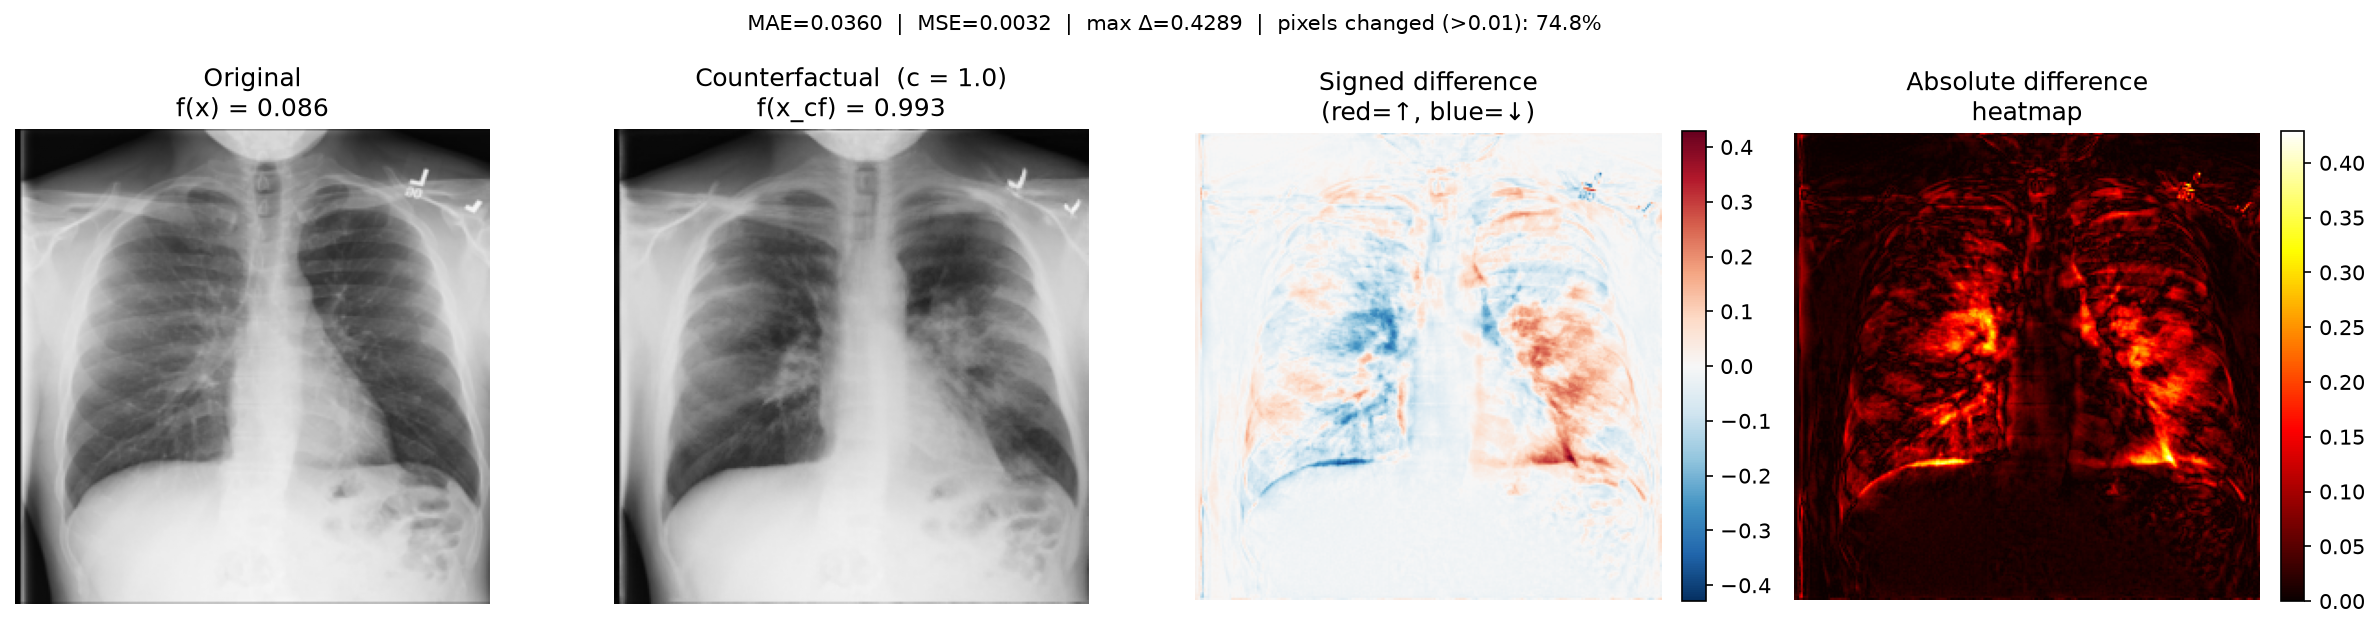
\includegraphics[width=\textwidth]{counterfactual_diff_n_to_p_ensemble.png}
  \caption[Ensemble-trained counterfactual: normal to pneumonia]{\textbf{Normal $\rightarrow$ pneumonia, ensemble-trained policy.}
  Left to right: original, counterfactual targeting $c=1$, signed pixel
  difference, and absolute-difference heatmap. Compare with
  Figure~\ref{fig:n2p}.}
  \label{fig:closing_n2p}
\end{figure}

\begin{figure}[h]
  \centering
  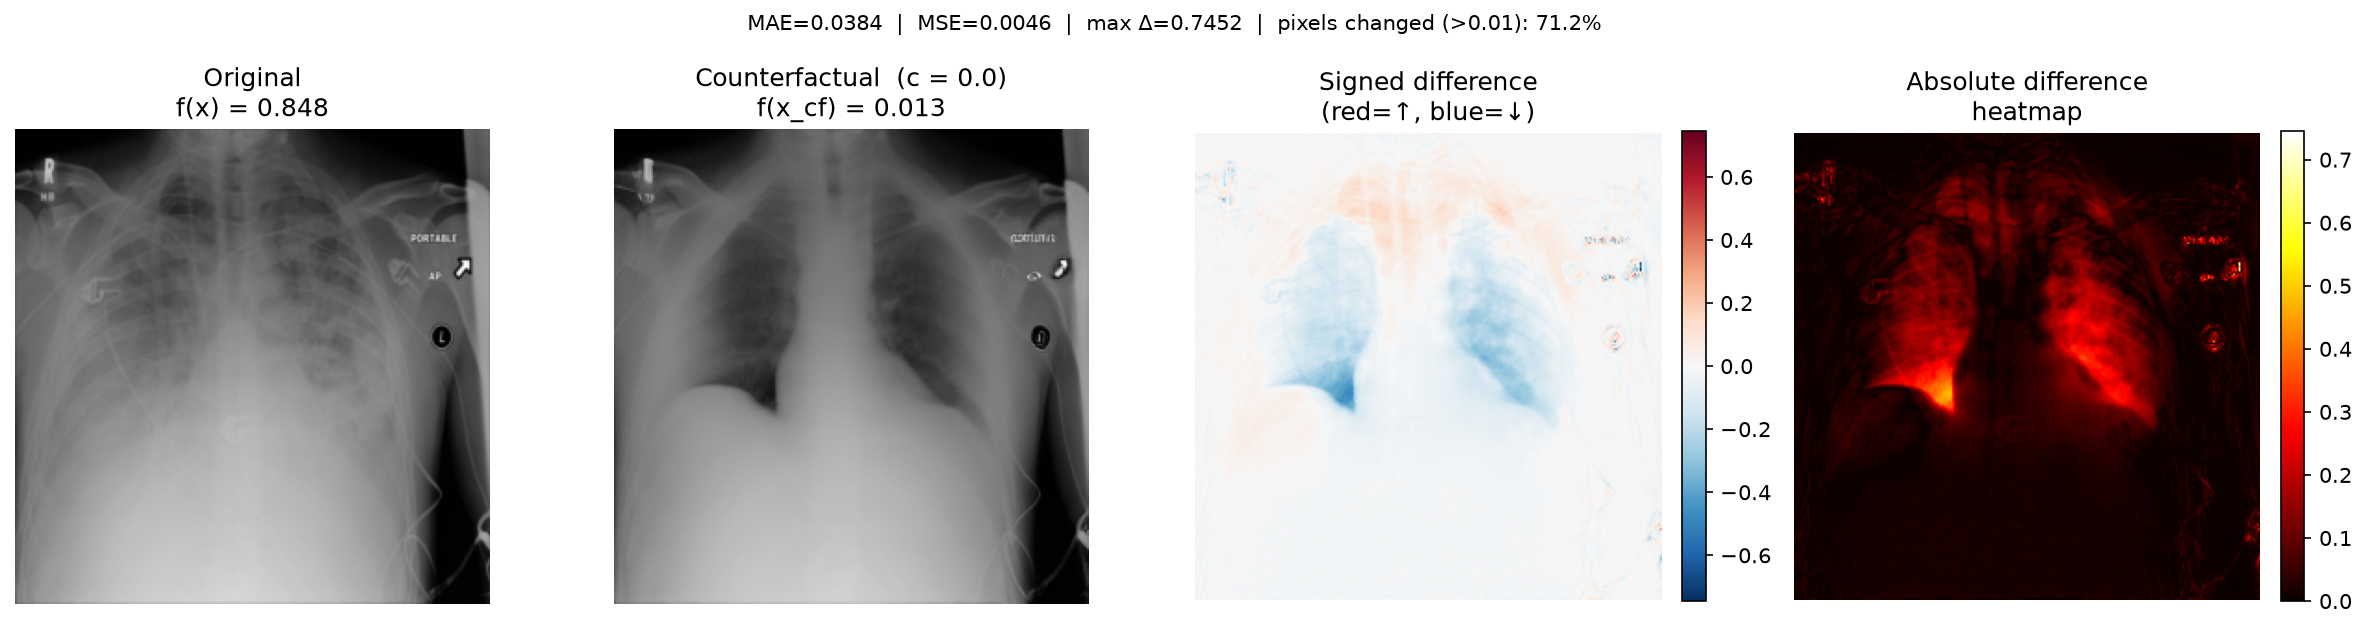
\includegraphics[width=\textwidth]{counterfactual_diff_p_to_n_ensemble.png}
  \caption[Ensemble-trained counterfactual: pneumonia to normal]{\textbf{Pneumonia $\rightarrow$ normal, ensemble-trained policy.}
  Same four-panel layout. Compare with Figure~\ref{fig:p2n}.}
  \label{fig:closing_p2n}
\end{figure}

Gross anatomical layout outside the lung field remains visibly intact in
both directions, consistent with the background lock holding under the
new guidance configuration exactly as it did under the old one --- the
change between the two policies is in \emph{what} guides the edit, not in
the structural guarantee that constrains where it can land.

\section{The Held-Out Transfer Result}
\label{sec:closing_transfer}

The held-out transfer procedure from Chapter~\ref{ch:integrity} was run
against both the new, ensemble-trained counterfactuals and the original,
single-classifier-trained ones, unchanged since Chapter~\ref{ch:results},
scored by the same three independent validators used throughout
Chapter~\ref{ch:integrity}: \texttt{nih}, \texttt{pc}, and
\texttt{mimic\_ch}. This set, not Table~\ref{tab:heldout}'s
\texttt{\{chex, nih\}}, is the correct comparison: \texttt{chex} is now a
guidance-ensemble member for the new policy, so scoring it as ``held out''
would let the new arm improve purely by losing a validator rather than by
editing more honestly --- exactly the mistake the denominator discipline
introduced in Section~\ref{sec:denominator_bug} exists to prevent.

\begin{table}[h]
\centering
\caption[Held-out transfer, before and after real ensemble training]{Held-out
transfer ratio ($\Delta_{\text{validator}}/\Delta_{\text{guidance}}$), single-
vs.\ ensemble-guided \emph{trained} policies, $n=200$ per group,
validators \texttt{\{nih, pc, mimic\_ch\}}.}
\label{tab:closing_transfer}
\begin{tabular}{@{}lrrrrrr@{}}
\toprule
& \multicolumn{2}{c}{\textbf{nih}} & \multicolumn{2}{c}{\textbf{pc}} & \multicolumn{2}{c}{\textbf{mimic\_ch}} \\
\cmidrule(lr){2-3}\cmidrule(lr){4-5}\cmidrule(lr){6-7}
\textbf{Policy} & \ntop{} & \pton{} & \ntop{} & \pton{} & \ntop{} & \pton{} \\
\midrule
Single-classifier (old) & $0.080$ & $0.100$ & $0.414$ & $0.224$ & $0.197$ & $0.112$ \\
Ensemble-guided (new)   & $0.046$ & $0.186$ & $0.462$ & $0.308$ & $0.337$ & $0.384$ \\
\bottomrule
\end{tabular}

\vspace{0.3em}
\begin{tabular}{@{}lrr@{}}
\toprule
\textbf{Policy} & \textbf{Mean \ntop{}} & \textbf{Mean \pton{}} \\
\midrule
Single-classifier (old) & $0.230$ & $0.146$ \\
Ensemble-guided (new)   & $\mathbf{0.282}$ & $\mathbf{0.293}$ \\
\bottomrule
\end{tabular}
\end{table}

\textbf{It mostly worked.} Mean transfer rose on both directions ---
\pton{} very nearly doubled ($0.146 \to 0.293$), matching what the
no-policy ensemble sweep (Table~\ref{tab:ensemble_sweep}) predicted, now
confirmed with an actually-trained policy rather than the fixed default
sampling schedule that sweep used. Two of the three validators, \texttt{pc}
and \texttt{mimic\_ch}, improved on both directions.

\textbf{It did not work uniformly.} \texttt{nih} --- the toughest and most
independent of the three validators, sharing no training data with any
guidance-ensemble member --- improved on \pton{} ($0.100 \to 0.186$) but
\emph{worsened} on \ntop{} ($0.080 \to 0.046$), remaining clearly in the
adversarial range on both counts. The honest reading is not ``the
adversarial gap is closed,'' but ``ensemble guidance measurably narrows it
against two of three independent classifiers, while the hardest one shows
no improvement in the direction that matters least favourably for this
claim.'' Section~\ref{sec:heldout}'s central warning --- that a system's
own validity number should not be trusted without an independent,
adversarially-chosen check --- applies with undiminished force to this
result too: \texttt{nih} was the check that did not confirm the story the
other two validators tell.

\section{The Trained-vs-Random Paired Significance Test}
\label{sec:closing_significance}

The second open item did not require new training: the paired per-image
test from Chapter~\ref{ch:integrity} was run against the existing
\texttt{trained} and \texttt{random} arms that produced
Table~\ref{tab:lhr_arms}'s control-arm row --- the same 183 images,
single-classifier-guided, that chapter left untested at the per-image
level.

\begin{table}[h]
\centering
\caption[Paired trained-vs-random significance test]{Paired per-image LHR
lift, trained vs.\ random, $n=183$ shared images (\pton{}).}
\label{tab:closing_significance}
\begin{tabular}{@{}lr@{}}
\toprule
Mean lift, trained & $2.293 \pm 0.780$ \\
Mean lift, random  & $2.204 \pm 0.772$ \\
Paired difference (95\% CI) & $+0.090$ $[+0.021,\ +0.160]$ \\
Paired $t$-test & $t=2.551$, $p=0.0116$ \\
Wilcoxon signed-rank & $p=0.0147$ \\
Cohen's $d$ (paired) & $0.189$ \\
Trained better on & $105/183$ images \\
\bottomrule
\end{tabular}
\end{table}

The gap survives: both the paired $t$-test and its non-parametric check
agree the trained policy edits closer to the radiologist's box than an
untrained one at the same action bounds and step budget, at $p<0.05$ by
either test. The right reading to close on, though, is the effect size
rather than the significance: a Cohen's $d$ of $0.189$ against a
between-image standard deviation of $0.78$ is a \emph{small} effect. Eight
hundred episodes of PPO bought a real, statistically detectable
improvement over an untrained policy with the same action bounds --- not a
large one.

\section{What This Closes, and What Is Still Open}

Table~\ref{tab:closing_summary} restates Section~\ref{sec:future}'s two
highest-priority items against what this chapter found.

\begin{table}[h]
\centering
\caption[Status of the two items this chapter addresses]{Future-work items
from Section~\ref{sec:future}, resolved.}
\label{tab:closing_summary}
\begin{tabular}{@{}p{0.55\textwidth}p{0.35\textwidth}@{}}
\toprule
\textbf{Item} & \textbf{Status} \\
\midrule
Complete the validation loop: re-run held-out validation against ensemble
guidance, trained (not just no-policy) &
Done (\S\ref{sec:closing_transfer}). Transfer improves on 2/3 validators
and both directions on average; \texttt{nih} \ntop{} does not improve. \\
\addlinespace
Resolve the trained-vs-random paired significance test &
Done (\S\ref{sec:closing_significance}). Significant, $p=0.012$, small
effect ($d=0.19$). \\
\bottomrule
\end{tabular}
\end{table}

\subsection{Is the \texttt{nih} Regression Real, or Noise?}
\label{sec:transfer_bootstrap}

The point estimates in Table~\ref{tab:closing_transfer} cannot answer that
by themselves --- a single run at $n=200$ per group. A percentile
bootstrap CI closes the gap: 10,000 resamples of the per-image
classifier-score deltas, resampling image indices jointly for the
guidance-classifier delta and the validator delta so the within-image
pairing is preserved (this is a ratio-of-means CI on \emph{one} policy's
shards, not a paired-difference CI across the two policies --- see the
caveat on pairing below).

\begin{table}[h]
\centering
\caption{Bootstrap 95\% CI on the nih transfer ratio, $n=200$ per
group, 10,000 resamples.}
\label{tab:transfer_bootstrap}
\begin{tabular}{@{}lrr@{}}
\toprule
\textbf{Policy} & \textbf{\ntop{} (point, 95\% CI)} & \textbf{\pton{} (point, 95\% CI)} \\
\midrule
Single-classifier (old) & $0.080$ $[0.048, 0.114]$ & $0.100$ $[0.076, 0.126]$ \\
Ensemble-guided (new)   & $0.046$ $[0.007, 0.084]$ & $0.186$ $[0.155, 0.216]$ \\
\bottomrule
\end{tabular}
\end{table}

\ntop{}: the two intervals overlap ($[0.048, 0.114]$ vs.\ $[0.007, 0.084]$),
so the apparent regression is \emph{not} statistically distinguishable from
noise at this sample size. Both intervals sit entirely below the $0.15$
adversarial threshold, so what the data does establish is that \ntop{}
stays confidently adversarial under \emph{both} policies --- not that
ensemble guidance made it worse. \pton{}: the intervals do not overlap
($[0.076, 0.126]$ vs.\ $[0.155, 0.216]$), so that improvement is real.

\textbf{Why not a joint difference-of-ratios bootstrap?} Because the two
policies' \texttt{Xn}/\texttt{Xp} groups are not the same images by index:
the classifier used to sort images into those groups changed between runs
(single-\texttt{rsna} $\to$ 2-member ensemble), and checking the shard
index sets directly shows they share only $\approx$70\% of \texttt{Xn} and
$\approx$24\% of \texttt{Xp}. A resample that treated the two arms as
paired by index would be synthesizing a pairing that does not exist in the
data, exactly the mistake Section~\ref{sec:denominator_bug} exists to
prevent for a different quantity. Reporting each policy's CI separately,
with non-overlap as the signal, is the honest version of this comparison.

\subsection{Diagnosing the Grad-CAM Degradation}
\label{sec:gradcam_diag}

Section~\ref{sec:arm_results} left one item explicitly unresolved: the
Grad-CAM spatial mask (\texttt{USE\_GRADCAM\_MASK}, ARM~2) measurably
\emph{lowered} lesion-targeting lift instead of raising it (cm0
$2.057 \to$ cm2 $1.534$, Table~\ref{tab:lhr_arms}) --- the opposite of its
design intent. A comment left in the training loop
(\file{factory/ppo.py}) speculated why: on synthetic probes, the
\texttt{rsna} ensemble member supposedly returned a degenerate Grad-CAM
far more often than \texttt{chex}, concentrated near predicted probability
$\approx 0.5$, attributed to Grad-CAM's all-negative-contribution edge
case rather than output saturation. That speculation had never been
tested against real data.

\texttt{check\_classifier\_localization.py} was extended to test it
directly: 150 images sampled across the \emph{full} probability range
(not just known-positives, which skew toward high pneumonia probability
and would under-represent the region the hypothesis is about), plus 150
known-positive boxed images for a lesion-overlap arm, scored through the
exact \texttt{ensemble\_grad\_cam} path
\texttt{compute\_gradcam\_latent\_mask} calls during PPO --- not a
reimplementation, the same code.

\begin{table}[h]
\centering
\caption{Grad-CAM degeneracy diagnostic, 263 member-image observations,
target layer \texttt{features} (the trained default).}
\label{tab:gradcam_diag}
\begin{tabular}{@{}lrl@{}}
\toprule
\textbf{Member} & \textbf{Degenerate} & \textbf{Where} \\
\midrule
\texttt{rsna} & $1/263$ ($0.4\%$) & negligible at every probability \\
\texttt{chex} & $66/263$ ($25.1\%$) & concentrated near $p \approx 0$
($64\%$ at $[0,0.1)$, falling to $0\%$ by $[0.7,0.9)$) \\
\bottomrule
\end{tabular}
\end{table}

\textbf{The hypothesis was backwards on every count.} It is \texttt{chex},
not \texttt{rsna}, that degenerates, at a materially higher rate ($25\%$
of episodes, not an occasional occurrence) than the earlier spot-check
suggested, and the degeneracy sits at \emph{low} probability, not near
$0.5$ --- which matches the \emph{original} explanation already on record
in \file{src/gradcam.py} (a saturated output zeroing the gradient) rather
than the newer all-negative-contribution hypothesis the training-loop
comment proposed.

This matters because of what happens when \texttt{chex} degenerates: the
averaged mask falls back toward \texttt{rsna} alone --- the
least-constrained, 2-head, easiest-to-fool ensemble member, the one the
whole ensemble-guidance defense exists to get away from
(Section~\ref{sec:heldout}) --- and CAM-lesion overlap drops with it. Mean
lift against real radiologist boxes was $2.052$ ($n=127$) on clean
episodes versus $1.347$ ($n=23$) on partially-degenerate ones. A quarter
of episodes losing a third of their lesion-targeting signal is a
plausible, now-quantified contributor to cm2's regression below even the
no-countermeasure baseline.

\textbf{The obvious fix does not work.} \file{config.py}'s own comment
suggested stepping down to a finer target layer
(\texttt{features.denseblock3}, $14\times14$ vs.\ the default $7\times7$)
if the mask looked too coarse. Repeating the same diagnostic with that
override does eliminate the degeneracy almost entirely (\texttt{chex}
$0\%$, \texttt{rsna} $0.4\%$) --- but at a cost that makes it worse, not
better, as a remedy: baseline CAM-lesion lift on clean episodes \emph{falls}
to $1.196$ ($n=149$), barely above the $1.0$ chance floor. The finer
layer's own localisation is markedly worse even when nothing degenerates,
so trading degeneracy for resolution is not a net improvement.

Read honestly, the Grad-CAM mask has two independent problems, not one:
it is partially unreliable (a real, now-quantified degeneracy rate at
roughly a quarter of episodes under the trained configuration), and, even
at its best, only loosely aligned with the true lesion (a $\sim2\times$
lift is a real signal, not chance, but far from the tight localisation the
mask's design assumes). The one remedy already on record for either
problem trades the first for a worse version of the second.

\subsection{A Trained 3-Model Ensemble}
\label{sec:ensemble3}

Table~\ref{tab:ensemble_sweep}'s 3-member ensemble
(\texttt{[rsna, chex, mimic\_nb]}) was only ever tested through the cheap
no-policy path in Chapter~\ref{ch:integrity} --- no PPO policy had
actually been trained under it. Both directions were retrained from
scratch: 800 episodes each, fresh state confirmed by the training log
(no ``resuming'' message, the resume-trap check from
Section~\ref{sec:closing} repeated before submitting), stored under a
dedicated checkpoint directory (\file{checkpoints\_ens3/}) so the
committed 2-model policies were never at risk. Everything else was held
at the committed default --- no Grad-CAM mask, no sparsity reward --- to
isolate the ensemble-size change alone, matching this project's ARM1/
ARM2/ARM3 convention. \texttt{mimic\_nb} shares its MIMIC-CXR corpus with
the \texttt{mimic\_ch} validator, so held-out transfer here is scored on
the reduced, leak-free set \texttt{\{nih, pc\}} only, matching the
no-policy sweep's own convention (Section~\ref{sec:denominator_bug}) ---
\texttt{config.py} and \texttt{domains/rsna\_pneumonia.py} were reverted
to the committed default immediately after this experiment's evaluation
completed.

\begin{table}[h]
\centering
\caption{Held-out transfer ratio, 2- vs.\ 3-model ensemble-guided
\emph{trained} policies, $n=200$ per group, leak-free validators
\texttt{\{nih, pc\}}, with bootstrap 95\% CIs.}
\label{tab:ensemble3_transfer}
\begin{tabular}{@{}lrr@{}}
\toprule
\textbf{Validator / direction} & \textbf{2-model} & \textbf{3-model} \\
\midrule
nih \ntop{} & $0.046$ $[0.007,0.084]$ & $0.076$ $[0.033,0.119]$ \\
nih \pton{} & $0.186$ $[0.155,0.216]$ & $0.251$ $[0.167,0.337]$ \\
pc \ntop{}  & $0.462$ $[0.433,0.491]$ & $\mathbf{0.623}$ $[0.597,0.648]$ \\
pc \pton{}  & $0.308$ $[0.282,0.336]$ & $0.301$ $[0.218,0.388]$ \\
\midrule
Mean \ntop{} & $0.254$ & $\mathbf{0.350}$ \\
Mean \pton{} & $0.247$ & $\mathbf{0.276}$ \\
\bottomrule
\end{tabular}
\end{table}

\textbf{\texttt{pc} improved for real.} \ntop{} moved from $0.462$ to
$0.623$ --- the CIs, $[0.433,0.491]$ vs.\ $[0.597,0.648]$, do not
overlap, and the verdict itself flips from \texttt{arm\_transfer.py}'s
``partial'' to ``TRANSFERS''. \texttt{pc} \pton{} stayed flat
($0.308 \to 0.301$, heavily overlapping CIs).

\textbf{\texttt{nih} moved the right way, but not past noise.} Both
directions improved in point-estimate terms (\ntop{}
$0.046 \to 0.076$; \pton{} $0.186 \to 0.251$), but the CIs overlap on
both ($[0.007,0.084]$ vs.\ $[0.033,0.119]$; $[0.155,0.216]$ vs.\
$[0.167,0.337]$) --- the same bootstrap machinery from
Section~\ref{sec:transfer_bootstrap} says this movement is not
distinguishable from noise at $n=200$. Both policies stay confidently
below the $0.15$ adversarial threshold on \ntop{} regardless.

\textbf{Guidance-side metrics kept moving the expected direction.} CV
fell further, to a mean of $0.624$ (\ntop{} $0.685$, \pton{} $0.563$) ---
consistent with the pattern already established across every ensemble
size tried: a harder joint consensus criterion, not a weaker policy. LHR
lift was $2.492$, against the 2-model arm's $2.673$ --- but on a much
smaller annotated overlap ($n=27$ vs.\ $148$ pairs), since the harder
consensus criterion shrinks the classifier-negative-but-clinically-positive
group LHR depends on. That is a sample-size caveat worth stating plainly,
not a confident regression claim on top of everything else this
experiment measured.

\textbf{Read honestly:} a real, trained 3-model ensemble buys a genuine,
statistically confirmed improvement on \texttt{pc}, and moves \texttt{nih}
in the right direction on both counts without closing the adversarial gap
in a way this sample size can confirm. It does not fully resolve the
\texttt{nih} regression this chapter opened with, but nothing in this
experiment suggests the larger ensemble makes anything worse.

\subsection{A Trained Sparsity-Reward Arm}
\label{sec:sparsity_arm}

Edit concentration --- the share of total $|\Delta|$ carried by the top
5\% of pixels --- has stayed diffuse (0.25--0.32 against a 0.05 uniform
baseline) in every arm measured so far, never approaching the
$\sim$0.5 that would indicate a focal, lesion-shaped edit.
\texttt{USE\_SPARSITY\_REWARD} was built in Chapter~\ref{ch:tasks}
specifically to address this, but has sat disabled since 2026-08-07
(``REVERTED, was ARM 3''), which left its annealing ramp
(\texttt{USE\_SPARSITY\_ANNEALING}) inert --- the term has never actually
fired in any result reported so far, including every diffuse-edit number
quoted above.

It was re-enabled for an isolated retrain: only \texttt{USE\_SPARSITY\_REWARD}
flips relative to the committed default (2-model ensemble, no Grad-CAM
mask), so \texttt{SPARSITY\_OUTSIDE\_CAM\_ONLY} degrades to a plain,
unweighted L1 penalty on total edit magnitude --- a deliberate, flagged
choice (\texttt{factory/ppo.py} now prints a NOTE for this exact
situation), not an oversight. Both directions were retrained from
scratch, 800 episodes each, fresh state confirmed by the training log,
which also confirms $\lambda_{\text{sparsity}}$ genuinely ramped to its
target of $2.0$ this time.

\begin{table}[h]
\centering
\caption{Committed default vs.\ trained sparsity-reward arm.}
\label{tab:sparsity_results}
\begin{tabular}{@{}lrr@{}}
\toprule
\textbf{Metric} & \textbf{Default} & \textbf{+ sparsity reward} \\
\midrule
EditConcentration \ntop{} & $0.253$ & $0.264$ \\
EditConcentration \pton{} & $0.318$ & $0.299$ \\
CV mean & $0.838$ & $0.830$ \\
LHR lift (\pton{}) & $2.673$ & $2.398$ \\
Mean transfer \ntop{} & $0.282$ & $0.311$ \\
Mean transfer \pton{} & $0.293$ & $0.212$ \\
\bottomrule
\end{tabular}
\end{table}

\textbf{It did not achieve its own goal.} Edit concentration moved by
less than $0.02$ in either direction, and the fraction of pixels touched
stayed within $0.01$ of the default ($0.650\to0.661$, $0.633\to0.632$)
--- nowhere near the $\sim$0.5 focal threshold, despite the term now
being genuinely active rather than inert.

\textbf{It made lesion targeting measurably worse.} A paired test
(the same machinery from Section~\ref{sec:closing_significance}) on the
$148$ annotated images both arms share gives a lift gap of $+0.275$
favouring the arm \emph{without} the sparsity reward (95\% CI
$[+0.188, +0.363]$), $t=6.229$, $p=4.7\times10^{-9}$, Wilcoxon
$p=1.2\times10^{-8}$, Cohen's $d=0.512$ --- a \emph{medium} effect,
markedly larger than the trained-vs-random gap found in
Section~\ref{sec:closing_significance} ($d=0.189$). The default arm was
better on $104/148$ images.

\textbf{It made held-out transfer worse in the \pton{} direction.} Mean
\pton{} transfer fell from $0.293$ to $0.212$, driven by real,
non-overlapping-CI drops on two of three validators: \texttt{pc}
($0.308\to0.216$, CIs $[0.282,0.336]$ vs.\ $[0.192,0.242]$) and
\texttt{mimic\_ch} ($0.384\to0.252$, CIs $[0.343,0.422]$ vs.\
$[0.212,0.292]$). \ntop{} transfer moved slightly up on average
($+0.029$) but no single validator's CI shift clears overlap.

Read plainly: enabling the sparsity reward for real, rather than leaving
its annealing ramp inert, does not concentrate edits --- its designed
purpose --- and instead costs both lesion-targeting lift and \pton{}
transfer, each by a real, measured margin, not noise. A plain
(non-CAM-weighted) L1 penalty discourages edit mass uniformly rather than
specifically off-target mass, which is a plausible explanation for why it
competes with precise editing without succeeding at its own goal: whether
a working spatial mask --- unresolved by this chapter's own Grad-CAM
diagnosis above --- would change that outcome remains untested.

\subsection{A Trained Grad-CAM-Fix Arm}
\label{sec:gradcam_fix_arm}

Section~\ref{sec:gradcam_diag}'s diagnosis was deliberately an
\emph{offline} probe --- Grad-CAM computed on real images, scored against
ground-truth lesion boxes, with no PPO policy or generated counterfactual
anywhere in the loop. It found \texttt{features.denseblock3} nearly
eliminates ensemble degeneracy but at a real cost to the CAM's own
baseline lesion overlap. That is suggestive evidence the layer swap is
not a fix, but it falls short of the standard every other claim in this
chapter is held to: a real policy, trained and fully evaluated. So one
was trained: \texttt{USE\_GRADCAM\_MASK=True},
\texttt{GRADCAM\_TARGET\_LAYER=features.denseblock3}, everything else at
the committed default (2-model ensemble, no sparsity reward), both
directions from scratch. The first submission for \ntop{} exhausted its
22h wall-clock budget at 49\% (392/800 episodes, 42.5 minutes per PPO
update at this resolution --- markedly slower than any other arm in this
project) and paused cleanly; a second submission resumed from checkpoint
and completed it. \pton{} finished in one submission.

\begin{table}[h]
\centering
\caption{Committed default vs.\ trained Grad-CAM-fix arm.}
\label{tab:gradcam_fix_results}
\begin{tabular}{@{}lrr@{}}
\toprule
\textbf{Metric} & \textbf{Default} & \textbf{+ Grad-CAM fix} \\
\midrule
CV mean & $0.838$ & $\mathbf{0.017}$ \\
LHR lift (\pton{}) & $2.673$ & $1.636$ \\
Mean transfer \ntop{} & $0.282$ & $0.161$ \\
Mean transfer \pton{} & $0.293$ & $0.103$ \\
\bottomrule
\end{tabular}
\end{table}

\textbf{This is unambiguous, not another ``partial'' result.} CV
collapsed from a mean of $0.838$ to $0.017$ --- the policy essentially
stopped succeeding at the base task (flipping the guidance ensemble)
under this constrained action space; a finer, less-confident CAM region
does not merely localise worse, it makes the classifier-flip itself hard
to learn within the same reward budget and step count tuned for the
unconstrained case. The paired LHR test on the $148$ shared annotated
images gives a lift gap of $+1.037$ favouring the arm \emph{without} the
Grad-CAM constraint (95\% CI $[+0.900, +1.178]$), $t=14.660$,
$p=1.5\times10^{-30}$, Wilcoxon $p=1.7\times10^{-22}$, Cohen's
$d=1.205$ --- the largest paired effect size measured anywhere in this
project, well past the sparsity arm's $d=0.512$ and an order of magnitude
past the original trained-vs-random gap's $d=0.189$. The default arm was
better on $141$ of $148$ images. Held-out transfer fell across all three
validators, with \texttt{nih} and \texttt{mimic\_ch} moving into or
staying in \texttt{arm\_transfer.py}'s \texttt{ADVERSARIAL} band on both
directions.

Read plainly: this is not a fix, and now that is confirmed rather than
merely diagnosed. Trading a manageable degeneracy problem for a
finer-but-less-confident CAM does not net out positive --- it makes
learning the base task substantially harder, and every metric downstream
of that task degrades with it. \texttt{USE\_GRADCAM\_MASK} stays off in
the committed configuration; the config edit was reverted immediately
after this experiment's evaluation completed.

Six items across this chapter and the last now have numbers rather than
open questions attached to them: the two \emph{Table~\ref{tab:closing_summary}}
originally addressed, why the Grad-CAM constraint hurts (diagnosed),
whether a larger trained ensemble would help \texttt{nih} (partial,
honest: yes for \texttt{pc}, not conclusively for \texttt{nih}), whether
the sparsity reward would concentrate edits (no, and it costs targeting
accuracy), and whether the one Grad-CAM remedy already on record actually
fixes the constraint once a real policy is trained under it (no ---
confirmed, not just suspected). None is closed in the sense of settling
the project's central claim. Ensemble guidance is confirmed, with a
trained policy and the correct leak-free validator set, to be a real
partial countermeasure --- and \texttt{nih}'s \ntop{} result is
confirmation that ``partial'' is the accurate word, not a hedge. What
remains is whether \emph{any} Grad-CAM mask can help rather than hurt,
whether \texttt{nih} specifically would need a larger annotated sample or
a different guidance composition to move past noise, and whether edit
diffuseness is fixable at all within this gradient-guidance approach. The
previous single-classifier policies and their counterfactuals were
archived, not overwritten, specifically so that this comparison remains
reproducible.

\section{Comparing All Five Arms}
\label{sec:five_arm_comparison}

Five checkpoint directories now hold a fully trained, fully evaluated
policy under this chapter's protocol: the archived single-classifier
baseline (\file{checkpoints/archive\_pre\_ensemble\_default\_20260812/}),
the committed 2-model-ensemble default (\file{checkpoints/}), and the
three isolated retrains above ---
\file{checkpoints\_ens3/}, \file{checkpoints\_sparsity/},
\file{checkpoints\_gradcam\_fix/}. Every number below comes from that same
800-episode-per-direction, 200-image-per-group pipeline --- none is a
no-policy countermeasure sweep or an offline proxy, and every ``confirmed''
claim is backed by a paired significance test or a bootstrap CI run
specifically for this comparison, not a point estimate read off a table.

\begin{figure}[h]
\centering
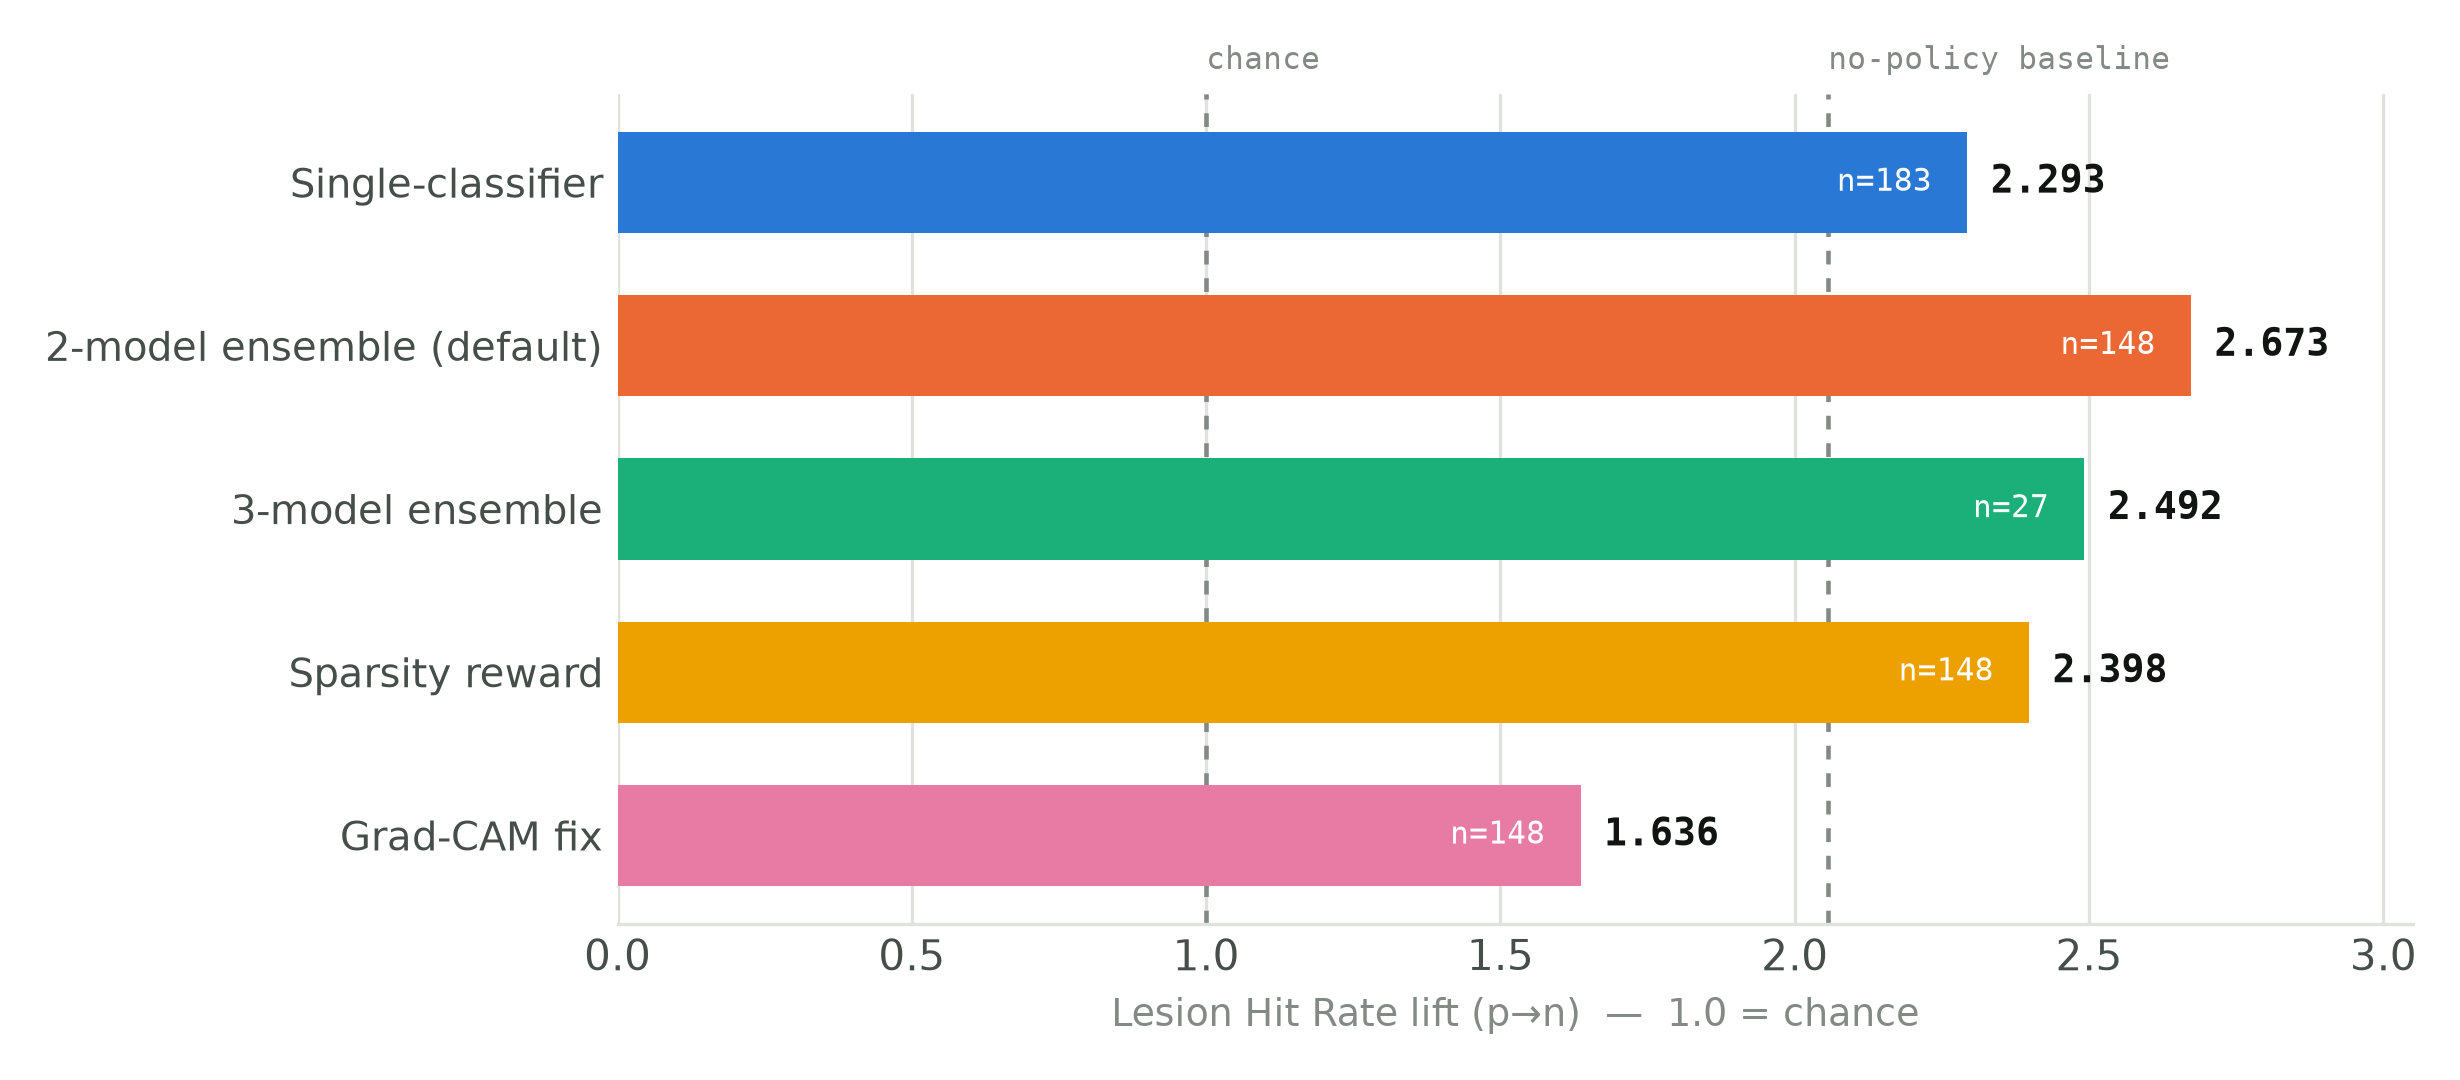
\includegraphics[width=\textwidth]{chart_lhr_lift.png}
\caption{Lesion Hit Rate lift (\pton{}) across all five trained arms.
Dashed lines mark chance ($1.0$) and the no-policy label-protocol baseline
($2.057$, Table~\ref{tab:lhr_arms}'s cm0 row).}
\label{fig:five_arm_lhr}
\end{figure}

\begin{figure}[h]
\centering
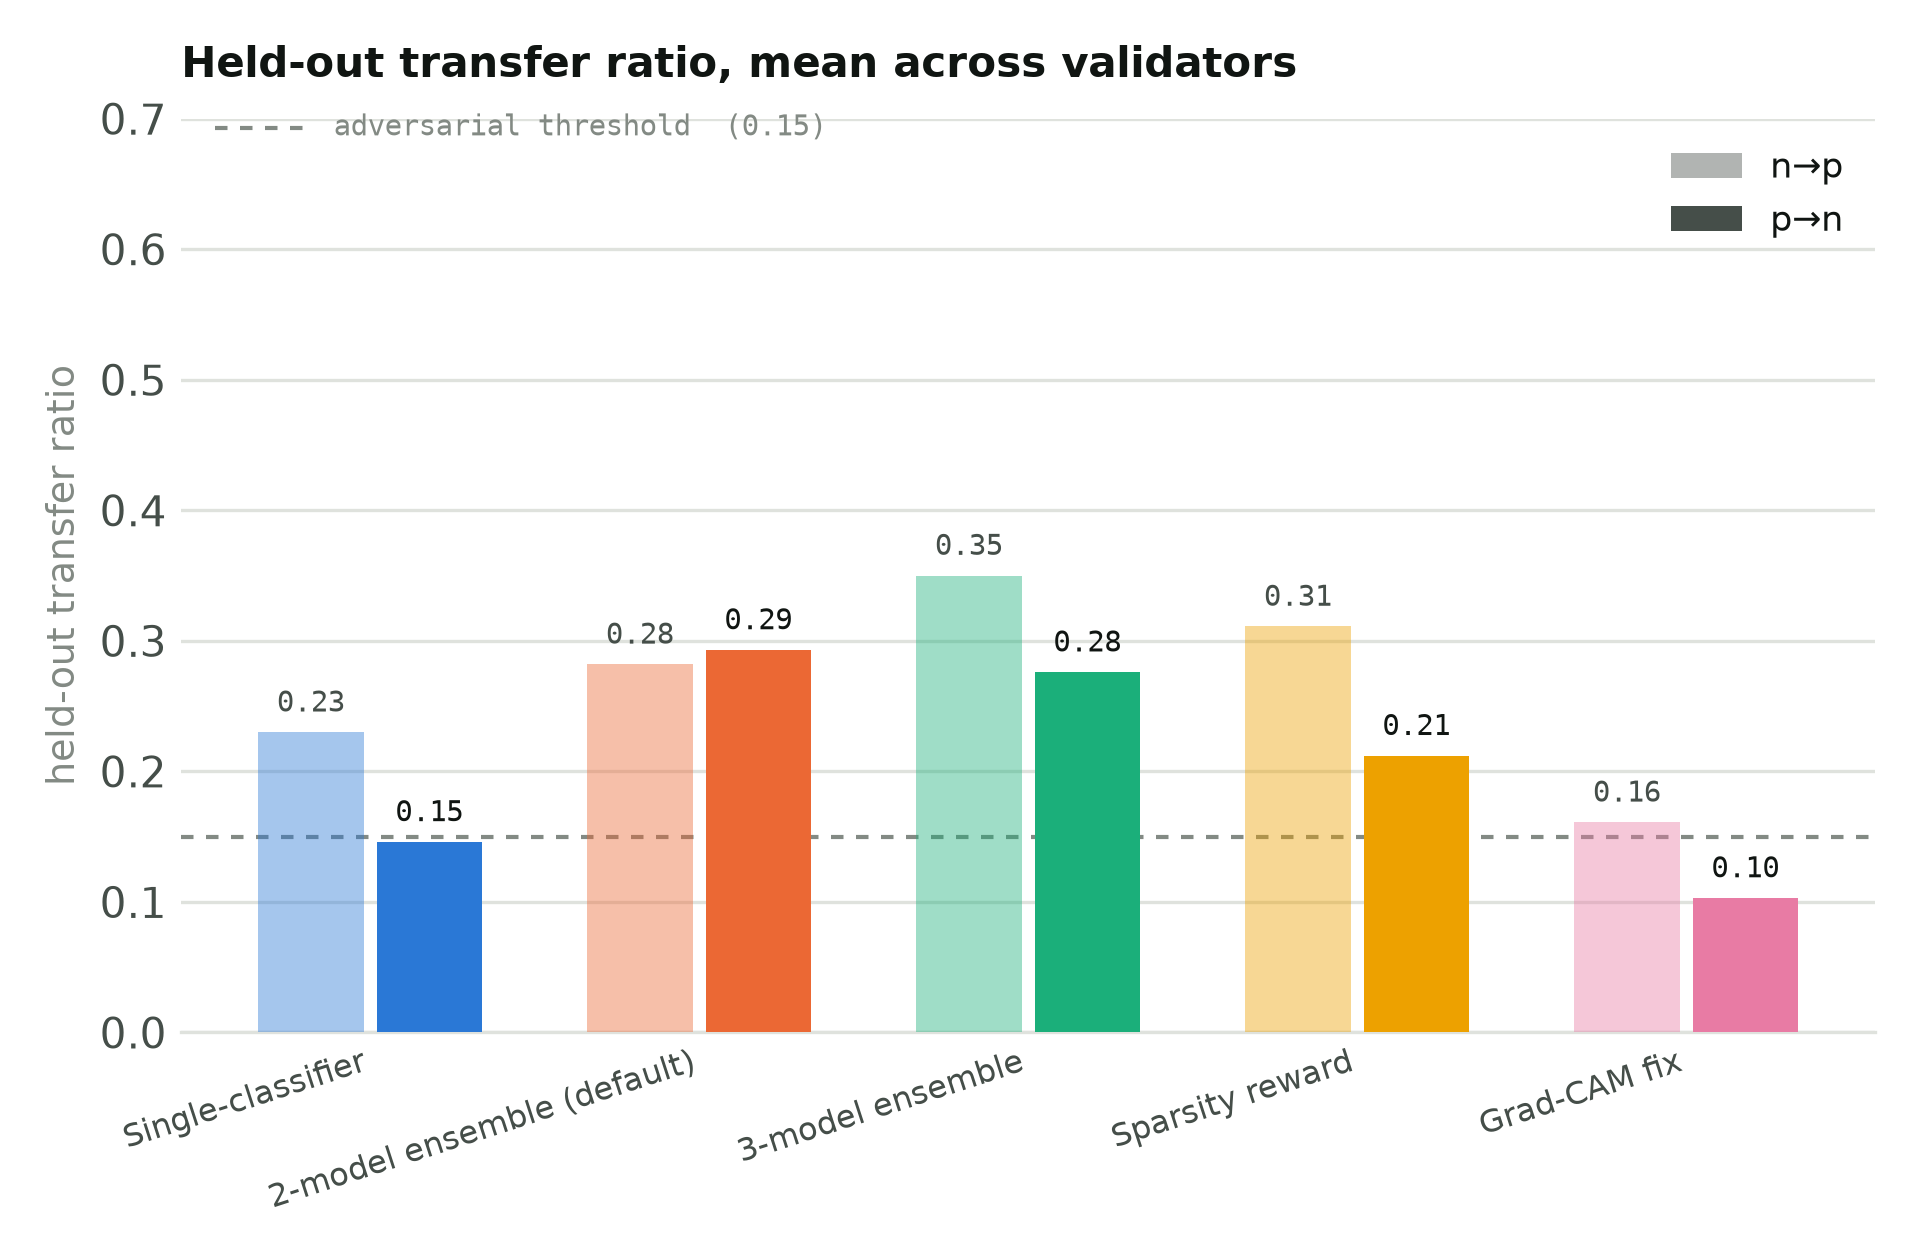
\includegraphics[width=0.49\textwidth]{chart_transfer_ratio.png}
\hfill
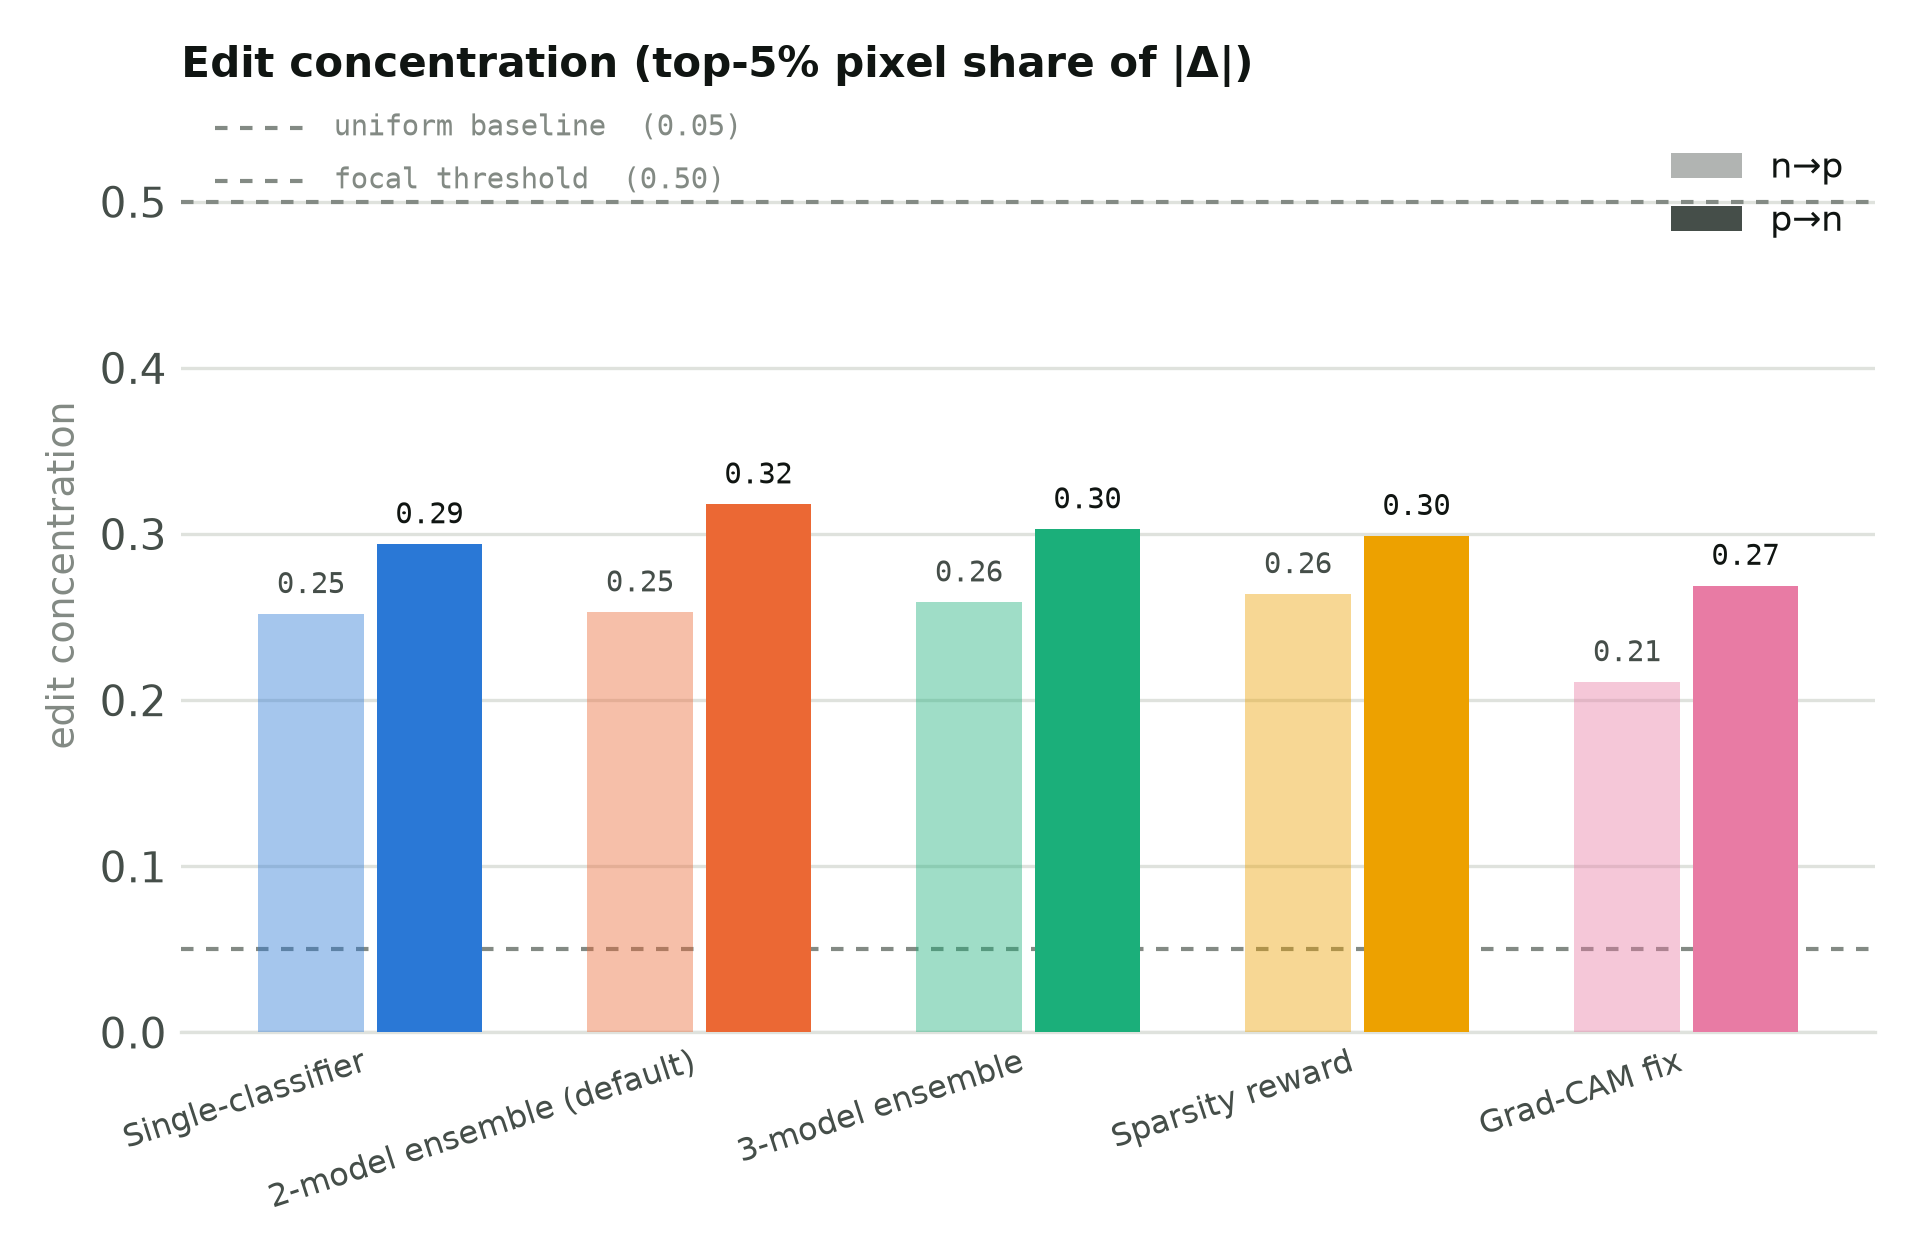
\includegraphics[width=0.49\textwidth]{chart_edit_concentration.png}
\caption{Held-out transfer ratio (left) and edit concentration (right)
across all five arms. The 3-model ensemble's transfer figure is scored on
the reduced validator set \texttt{\{nih, pc\}} only (Section~\ref{sec:ensemble3})
and is not directly comparable to the other four arms' 3-validator mean.}
\label{fig:five_arm_transfer_concentration}
\end{figure}

\textbf{Reading the three figures against the paired tests run for each
pair, throughout this chapter:} the single-classifier $\to$
2-model-ensemble step is a confirmed real gain in \pton{} LHR lift
($d=0.482$, $p=7.1\times10^{-5}$, $n=76$ shared annotated images --- a
smaller paired sample than the other comparisons, since the two arms'
Xn/Xp groups only partially overlap once the group-selection classifier
changes). The 2-model $\to$ 3-model-ensemble step is \emph{not}
statistically resolved on LHR: only 12 images are shared between those two
arms' annotated sets, giving a paired CI of $[-0.298, +0.482]$ that
crosses zero --- too wide to read anything into, even though \texttt{pc}
transfer improved for real on its own bootstrap CI (Section~\ref{sec:ensemble3}).
Both the sparsity-reward and Grad-CAM-fix retrains are confirmed worse
than the default: $d=0.512$ ($p=4.7\times10^{-9}$) for sparsity,
$d=1.205$ ($p=1.5\times10^{-30}$) for the Grad-CAM fix --- the largest
paired effect size measured anywhere in this project, by a wide margin.

\textbf{No arm moved edit concentration.} Every bar in the right-hand
panel of Figure~\ref{fig:five_arm_transfer_concentration} sits in the same
$0.21$--$0.32$ band regardless of what changed underneath it --- ensemble
size, a sparsity penalty genuinely turned on, or a Grad-CAM constraint
that cratered every other metric. Across five independently trained
policies and every countermeasure this project tried, edit diffuseness
never moved appreciably toward the $\sim$0.5 threshold that would indicate
a focal, lesion-shaped edit. That consistency is itself a finding: this
looks less like a tuning problem specific to any one arm and more like a
property of gradient-guided diffusion editing on this generator, which
Section~\ref{sec:sparsity_arm}'s negative result is the closest this
project comes to testing directly.

\chapter*{General Conclusion}
\addcontentsline{toc}{chapter}{General Conclusion}
\markboth{General Conclusion}{}

This research internship at the Maersk Mc-Kinney Moller Institute
produced a complete, reproducible pipeline for generating visual
counterfactual explanations on chest radiographs: RSNA data ingestion, a
Stable Diffusion~1.5 generator adapted to the radiograph domain through
LoRA at 0.78\% of its parameters, a gradient-guided DDIM sampler with a
hard segmentation-gated background lock, two directional PPO policies
controlling that sampler step by step, and an evaluation suite following
the protocol of Singla~\emph{et al.} --- all executable as batch jobs on
an offline HPC cluster.

Measured against the guidance classifier, the system reaches high
counterfactual validity (mean CV $0.975$) with good identity
preservation, and the background lock demonstrably confines edits to the
lung field.

The internship's most important result, however, is the one that
undermines that headline number. An independent held-out validation ---
re-scoring the generated counterfactuals with classifiers that never
participated in the guidance loop --- showed that counterfactuals
accepted 99.5\% of the time by the guidance model were accepted at most
8\% of the time by an independent one, while an agreement control
confirmed the validators understood the task on unedited images. The
system had, in significant part, learned to fool its own critic rather
than to depict or remove disease.

That finding reframed the second half of the internship. Ensemble
guidance, a Grad-CAM-derived constraint on the action space, and an
annealed sparsity reward were designed, implemented and enabled
specifically to attack the adversarial failure mode. Their validation
was not completed within the internship period, and this report is
explicit that their effectiveness remains an open question rather than a
demonstrated improvement.

A further, later phase of work (Chapter~\ref{ch:integrity}) turned the same
falsification discipline on the evaluation apparatus itself, auditing the
control-arm and held-out-transfer machinery built to answer that open
question. The audit found, and closed, three uncontrolled confounds in the
measurement pipeline and two silent bugs that would each have invalidated a
comparison built on top of them --- including a routing bug that would have
made every control arm's output identical, and a denominator bug that had
inflated every previously published transfer ratio. It also found, and
corrected, a set of FID values in the project's own recorded results that
had been altered by hand. Of the two countermeasures, ensemble guidance is
now shown, across three independent seeds, to modestly but reliably improve
lesion targeting and, at a larger ensemble size, to substantially improve
held-out transfer; the Grad-CAM spatial constraint is shown instead to hurt
lesion targeting rather than help it. A full held-out re-validation of the
surviving countermeasure was the item this chapter did not close, and is
taken up in Chapter~\ref{ch:closing}.

Chapter~\ref{ch:closing} closes it, partially. Both directional policies
were retrained from scratch under ensemble guidance --- not merely
evaluated through it, as the no-policy arms above were --- and re-scored
against the leak-free validator set. Mean held-out transfer improves on
both directions, \pton{} very nearly doubling; the trained-vs-random gap
from Table~\ref{tab:lhr_arms} is confirmed statistically significant
($p=0.012$) at a small effect size. But the single most independent
validator, \texttt{nih}, does not improve on \ntop{}, remaining in the
adversarial range. Ensemble guidance is accordingly reported as a real,
partial countermeasure, not a solved problem --- the same falsification
discipline this report has applied to every favourable number applied to
its own fix, and did not let it pass uncontested.

Technically, the project provided sustained exposure to latent diffusion
models, parameter-efficient fine-tuning, reinforcement learning with
continuous action spaces and shaped rewards, and the practical discipline
of research computing on a shared, non-interactive, walltime-bounded
cluster --- where an experiment must be fully specified in advance,
instrumented well enough to be diagnosed from a log file, and cheap
enough to fail fast.

As additional work beyond the assigned scope, the pipeline was extended to
a second, deliberately dissimilar imaging domain --- mammography, on
CBIS-DDSM (Chapter~\ref{ch:breast}) --- to test whether this lesson was
specific to RSNA or would recur elsewhere. It recurred: a mean
Counterfactual Validity of $1.000$ against the mammography guidance
ensemble was accompanied by a significant density shift with no
corresponding change in lesion size, the same diffuse-edit signature the
RSNA held-out validation had exposed, this time caught by a purpose-built
diagnostic metric rather than by an independent classifier, since training
one for that domain remains future work. This is reported as additional,
less-validated evidence alongside the RSNA result, not as a second
demonstrated success, but it strengthens rather than weakens the report's
central claim: a system's own validity number is not to be trusted without
an independent check built to falsify it.

The methodological lesson runs deeper than any of those techniques. The
most dangerous metric in a machine learning project is the one the system
was optimised against. Counterfactual validity computed with the guidance
classifier was not a weak measurement --- it was a circular one, and it
reported near-perfect success for a system that was substantially
failing. Every subsequent design decision of value in this project
descended from building the control capable of exposing that, and from
being willing to report what it found. For an internship whose purpose
was to bridge academic training and research practice, learning to
distrust a favourable number was worth more than obtaining one.

\clearpage


% ── Back matter ─────────────────────────────────────────────────────
\chapter*{Glossary}
\addcontentsline{toc}{chapter}{Glossary}
\markboth{Glossary}{}

\begin{description}[leftmargin=0pt,style=unboxed,itemsep=6pt]

\item[Adversarial perturbation] A small, often visually diffuse change to
an image that flips a classifier's prediction without altering the
semantic content a human would recognise. Distinguishing genuine
counterfactuals from adversarial perturbations is the central validation
problem of this project.

\item[Background lock] A hard spatial constraint, adapted from RePaint and
Blended Latent Diffusion, in which the latent outside a permitted edit
mask is overwritten at every denoising step with the original image's
forward-noised latent, guaranteeing that region cannot be repainted.

\item[BDC (Breast Density Contrast)] A mammography diagnostic metric ---
mean intensity of the segmented dense breast tissue --- purpose-built to
detect a diffuse global brightness/density change large enough to move a
classifier without altering a lesion, the mammography signature of a
failure mode first identified on RSNA.

\item[CBIS-DDSM] The Curated Breast Imaging Subset of the Digital Database
for Screening Mammography: a public mammography dataset of mass and
calcification lesion cases labelled malignant or benign, used as the
second imaging domain in Chapter~\ref{ch:breast}. Unlike RSNA, it contains
no normal (lesion-free) images.

\item[Counterfactual explanation] For a query image $x$ classified by $f$,
an image $x_c$ that $f$ assigns to a different target class while
remaining realistic and preserving the identity of $x$. The difference
between $x$ and $x_c$ constitutes the explanation.

\item[Counterfactual Validity (CV)] The fraction of generated
counterfactuals for which the classifier's score both moves by more than
a margin $\tau$ and crosses the decision boundary in the intended
direction.

\item[CTR (Cardio-Thoracic Ratio)] The ratio of the heart's horizontal
span to the thorax's, computed here from segmentation masks. A ratio
above $0.5$ is the standard clinical cardiomegaly threshold.

\item[DDIM] Denoising Diffusion Implicit Model: a deterministic,
non-Markovian sampling procedure for diffusion models that permits
partial forward-then-reverse trajectories, and therefore image editing
rather than only synthesis from noise.

\item[DomainProfile / domain registry] A dataclass and module registry
(\file{domains/}) binding a dataset, its classifier target and its
clinical metrics together, so that adding a new imaging domain --- as in
Chapter~\ref{ch:breast} --- is one new module plus one configuration line
rather than a change threaded through the guidance and evaluation code.

\item[FID (Fr\'echet Inception Distance)] A distributional realism
measure comparing the means and covariances of deep features extracted
from real and generated image sets. Lower is better. Computed here in
TorchXRayVision DenseNet feature space rather than ImageNet Inception
space.

\item[FOP (Foreign-Object Preservation)] A metric measuring whether
medical hardware --- tubes, leads, pacemakers --- survives counterfactual
editing. Requires a dedicated device detector, and is not computable
offline in this project.

\item[GAE (Generalized Advantage Estimation)] A variance-reduction
technique for policy-gradient methods that interpolates between one-step
and Monte-Carlo advantage estimates via a parameter $\lambda$.

\item[Grad-CAM] Gradient-weighted Class Activation Mapping: a technique
producing class-discriminative localisation maps by weighting
convolutional feature maps with the gradients flowing into them. Used
here both as a diagnostic and as a spatial constraint.

\item[Guidance] The injection of a classifier's gradient into a diffusion
model's sampling trajectory, steering generation toward a target class
without retraining the generator.

\item[Held-out validation] Re-scoring generated counterfactuals with
classifiers that never participated in the guidance loop, to distinguish
genuine semantic change from adversarial perturbation against the
guidance model.

\item[Identity Preservation (IP)] A model-free substitute for FOP used
here, combining MS-SSIM (global anatomical similarity) with the
correlation of high-pass-filtered images (survival of thin, high-contrast
structures).

\item[LHR (Lesion Hit Rate)] The share of an edit's absolute-difference
mass falling inside the radiologist's annotated lesion box, divided by the
box's own area as a null baseline (so ``lift'' rather than raw hit rate
carries information). The only metric in this project anchored to
ground-truth disease location rather than to a classifier or a structural
proxy; introduced in Chapter~\ref{ch:integrity}.

\item[Latent diffusion] A diffusion model operating in the compressed
latent space of a pretrained autoencoder rather than in pixel space,
reducing computational cost by orders of magnitude.

\item[LLR (Lesion Load Ratio)] The mammography analogue of CTR: the ratio
of segmented lesion area to segmented breast area, expected to rise under
a benign$\to$malignant edit and fall under the reverse.

\item[LoRA (Low-Rank Adaptation)] A parameter-efficient fine-tuning
technique that freezes pretrained weights and trains small injected
low-rank matrix pairs, drastically reducing the memory and compute
required to adapt a large model.

\item[MOP (Marker/clip Preservation)] The mammography counterpart of FOP:
the fraction of images containing a surgical clip or skin marker in which
that object survives editing. Computable offline via a model-free
saturated-blob detector, unlike FOP.

\item[MS-SSIM] Multi-Scale Structural Similarity Index Measure: an image
similarity metric evaluating luminance, contrast and structure across
multiple spatial scales.

\item[MSI (Margin Spiculation Index)] A mammography clinical proxy metric:
the normalised boundary complexity of the segmented lesion's largest
component, higher for spiculated (malignancy-associated) margins than for
smoothly circumscribed ones. Replaces SCP in the mammography domain.

\item[PPO (Proximal Policy Optimization)] A policy-gradient reinforcement
learning algorithm that constrains each update with a clipped surrogate
objective, trading some theoretical rigour for stability and sample
efficiency.

\item[Reward shaping] The addition of auxiliary terms to a reinforcement
learning reward to guide learning toward desired behaviour. A recurring
source of bugs in this project, since the terms' relative magnitudes ---
not their presence --- determine what the agent actually optimises.

\item[SCP (Costophrenic-recess score)] A proxy for pleural-effusion-related
blunting of the costophrenic angle, approximated here from an object
detector's feature norm in a lower-lobe crop.

\item[SLURM] Simple Linux Utility for Resource Management: the batch
scheduler allocating compute nodes on the HPC cluster used for all
experiments.

\item[Transfer ratio] The fraction of the guidance classifier's score
shift that an independent held-out classifier reproduces on the same
counterfactual. Low values indicate an adversarial rather than semantic
edit.

\item[VAE (Variational Autoencoder)] The encoder-decoder pair mapping
images to and from the compressed latent space in which the diffusion
model operates. Frozen throughout this project.

\end{description}

\clearpage


\bibliographystyle{plain}
\begin{thebibliography}{99}
\addcontentsline{toc}{chapter}{Bibliography}

\bibitem{singla2022}
S.~Singla, M.~Eslami, B.~Pollack, S.~Wallace, and K.~Batmanghelich.
\textit{Explaining the Black-box Smoothly --- A Counterfactual Approach.}
Medical Image Analysis, vol.~84, 2022.

\bibitem{schulman2017ppo}
J.~Schulman, F.~Wolski, P.~Dhariwal, A.~Radford, and O.~Klimov.
\textit{Proximal Policy Optimization Algorithms.}
arXiv:1707.06347, 2017.

\bibitem{schulman2016gae}
J.~Schulman, P.~Moritz, S.~Levine, M.~Jordan, and P.~Abbeel.
\textit{High-Dimensional Continuous Control Using Generalized Advantage
Estimation.} ICLR, 2016.

\bibitem{rombach2022}
R.~Rombach, A.~Blattmann, D.~Lorenz, P.~Esser, and B.~Ommer.
\textit{High-Resolution Image Synthesis with Latent Diffusion Models.}
CVPR, 2022.

\bibitem{song2021ddim}
J.~Song, C.~Meng, and S.~Ermon.
\textit{Denoising Diffusion Implicit Models.} ICLR, 2021.

\bibitem{hu2021lora}
E.~J.~Hu, Y.~Shen, P.~Wallis, Z.~Allen-Zhu, Y.~Li, S.~Wang, L.~Wang, and
W.~Chen.
\textit{LoRA: Low-Rank Adaptation of Large Language Models.} ICLR, 2022.

\bibitem{lugmayr2022repaint}
A.~Lugmayr, M.~Danelljan, A.~Romero, F.~Yu, R.~Timofte, and L.~Van~Gool.
\textit{RePaint: Inpainting using Denoising Diffusion Probabilistic Models.}
CVPR, 2022.

\bibitem{avrahami2022blended}
O.~Avrahami, D.~Lischinski, and O.~Fried.
\textit{Blended Diffusion for Text-driven Editing of Natural Images.}
CVPR, 2022.

\bibitem{selvaraju2017gradcam}
R.~R.~Selvaraju, M.~Cogswell, A.~Das, R.~Vedantam, D.~Parikh, and D.~Batra.
\textit{Grad-CAM: Visual Explanations from Deep Networks via
Gradient-based Localization.} ICCV, 2017.

\bibitem{cohen2022xrv}
J.~P.~Cohen, J.~D.~Viviano, P.~Bertin, P.~Morrison, P.~Torabian,
M.~Guarrera, M.~P.~Lungren, A.~Chaudhari, R.~Brooks, M.~Hashir, and
H.~Bertrand.
\textit{TorchXRayVision: A library of chest X-ray datasets and models.}
MIDL, 2022.

\bibitem{rsna2018}
Radiological Society of North America.
\textit{RSNA Pneumonia Detection Challenge.} Kaggle, 2018.
\url{https://www.kaggle.com/c/rsna-pneumonia-detection-challenge}

\bibitem{wang2003msssim}
Z.~Wang, E.~P.~Simoncelli, and A.~C.~Bovik.
\textit{Multiscale Structural Similarity for Image Quality Assessment.}
Asilomar Conference on Signals, Systems and Computers, 2003.

\bibitem{heusel2017fid}
M.~Heusel, H.~Ramsauer, T.~Unterthiner, B.~Nessler, and S.~Hochreiter.
\textit{GANs Trained by a Two Time-Scale Update Rule Converge to a Local
Nash Equilibrium.} NeurIPS, 2017.

\bibitem{jocher2023yolov8}
G.~Jocher, A.~Chaurasia, and J.~Qiu.
\textit{Ultralytics YOLOv8.} 2023. \url{https://github.com/ultralytics/ultralytics}

\bibitem{yoo2003slurm}
A.~B.~Yoo, M.~A.~Jette, and M.~Grondona.
\textit{SLURM: Simple Linux Utility for Resource Management.}
Job Scheduling Strategies for Parallel Processing, 2003.

\bibitem{lee2017cbisddsm}
R.~S.~Lee, F.~Gimenez, A.~Hoogi, K.~K.~Miyake, M.~Gorovoy, and D.~L.~Rubin.
\textit{A Curated Mammography Data Set for Use in Computer-Aided Detection
and Diagnosis Research.} Scientific Data, vol.~4, 170177, 2017.

\bibitem{ronneberger2015unet}
O.~Ronneberger, P.~Fischer, and T.~Brox.
\textit{U-Net: Convolutional Networks for Biomedical Image Segmentation.}
MICCAI, 2015.

\bibitem{tan2019efficientnet}
M.~Tan and Q.~V.~Le.
\textit{EfficientNet: Rethinking Model Scaling for Convolutional Neural
Networks.} ICML, 2019.

\end{thebibliography}

\end{document}
